% =============================================================================
% BMED365 (Spring 2027) — Master's-Level Technical Report ("Thesis + Code")
% Differentiable Neurosymbolic AI for Semi-Verifiable 3D Biomedical Instance
% Segmentation on 7T MRI
%
% Compile cleanly with TeX Live 2025:
%   pdflatex neurosymbolic-kiwi-report.tex
%   bibtex neurosymbolic-kiwi-report
%   pdflatex neurosymbolic-kiwi-report.tex
%   pdflatex neurosymbolic-kiwi-report.tex
% =============================================================================
\documentclass[10pt,a4paper]{article}

\usepackage[utf8]{inputenc}
\usepackage[T1]{fontenc}
\usepackage[english]{babel}
\usepackage{lmodern}
\usepackage{microtype}
\usepackage{graphicx}
\usepackage{booktabs}
\usepackage{xltabular}
\usepackage{tabularx}
\usepackage{array}
\usepackage{multirow}
\usepackage[table]{xcolor}
\usepackage{amsmath,amssymb,mathtools}
\usepackage{enumitem}
\usepackage[margin=2.1cm,top=2.2cm,bottom=2.2cm,headheight=14.5pt]{geometry}
\usepackage{fancyhdr}
\usepackage{lastpage}
\usepackage{titlesec}
\usepackage[most]{tcolorbox}
\usepackage{listings}
\usepackage{float}
\usepackage[font=small,labelfont={bf,color=uibblue},skip=5pt]{caption}
\usepackage{csquotes}
\usepackage[hyphens]{url}

% Clickable bibliography via biblatex + bibtex (portable across macOS/Linux/Overleaf;
% full clickable DOIs, arXiv eprints, numeric-comp citations, and page backrefs)
\usepackage[
    backend=bibtex,
    style=numeric-comp,
    sorting=none,
    maxbibnames=6,
    minbibnames=3,
    giveninits=true,
    doi=true,
    isbn=false,
    url=true,
    eprint=true,
    backref=true
]{biblatex}
\addbibresource{references.bib}

% Hyperref MUST come after biblatex for clickable citations, DOIs, eprints, TOC & backrefs
\usepackage[
    colorlinks=true,
    linkcolor=uibblue,
    citecolor=uibblue,
    urlcolor=uibred,
    bookmarksnumbered=true,
    bookmarksopen=true,
    pdfauthor={Arvid Lundervold (University of Bergen & MMIV) -- BMED365 Spring 2027},
    pdftitle={Differentiable Neurosymbolic AI for Semi-Verifiable 3D Biomedical Instance Segmentation on 7T MRI},
    pdfsubject={BMED365 Technical Report: Logic Tensor Networks, Bayes Log-Odds Organ-GPS, and 7T MRI Quantitative Biomarkers}
]{hyperref}
\def\UrlBreaks{\do\/\do-\do_\do.}
% Allow clean line breaks after underscores in long filenames & Python identifiers
\let\origunderscore\_
\renewcommand{\_}{\origunderscore\allowbreak}

% =============================================================================
% COLOR PALETTE (University of Bergen / MMIV / BMED365 House Style)
% =============================================================================
\definecolor{uibblue}{RGB}{0, 61, 115}
\definecolor{uibred}{RGB}{175, 28, 44}
\definecolor{kiwigreen}{RGB}{27, 138, 90}
\definecolor{amberwarn}{RGB}{165, 95, 0}
\definecolor{amberbg}{RGB}{255, 250, 240}
\definecolor{lightgray}{RGB}{246, 248, 250}
\definecolor{rowalt}{RGB}{243, 247, 252}
\definecolor{codebg}{RGB}{245, 248, 252}
\definecolor{codehdr}{RGB}{224, 234, 246}
\definecolor{codekw}{RGB}{0, 75, 145}
\definecolor{codestr}{RGB}{155, 35, 45}
\definecolor{codecmt}{RGB}{90, 105, 118}

% =============================================================================
% TYPOGRAPHY, HEADERS, FOOTERS & CALLOUT BOXES
% =============================================================================
\setlength{\parindent}{0pt}
\setlength{\parskip}{0.48em}
\setlist[itemize]{topsep=3pt,itemsep=2.5pt,leftmargin=1.5em}
\setlist[enumerate]{topsep=3pt,itemsep=2.5pt,leftmargin=1.7em}

\newcolumntype{L}[1]{>{\raggedright\arraybackslash}p{#1}}
\newcolumntype{C}[1]{>{\centering\arraybackslash}p{#1}}
\newcolumntype{R}[1]{>{\raggedleft\arraybackslash}p{#1}}
\newcolumntype{Y}{>{\raggedright\arraybackslash}X}

\titleformat{\section}{\Large\bfseries\color{uibblue}}{\thesection}{0.7em}{}[\vspace{2pt}\color{uibblue!45}\titlerule]
\titleformat{\subsection}{\large\bfseries\color{uibblue!88!black}}{\thesubsection}{0.55em}{}
\titleformat{\subsubsection}{\normalsize\bfseries\color{uibblue!75!black}}{\thesubsubsection}{0.5em}{}
\titlespacing*{\section}{0pt}{1.35em}{0.55em}
\titlespacing*{\subsection}{0pt}{0.95em}{0.35em}
\titlespacing*{\subsubsection}{0pt}{0.65em}{0.25em}

\pagestyle{fancy}
\fancyhf{}
\fancyhead[L]{\footnotesize\textcolor{gray}{BMED365 (Spring 2027) $\cdot$ Neurosymbolic 3D MRI Technical Report}}
\fancyhead[R]{\footnotesize\textcolor{gray}{\nouppercase{\leftmark}}}
\fancyfoot[L]{\footnotesize\textcolor{gray}{University of Bergen \& MMIV $\cdot$ \href{https://github.com/arvidl/BMED365-2027}{\textcolor{gray}{github.com/arvidl/BMED365-2027}}}}
\fancyfoot[R]{\footnotesize\textcolor{gray}{Page \thepage{} of \pageref{LastPage}}}
\renewcommand{\headrulewidth}{0.4pt}
\renewcommand{\footrulewidth}{0.25pt}
\renewcommand{\sectionmark}[1]{\markboth{\thesection.\ #1}{}}

\newtcolorbox{keybox}[1][]{
    enhanced, breakable,
    colback=lightgray, colframe=uibblue,
    colbacktitle=uibblue, coltitle=white,
    fonttitle=\bfseries\small, title={#1},
    boxrule=0.65pt, arc=2.5pt, left=8pt, right=8pt, top=6pt, bottom=6pt
}

\newtcolorbox{clinbox}[1][]{
    enhanced, breakable,
    colback=amberbg, colframe=amberwarn,
    colbacktitle=amberwarn, coltitle=white,
    fonttitle=\bfseries\small, title={#1},
    boxrule=0.65pt, arc=2.5pt, left=8pt, right=8pt, top=6pt, bottom=6pt
}

\newtcolorbox{insightbox}[1][]{
    enhanced, breakable,
    colback=kiwigreen!6, colframe=kiwigreen!85!black,
    colbacktitle=kiwigreen!85!black, coltitle=white,
    fonttitle=\bfseries\small, title={#1},
    boxrule=0.65pt, arc=2.5pt, left=8pt, right=8pt, top=6pt, bottom=6pt
}

\lstdefinestyle{pybmed}{
    language=Python,
    basicstyle=\ttfamily\scriptsize,
    keywordstyle=\bfseries\color{codekw},
    stringstyle=\color{codestr},
    commentstyle=\itshape\color{codecmt},
    showstringspaces=false,
    breaklines=true,
    breakatwhitespace=true,
    breakindent=12pt,
    columns=fullflexible,
    keepspaces=true,
    upquote=true
}

\newcommand{\ghblob}{https://github.com/arvidl/BMED365-2027/blob/main}
\newcommand{\colabbase}{https://colab.research.google.com/github/arvidl/BMED365-2027/blob/main}
\newcommand{\repodir}{Lab4-Comp-Imag/Kiwi-challenge/docs/neurosymbolic-report}
\newcommand{\nbref}[1]{\href{\ghblob/\repodir/notebooks/#1}{\texttt{#1}}}
\newcommand{\colablink}[2]{\href{\colabbase/\repodir/notebooks/#1}{#2}}

\begin{document}

% =============================================================================
% FORMAL TITLE / COVER PAGE
% =============================================================================
\thispagestyle{empty}
\vspace*{-0.3cm}

\begin{tcolorbox}[
    enhanced, colback=uibblue, colframe=uibblue,
    arc=4pt, left=14pt, right=14pt, top=12pt, bottom=12pt
]
{\small\sffamily\bfseries\color{white!80} UNIVERSITY OF BERGEN (UiB) $\;\cdot\;$ MOHN MEDICAL IMAGING AND VISUALIZATION CENTRE (MMIV)}\\[2pt]
{\footnotesize\sffamily\color{white!75} BMED365 --- Computational Imaging, Modeling and AI in Biomedicine (Spring 2027) $\;\cdot\;$ Technical Report Series}\\[14pt]
{\LARGE\bfseries\color{white} Differentiable Neurosymbolic AI for Semi-Verifiable 3D Biomedical Instance Segmentation}\\[6pt]
{\large\color{white!92} Encoding Botanical Anatomy, 7\,Tesla MR Physics, and Steric Hard-Core Geometry via Logic Tensor Networks and Bayesian Log-Odds \texttt{Organ-GPS}}
\end{tcolorbox}

\vspace{0.35cm}

{\small
\renewcommand{\arraystretch}{1.15}
\begin{tabularx}{\textwidth}{L{3.3cm} Y}
    \textbf{Course \& Module:} & BMED365 (Spring 2027) --- Lab~4: Quantitative 3D Biomedical Imaging (\texttt{Kiwi-challenge}) \\
    \textbf{Author / Maintainer:} & Arvid Lundervold, MD, PhD (Department of Biomedicine, UiB \& MMIV, Haukeland University Hospital) \\
    \textbf{Artifact Format:} & Reproducible ``Thesis + Code'' Package (\LaTeX{} / Bib\LaTeX{} Report + 5 Modular PyTorch Notebooks + Shared Library \texttt{kiwi\_ns\_lib.py}) \\
    \textbf{Repository Path:} & \href{\ghblob/\repodir}{\texttt{github.com/arvidl/BMED365-2027/.../docs/neurosymbolic-report}} \\
    \textbf{Fast Walkthrough:} & \href{\ghblob/Lab4-Comp-Imag/Kiwi-challenge/notebooks/07-kiwi-neurosymbolic-ai.ipynb}{\texttt{07-kiwi-neurosymbolic-ai.ipynb}} (single-notebook companion; \href{\ghblob/Lab4-Comp-Imag/Kiwi-challenge/notebooks/07-kiwi-neurosymbolic-ai_ipynb.pdf}{printable PDF}) \\
    \textbf{Date \& Version:} & Spring 2027 Edition (Verified Multi-Seed Release v1.0) \\
\end{tabularx}
}

\vspace{0.32cm}
\hrule height 0.6pt \relax
\vspace{0.28cm}

% Placeholder marker replaced after NB 03-05 JSON verification:
\begin{keybox}[Structured Abstract (IMRAD)]
\footnotesize\setlength{\parskip}{0.32em}
\textbf{Background:} Automated 3D instance segmentation in quantitative biomedical imaging---counting and measuring hundreds of discrete micro-structures such as cerebral microbleeds, multiple sclerosis plaques, or 3D cell nuclei---is routinely hindered by extreme label scarcity ($<0.1\%$ annotated voxels) and catastrophic out-of-distribution (OOD) deployment collapse when equatorial-trained convolutional neural networks encounter distal organ anatomy.

\textbf{Methods:} Using an archival 7\,Tesla high-resolution 3D RARE spin-echo MRI of an intact kiwifruit (\textit{Actinidia deliciosa}, $256\times 256\times 128$, $0.2344\times 0.2344\times 0.5000\,\text{mm}^3$) with a spatially split semi-automated (``silver-standard'') 3D Micro-Ground-Truth ($59$ training seeds [$0.083\%$ of berry voxels] vs.\ $52$ held-out test seeds; bit-aligned to the raw NIfTI affine), we formulate and audit a \textbf{Differentiable Neurosymbolic AI} pipeline integrating: (i)~botanical axile-placentation geometry, (ii)~$B_1$-invariant 7\,T $T_2$ contrast physics, and (iii)~Mat\'ern steric hard-core repulsion ($d_{\min} = 0.88\,\text{mm}$). We prove mathematically and numerically why standard 3D Instance Normalization (\texttt{InstanceNorm3d}) erases global organ coordinates in naive \texttt{CoordConv3D}, introduce an un-normalized $+353$-parameter \textbf{Bayesian Log-Odds \texttt{Organ-GPS}} architecture ($z_{\text{total}} = z_{\text{app}} + z_{\text{GPS}}$) trained jointly with Product-implication Logic Tensor Network (LTN) $p$-mean universal quantifiers ($p \in \{1,2,3\}$), apply leakage-free threshold calibration and declarative hard-core clump splitting, and stress-test axiom resilience under synthetic pathological mass-effect shifts ($\Delta r \le 8\,\text{mm}$) and radial scale mismatches ($\alpha \in [0.80, 1.25]$).

\textbf{Results:} All three priors held on $100\%$ of real ground-truth seeds prior to training. Across three independent random seeds, naive \texttt{CoordConv3D+INorm} collapsed below baseline (3D Panoptic Quality $\text{PQ} = 0.110 \pm 0.064$ vs.\ $0.279 \pm 0.022$), whereas \texttt{Organ-GPS} + LTN ($p=2,3$) raised unmasked held-out $\text{PQ}$ by $+55\%$ to $+62\%$ ($0.432\text{--}0.452$; $0.473$ at 100 epochs), eliminated $100\%$ of polar-cap false positives across every seed ($21{,}767 \to 0 \pm 0$ voxels), and reduced total non-pericarp OOD voxels by $-99.92\%$ ($197{,}401 \to 160$). Opening $z_{\text{GPS}}$ exposed an auditable $105\times$--$337\times$ spatial odds veto and spontaneous neural--symbolic load balancing. Unmasked 128-slice whole-fruit deployment produced biologically realistic biomarkers ($\hat{N}_{\text{cal}} = 1{,}223$ seeds; $0.73\%$ volumetric seed burden). Under $6\text{--}8\,\text{mm}$ simulated mass-effect shifts, rigid post-hoc binary masking suffered total wipeout ($\text{PQ}: 0.090 \to 0.000$), whereas soft differentiable LTN gracefully preserved $\text{PQ} = 0.452 \to 0.433$.

\textbf{Conclusion:} Soft differentiable neurosymbolic AI resolves both the coordinate-erasure trap and the fragility of rigid post-hoc masks, yielding accurate, mechanistically auditable, and whole-organ-safe 3D biomedical quantification. Every figure, table, and metric is reproducible from five companion PyTorch notebooks and documented from first principles in Appendices~\ref{app:mri}--\ref{app:repro}.
\end{keybox}

\vfill
\begin{center}
\footnotesize\textcolor{gray}{
This technical report is designed to be completely self-contained and reproducible. Every figure, metric, ablation table, and biomarker reported in Sections~1--5 is generated directly by the five companion Jupyter notebooks (\texttt{01}--\texttt{05}) backed by \texttt{kiwi\_ns\_lib.py} in pure PyTorch (CUDA / Apple~MPS / CPU / Google~Colab). Readers unfamiliar with MRI relaxation physics, 3D U-Net normalization, fuzzy triangular norms, or Panoptic Quality are encouraged to consult the conceptual and mathematical reference guide in Appendices~\ref{app:mri}--\ref{app:repro}.
}
\end{center}

% =============================================================================
% FRONT MATTER: TOC, LOF, LOT, NOMENCLATURE, REPRODUCIBILITY MAP
% =============================================================================
\clearpage
\tableofcontents
\vspace{0.8cm}
\listoffigures
\vspace{0.6cm}
\listoftables

\clearpage
\section*{Nomenclature and Core Symbols}
\addcontentsline{toc}{section}{Nomenclature and Core Symbols}
\markboth{Nomenclature \& Reproducibility Map}{}

Every mathematical symbol and domain acronym used across the main text is defined below alongside the technical appendix where it is derived from first principles.

{\footnotesize
\renewcommand{\arraystretch}{1.24}
\rowcolors{2}{rowalt}{white}
\begin{xltabular}{\textwidth}{L{2.7cm} Y L{2.2cm}}
\toprule
\rowcolor{uibblue!12}\textbf{Symbol / Term} & \textbf{Meaning and Physical / Mathematical Role} & \textbf{Appendix} \\
\midrule
\endfirsthead
\toprule
\rowcolor{uibblue!12}\textbf{Symbol / Term} & \textbf{Meaning and Physical / Mathematical Role} & \textbf{Appendix} \\
\midrule
\endhead
\bottomrule
\endfoot
$\Omega \subset \mathbb{Z}^3$ & Full 3D MRI voxel lattice ($256 \times 256 \times 128$); $\Omega_L$ labeled training wedge, $\Omega_U$ unlabeled whole-organ blocks & App.~\ref{app:mri} \\
$(s_x, s_y, s_z)$ & Anisotropic physical voxel spacing $(0.2344, 0.2344, 0.5000)\,\text{mm}$; voxel volume $v_{\text{vox}} = 0.02747\,\text{mm}^3$ & App.~\ref{app:mri} \\
$T_2$, $\text{TE}$, $\text{TR}$, $B_1$ & Transverse spin--spin relaxation time, echo time ($63.9\,\text{ms}$), repetition time ($18{,}520.8\,\text{ms}$, $\text{ETL}=8$), RF shading & App.~\ref{app:mri} \\
$I(\mathbf{x})$, $E_{\text{local}}(\mathbf{x})$ & Normalized 7\,T RARE intensity and local mucilage brightness envelope via 3D morphological closing $\phi_B(I)$ & App.~\ref{app:mri}, \ref{app:morphology} \\
$r/R(z)$, $|2z/Z-1|$ & Slice-normalized radial coordinate and equatorial pole-distance coordinate defining the metric \texttt{Organ-GPS} frame & App.~\ref{app:dl} \\
$R_{\text{ring}}(\mathbf{x})$ & Smooth differentiable inner-pericarp anatomical compartment predicate ($[0.22, 0.65]$ radially, $z \in [16, 111]$) & App.~\ref{app:ltn} \\
$B_{\text{non\_dark}}(\mathbf{x})$ & Smooth $B_1$-invariant physics penalty flagging bright gel ($I/E_{\text{local}} > 0.82$) or dry/air tissue ($E_{\text{local}} < 0.32$) & App.~\ref{app:mri}, \ref{app:ltn} \\
$\text{IN}(\cdot)$ & 3D Instance Normalization (\texttt{InstanceNorm3d}); provably erases linear coordinate offsets and scales per patch & App.~\ref{app:dl} \\
$z_{\text{app}},\, z_{\text{GPS}}$ & Appearance U-Net logit and un-normalized \texttt{Organ-GPS} spatial log-prior logit; $p_\theta = \sigma(z_{\text{app}} + z_{\text{GPS}})$ & App.~\ref{app:dl} \\
$I_{\text{Prod}}(a,b)$ & Product (Reichenbach) fuzzy implication $1 - a(1-b)$; violation $v = 1 - I_{\text{Prod}} = a(1-b)$ & App.~\ref{app:ltn} \\
$\mathcal{L}_p(\mathbf{v})$ & LTN generalized $p$-mean universal error quantifier $(\frac{1}{N}\sum v_i^p + \varepsilon)^{1/p}$; $p=3$ mines rare OOD FPs & App.~\ref{app:ltn} \\
$d_{\min}$, $V_{\text{split}}$ & Mat\'ern steric repulsion floor ($0.88\,\text{mm}$) and clump-split volume cutoff ($2.55\,\text{mm}^3$) & App.~\ref{app:morphology} \\
$\text{DSC},\; \text{IoU}$ & Voxel-wise semantic Dice Similarity Coefficient and Intersection over Union & App.~\ref{app:metrics} \\
$\text{PQ} = \text{SQ}\times\text{RQ}$ & 3D Panoptic Quality via Hungarian bipartite matching ($\tau_{\text{IoU}} = 0.25$); Segmentation $\times$ Recognition Quality & App.~\ref{app:metrics} \\
$\tau_{\text{fg}}^*$ & Leakage-free foreground probability threshold calibrated strictly on the labeled training wedge & App.~\ref{app:metrics} \\
$\hat{N}_{\text{cal}},\; \phi_{\text{seed}}$ & Ratio-calibrated whole-fruit seed count and volumetric seed burden (``lesion load'' $V_{\text{seeds}}/V_{\text{kiwi}}$) & App.~\ref{app:metrics} \\
\end{xltabular}
\addtocounter{table}{-1}
}

\section*{Thesis--Code Reproducibility Map}
\addcontentsline{toc}{section}{Thesis--Code Reproducibility Map}

Every empirical claim, figure, and quantitative table in this report is generated directly by one of five modular companion notebooks in \texttt{notebooks/} importing the shared library \nbref{kiwi\_ns\_lib.py} (zero manual transcription). Table~\ref{tab:repro_map} links each thesis element to its exact executable notebook, Google~Colab launcher, and saved JSON output.

\begin{table}[htbp]
\centering
\caption[Thesis--Code Reproducibility Map (Notebooks 01--05)]{Complete 1-to-1 reproducibility map linking every section, figure, and table of this technical report to its executable companion notebook and machine-readable JSON result artifact.}
\label{tab:repro_map}
{\scriptsize
\setlength{\tabcolsep}{3.5pt}
\renewcommand{\arraystretch}{1.28}
\rowcolors{2}{rowalt}{white}
\begin{tabularx}{\textwidth}{L{1.05cm} L{4.0cm} L{2.45cm} L{2.75cm} Y}
\toprule
\rowcolor{uibblue!12}\textbf{Report} & \textbf{Executable Companion Notebook} & \textbf{Figures \& Tables} & \textbf{JSON Artifact} & \textbf{Core Scientific Question Verified} \\
\midrule
Sec.~\ref{sec:res_priors} & \nbref{01\_data\_geometry\_and\_prior\_audit.ipynb} (\colablink{01\_data\_geometry\_and\_prior\_audit.ipynb}{Colab}) & Figs.~\ref{fig:gt_superimposition}--\ref{fig:prior_audit}; Tab.~\ref{tab:prior_audit} & \texttt{nb01\_prior\_audit.json} & Audit botanical, $B_1$-invariant $T_2$ (core vs.\ PV rim) \& steric priors on 98 GT seeds \\
Sec.~\ref{sec:res_theory} & \nbref{02\_instancenorm\_trap\_and\_ltn\_math.ipynb} (\colablink{02\_instancenorm\_trap\_and\_ltn\_math.ipynb}{Colab}) & Figs.~\ref{fig:inorm_trap}--\ref{fig:tnorm_pmean}; Tab.~\ref{tab:pmean_sweep} & \texttt{nb02\_instancenorm\_and\_ltn.json} & Prove \texttt{InstanceNorm3d} collapse ($4.77{\times}10^{-7}$), $T$-norm surfaces \& $25\times$ $p{=}3$ mining \\
Sec.~\ref{sec:res_ablation} & \nbref{03\_multiseed\_ablation\_and\_calibration.ipynb} (\colablink{03\_multiseed\_ablation\_and\_calibration.ipynb}{Colab}) & Figs.~\ref{fig:ablation_bench}--\ref{fig:calibration_dyn}; Tabs.~\ref{tab:multiseed_ablation}--\ref{tab:perseed_e} & \texttt{nb03\_multiseed\_ablation.json} & 3-seed $\times$ 6-model ablation, calibration shift, variance stabilization \& OOD safety \\
Sec.~\ref{sec:res_interp} & \nbref{04\_mechanistic\_interpretability\_and\_biomarkers.ipynb} (\colablink{04\_mechanistic\_interpretability\_and\_biomarkers.ipynb}{Colab}) & Figs.~\ref{fig:bayes_gps}--\ref{fig:error_whole}; Tabs.~\ref{tab:split_error}--\ref{tab:whole_organ} & \texttt{nb04\_mechanistic\_and\_whole\_organ.json} & Causal $z_{\text{GPS}}$ division of labor, hard-core split sweep, TP/FN anatomy \& whole-organ biomarkers \\
Sec.~\ref{sec:res_stress} & \nbref{05\_axiom\_stress\_tests\_and\_clinical\_translation.ipynb} (\colablink{05\_axiom\_stress\_tests\_and\_clinical\_translation.ipynb}{Colab}) & Fig.~\ref{fig:stress_test}; Tab.~\ref{tab:stress_test} & \texttt{nb05\_stress\_test.json} & Mass-effect shift ($0\text{--}8\,\text{mm}$) \& radial scale ($\alpha\in[0.80,1.25]$): Soft LTN vs.\ Hard Mask \\
\bottomrule
\end{tabularx}
}
\end{table}

% =============================================================================
% SECTION 1: INTRODUCTION
% =============================================================================
\clearpage
\section{Introduction}
\label{sec:intro}

\subsection{The Challenge of Quantitative 3D Biomedical Instance Segmentation}

Modern quantitative biomedicine increasingly depends not merely on classifying whether an organ is healthy or diseased, but on counting, measuring, and localizing \emph{hundreds of discrete 3D anatomical or pathological objects} inside high-resolution volumetric scans. Clinicians and biomedical scientists confront this exact computational problem across disparate scales: counting \emph{cerebral microbleeds} (CMBs) on 7\,T susceptibility-weighted MRI~\cite{greenberg2009cmb}, tracking confluent and discrete \emph{multiple sclerosis (MS) white-matter plaques} across longitudinal FLAIR MRI~\cite{thompson2018mcdonald}, delineating nested \emph{glioblastoma sub-compartments} on multiparametric MRI~\cite{menze2015brats}, and segmenting densely packed \emph{3D cell nuclei} in fluorescence microscopy or imaging mass cytometry~\cite{weigert2020stardist3d,stringer2021cellpose}.

Although supervised 3D convolutional neural networks---epitomized by the 3D U-Net~\cite{ronneberger2015unet,cicek2016unet3d} and self-configuring \texttt{nnU-Net}~\cite{isensee2021nnunet}---have transformed medical image segmentation, deploying purely data-driven networks in realistic 3D biomedical settings runs headlong into three stubborn structural obstacles:
\begin{enumerate}
    \item \textbf{Extreme label scarcity and semi-verifiability:} Exhaustively tracing every 3D object across an entire organ (often $>10^7$ voxels) is prohibitively labor-intensive and vulnerable to inter-rater variability~\cite{warfield2004staple}. Realistic biomedical workflows therefore annotate only a sparse volumetric region of interest (a \emph{Micro-Ground-Truth}, often $<1\%$ of total voxels) and must generalize safely across the remaining $>99\%$ unlabeled organ.
    \item \textbf{Catastrophic out-of-distribution (OOD) deployment collapse:} Convolutional layers are translation-equivariant by construction (Appendix~\ref{app:dl}). When a 3D U-Net trained on an equatorial slab is applied unmasked to an intact organ, unfamiliar distal anatomy (e.g., woody polar vascular bundles, skull base air pockets, or dural venous sinuses) that happens to mimic the local dark-blob texture triggers thousands of spurious false positives.
    \item \textbf{Unenforced domain physics and physical packing laws:} Pure cross-entropy and Dice losses optimize voxel overlap solely on labeled patches. They have no mechanism to respect known developmental anatomy, MRI spin-echo contrast physics~\cite{hennig1986rare}, or steric hard-core exclusion~\cite{matern1986spatial} preventing solid biological bodies from interpenetrating.
\end{enumerate}

\subsection{A Semi-Verifiable 7\,T MRI Benchmark: The 2005 UiB Kiwifruit Challenge}

Within the University of Bergen (UiB) graduate course \emph{BMED365: Computational Imaging, Modeling and AI in Biomedicine}, an archival 7\,Tesla high-resolution 3D RARE spin-echo MRI of an intact kiwifruit (\textit{Actinidia deliciosa}, acquired on a Bruker Pharmascan 7\,T system in February 2005, $256 \times 256 \times 128$ voxels at $0.2344 \times 0.2344 \times 0.5000\,\text{mm}^3$) serves as a uniquely transparent, non-sensitive, \textbf{semi-verifiable} testbed for 3D quantitative imaging. Like a human brain containing hundreds of focal lesions, an intact kiwifruit hosts roughly $1{,}000$ discrete solid seeds arranged with striking botanical regularity~\cite{richardson2011kiwidev,guo2013kiwivascular} inside hydrated locular mucilage, flanked internally by a fibrous central \emph{columella} and externally by a dense outer pericarp rind and woody polar vascular caps.

Crucially, this specimen bridges classical variational mathematics (including the 2013 Dagstuhl/CUHK convex Mumford--Shah segmentation benchmark~\cite{cai2013mumfordshah}) and frontier 2024--2027 deep learning while keeping every physical ground-truth property---radial compartment geometry, $T_2$ relaxation contrast, RF $B_1$ shading, anisotropic partial-volume blurring, and steric seed spacing---directly inspectable and auditable.

\subsection{Synthesis of the Six-Paradigm Frontier Landscape (Notebooks~\texttt{04}--\texttt{06})}

In the preceding course modules (Notebooks~\texttt{04}--\texttt{06}), six major segmentation paradigms were benchmarked head-to-head on the exact same strictly held-out $80 \times 40 \times 16$ ($52$-seed) 3D test wedge and the intact $256 \times 256 \times 128$ volume (Table~\ref{tab:six_pillars}).

\begin{table}[htbp]
\centering
\caption[Synthesis of six segmentation paradigms (Notebooks 04--06)]{Synthesis of the six segmentation paradigms evaluated across BMED365 Notebooks~\texttt{04}--\texttt{06} on the strictly held-out 52-seed 7\,T MRI test wedge and intact 128-slice fruit. Pillar~4 (Differentiable Neurosymbolic AI) achieved the highest fully automated 3D Panoptic Quality ($\text{PQ}$), Semantic Dice, and boundary fidelity ($\text{SQ}$) while uniquely delivering whole-organ OOD safety with zero human clicks and zero post-hoc test masks.}
\label{tab:six_pillars}
{\footnotesize
\renewcommand{\arraystretch}{1.24}
\rowcolors{2}{rowalt}{white}
\begin{tabularx}{\textwidth}{L{4.7cm} C{0.85cm} C{0.85cm} C{0.85cm} C{0.85cm} C{1.65cm} Y}
\toprule
\rowcolor{uibblue!12}\textbf{Paradigm (Notebooks~\texttt{04}--\texttt{06})} & \textbf{PQ} & \textbf{Dice} & \textbf{SQ} & \textbf{RQ} & \textbf{Pred (GT=52)} & \textbf{Whole-Organ OOD Safety \& Scope} \\
\midrule
\textbf{Pillar 4: LTN Neurosymbolic + Split}~\cite{badreddine2022ltn} & \textbf{0.508} & \textbf{0.717} & \textbf{0.763} & 0.667 & 35 \textit{(uncal.)} & \textbf{0 polar FPs ($-99.7\%$ OOD), 0 clicks} \\
\textbf{Pillar 3: Flow-Diffusion ($K{=}12$)}~\cite{liu2023rectifiedflow,rahman2023cimd} & 0.447 & 0.682 & 0.665 & \textbf{0.673} & 58 ($54.6{\pm}3.1$) & Calibrated uncertainty; ROI-conditioned \\
\textit{NB 04: Supervised 3D Multi-Task U-Net}~\cite{cicek2016unet3d} & 0.395 & 0.663 & 0.698 & 0.566 & 54 & Fails unmasked (5,571 blobs; 9,581 polar FP) \\
\textbf{Pillar 2: Tri-Oriented 3D U-Mamba}~\cite{gu2024mamba,ma2024umamba} & 0.388 & 0.653 & 0.696 & 0.558 & \textbf{52} & Local-wedge scope; seeds span 1--2\,mm \\
\textbf{Pillar 1: 3D SSL Fine-Tuned}~\cite{zhou2021modelsgenesis} & 0.384 & 0.645 & 0.666 & 0.577 & \textbf{52} & Strongest in extreme 11-seed label scarcity \\
\textit{NB 05: 1-Click Interactive SAM~2.1}~\cite{ravi2024sam2,ma2024medsam} & 0.500 & 0.761 & 0.565 & 0.885 & 52 & Semi-automated: requires 52 clicks + filter \\
\bottomrule
\end{tabularx}
}
\end{table}

Table~\ref{tab:six_pillars} reveals why \textbf{Differentiable Neurosymbolic AI}~\cite{garcez2023neurosymbolic,badreddine2022ltn,xu2018semanticloss} emerged as the decisive leader on both segmentation performance and scientific insight:
\begin{itemize}
    \item \textbf{Dominance on automated accuracy and whole-organ safety:} Without a single human click or post-hoc binary crop mask, LTN Neurosymbolic AI surpassed pure 3D U-Net, 3D SSL, 3D U-Mamba~\cite{ma2024umamba,xing2024segmamba}, and Conditional Flow-Diffusion~\cite{rahman2023cimd,wu2024medsegdiff,liu2023rectifiedflow}, even matching 1-click interactive \texttt{SAM~2.1}~\cite{ravi2024sam2} on 3D $\text{PQ}$ while cutting unmasked out-of-compartment false positives by $>99.7\%$.
    \item \textbf{Complementary scientific honesty:} Each frontier pillar still teaches a distinct biomedical lesson: 3D SSL dominates extreme label scarcity, 3D U-Mamba clarifies when long-range sequence context helps versus local 1--2\,mm seed scale, and Conditional Flow-Diffusion supplies calibrated count credible intervals $P(N \mid \mathbf{X})$. Yet only neurosymbolic AI operationalizes verifiable \emph{anatomy, MRI physics, and packing geometry} directly inside the optimization graph.
    \item \textbf{Unresolved scientific gaps motivating this thesis report:} The initial Notebook~\texttt{06} capstone left four critical questions open: (i)~why did the uncalibrated LTN model under-count ($35$ vs.\ $52$ seeds) despite winning $\text{PQ}$? (ii)~Do the architectural gains replicate stably across multiple random seeds? (iii)~What does the learned spatial log-prior \emph{causally} learn inside an explicitly decoupled Bayesian model? (iv)~How does differentiable soft logic behave when pathology violates textbook anatomy (e.g., clinical mass effect or organ hypertrophy)?
\end{itemize}

\subsection{Research Questions and Thesis Contributions}

This technical report systematically investigates four focused research questions, each backed by reproducible code in companion Notebooks~\texttt{01}--\texttt{05}:
\begin{itemize}
    \item \textbf{RQ1 (Empirical Prior Validity):} Do the three hypothesized domain laws---botanical inner-pericarp placentation, $B_1$-invariant 7\,T $T_2$ hypointensity (including 1-voxel partial-volume rims), and Mat\'ern steric hard-core repulsion---hold empirically on $100\%$ of real ground-truth seeds before any neural training? \textit{(Notebook~\texttt{01})}
    \item \textbf{RQ2 (Architectural \& Logical Mechanisms):} Why does standard \texttt{CoordConv3D} fail under \texttt{InstanceNorm3d}, why does a universal LTN quantifier require $p > 1$, and how does an explicit additive Bayesian log-odds \texttt{Organ-GPS} architecture resolve both failures with $<0.11\%$ parameter overhead? \textit{(Notebooks~\texttt{02}--\texttt{03})}
    \item \textbf{RQ3 (Multi-Seed Stability, Calibration, \& Mechanistic Interpretability):} Across independent random seeds, does leakage-free threshold calibration cure logic-induced recall loss without compromising OOD safety, and does inspecting the decoupled spatial prior $z_{\text{GPS}}$ expose a causal neural--symbolic division of labor? \textit{(Notebooks~\texttt{03}--\texttt{04})}
    \item \textbf{RQ4 (Robustness Under Axiom Misspecification \& Clinical Translation):} When anatomical priors are broken by simulated pathological mass effect ($\Delta r \le 8\,\text{mm}$) or radial scale mismatch ($\alpha \in [0.80, 1.25]$), how gracefully does soft differentiable LTN degrade compared to brittle hard post-hoc masking, and how do these findings translate to clinical quantitative MRI? \textit{(Notebook~\texttt{05})}
\end{itemize}

% =============================================================================
% SECTION 2: MATERIALS AND METHODS
% =============================================================================
\clearpage
\section{Materials and Methods}
\label{sec:methods}

All algorithms, neural architectures, fuzzy-logic operators, post-processing routines, and evaluators are consolidated in a single shared Python module, \nbref{kiwi\_ns\_lib.py}, imported identically by Notebooks~\texttt{01}--\texttt{05} to guarantee zero drift between code, figures, tables, and prose.

\subsection{7\,T RARE MRI Dataset and Leakage-Free Semi-Verifiable Data Partition}

The imaging dataset is a 3D $T_2$-weighted RARE spin-echo MRI~\cite{hennig1986rare} of an intact \textit{Actinidia deliciosa} berry acquired at $B_0 = 7\,\text{T}$ ($\text{TE} = 63.9\,\text{ms}$, $\text{TR} = 18{,}520.8\,\text{ms}$, echo train length $\text{ETL} = 8$, flip angle $180^\circ$, matrix $256 \times 256 \times 128$, anisotropic voxel spacing $s = (0.2344, 0.2344, 0.5000)\,\text{mm}$, voxel volume $v_{\text{vox}} = 0.02747\,\text{mm}^3$; Appendix~\ref{app:mri}).

From the intact volume ($8{,}388{,}608$ voxels; intact berry tissue volume $V_{\text{kiwi}} = 85.97\,\text{cm}^3$), a curated 3D Micro-Ground-Truth (\texttt{kiwi\_micro\_gt\_labels.nii.gz}) exhaustively delineates $98$ discrete 3D seed instances within an equatorial $80 \times 80 \times 16$ voxel ROI ($x \in [x_0, x_1),\, y \in [y_0, y_1),\, z \in [56, 72)$). To enforce zero spatial leakage, this ROI is split along the $y$-axis at $y_{\text{split}} = 40$ into two strictly non-overlapping 3D wedges:
\begin{itemize}
    \item \textbf{Labeled Training Wedge ($\Omega_L$, $80 \times 40 \times 16$):} Contains $59$ labeled seeds ($0.083\%$ of all berry tissue voxels). During training, random 3D axis flips along $(x, y, z)$ augment $\Omega_L$ while preserving physical coordinate alignment. An equatorial central-columella cube ($32 \times 32 \times 16$ at $x, y \in [112, 144)$, zero seeds) serves as an optional hard-negative patch ($\Omega_{\text{col}}$, tested causally in Section~\ref{sec:res_interp}).
    \item \textbf{Strictly Held-Out Test Wedge ($\Omega_{\text{test}}$, $80 \times 40 \times 16$):} Contains $52$ ground-truth seed instances (note that $13$ seeds straddle the $y_{\text{split}} = 40$ boundary plane and therefore appear as distinct clipped portions in train and test, matching Notebooks~\texttt{04}--\texttt{07}). \textbf{No test voxel is ever accessed during SSL pretraining, unlabeled LTN sampling, gradient updates, or threshold calibration.}
    \item \textbf{Unlabeled Whole-Organ Pool ($\Omega_U$):} For 3D SSL warm-starting, $36$ unlabeled $64 \times 40 \times 16$ blocks strictly disjoint from $\Omega_{\text{test}}$ are sampled inside the berry. For LTN neurosymbolic regularization, $40$ unlabeled $64 \times 40 \times 16$ blocks strictly disjoint from $\Omega_{\text{test}}$ are stratified uniformly across all $10$ axial strata $z_0 \in \{0, 8, 16, 28, 44, 60, 76, 92, 104, 112\}$ so polar caps, mid-latitudes, equator, rind, and columella are all exposed to domain logic during training.
\end{itemize}

\subsubsection{Ground-Truth Provenance, Silver-Standard Circularity Risks, and 3D Overlay Verification}
\label{sec:gt_provenance}

Rigorous quantitative imaging requires complete transparency about how reference labels were constructed and where evaluation circularity could arise~\cite{collins2024tripodai,warfield2004staple}:
\begin{enumerate}
    \item \textbf{Semi-automated ``silver-standard'' provenance:} The reference label file \texttt{kiwi\_micro\_gt\_labels.nii.gz} (in \texttt{data/}; $98$ instances: $75$ strictly interior, $23$ touching ROI walls; covering $1.22\%$ of the full $256\times 256\times 128$ volume) is \emph{not} manual voxel-by-voxel expert tracing and \emph{not} destructive physical dissection. As documented in \texttt{scripts/curate\_micro\_gt.py} and \texttt{data/kiwi\_micro\_gt\_roi.json}, it is a reproducible \textbf{semi-automated silver standard} generated via padded multi-scale 3D Laplacian-of-Gaussian filtering, anisotropic ellipsoidal \texttt{grey\_closing} bright-envelope normalization ($v_{\text{den}} < 0.44\,E_{\text{bright}}$, $E_{\text{bright}} > 11{,}500$), radial gating ($0.24 \le r/R \le 0.60$), 3D marker-controlled watershed, septum rejection, and physical-mm $K$-means splitting on pairs $>3.2\,\text{mm}^3$, refined across multi-slice visual audit passes.
    \item \textbf{Explicit circularity boundary (what is vs.\ is not tautological):} Because \texttt{curate\_micro\_gt.py} itself used radial bounds $[0.24, 0.60]$, local darkening $<0.44\,E_{\text{bright}}$, and $K$-means splitting, two methodological caveats follow directly:
    \begin{itemize}
        \item \emph{Partially circular aspects:} Confirming that $100\%$ of the $98$ silver-GT seeds lie within $[0.22, 0.65]$ and have hypointense cores ($p_{99}=0.403$) verifies \textbf{geometric safety margins and consistency with the visually audited silver standard}, not an independent biological proof. Likewise, on the held-out 52-seed test wedge, neurosymbolic priors share inductive bias with the silver-standard curation pipeline, which could slightly flatter test-wedge $\text{PQ}$/$\text{SQ}$ relative to an independent human-traced (\texttt{STAPLE}) or 3D micro-CT gold standard.
        \item \emph{Genuinely non-circular evidence:} Five core findings remain completely independent of \texttt{curate\_micro\_gt.py}'s curation rules: (i)~the \textbf{1-voxel exterior partial-volume rim} ($I/E_{\text{local}}$ median $0.510$, measured \emph{outside} the GT mask); (ii)~the \textbf{Mat\'ern nearest-neighbor floor} ($d_{\text{NN}} \ge 0.94\,\text{mm}$, never explicitly constrained by the curator); (iii)~controlled head-to-head comparison of all six models on the exact same held-out test wedge; (iv)~\textbf{unmasked whole-organ OOD safety across the $112$ completely unlabeled slices} outside the ROI ($21{,}767 \to 0$ polar FPs, $-99.92\%$ OOD voxels); and (v)~the \textbf{synthetic mass-effect and scale-mismatch stress tests} (Section~\ref{sec:res_stress}).
    \end{itemize}
    \item \textbf{Cut-plane straddling at $y_{\text{split}} = 40$ ($y = 168$):} Splitting the $98$-seed ROI along $y = 168$ produces $59$ training and $52$ test seeds ($59 + 52 = 111$), meaning \textbf{$13$ seeds straddle the cut plane} and contribute complementary clipped fragments to both wedges. While zero voxels are shared between $\Omega_L$ and $\Omega_{\text{test}}$, a clinical multi-patient benchmark should always enforce patient-level separation (or a $2\text{--}3\,\text{mm}$ spatial guard band when splitting within a single organ).
    \item \textbf{Bit-aligned 3D superimposition on the original MRI:} Binary NIfTI-1 header verification confirms that \texttt{kiwi\_micro\_gt\_labels.nii.gz} (\texttt{uint16}, IDs $1\dots 98$) shares the exact $256 \times 256 \times 128$ lattice, voxel spacing $(0.234375, 0.234375, 0.5)\,\text{mm}$, and bit-identical $4\times 4$ \texttt{sform} affine matrix ($\max|\Delta \mathbf{A}| = 0.0$) as the raw 7\,T RARE scan (Figure~\ref{fig:gt_superimposition}). Both the silver Micro-GT and our unmasked whole-fruit Neurosymbolic 3D prediction (\texttt{results/kiwi\_neurosymbolic\_pred\_labels.nii.gz}, exported by Notebook~\texttt{04} with identical affine) can be superimposed directly onto the original 3D scan without resampling in \textbf{FreeSurfer~8.2.0 \texttt{freeview}} (via \texttt{scripts/view\_kiwi\_freeview.sh} with our custom high-contrast \texttt{kiwi\_seeds\_ColorLUT.txt}), \textbf{3D Slicer}, \textbf{ITK-SNAP}, or interactively refined into a human \texttt{STAPLE} gold standard in Notebook~\texttt{03b} (full workflow impact analysis and step-by-step \texttt{freeview}/\texttt{ITK-SNAP} manual editing procedures are provided in Appendix~\ref{app:manual_gt}).
\end{enumerate}

\begin{figure}[htbp]
    \centering
    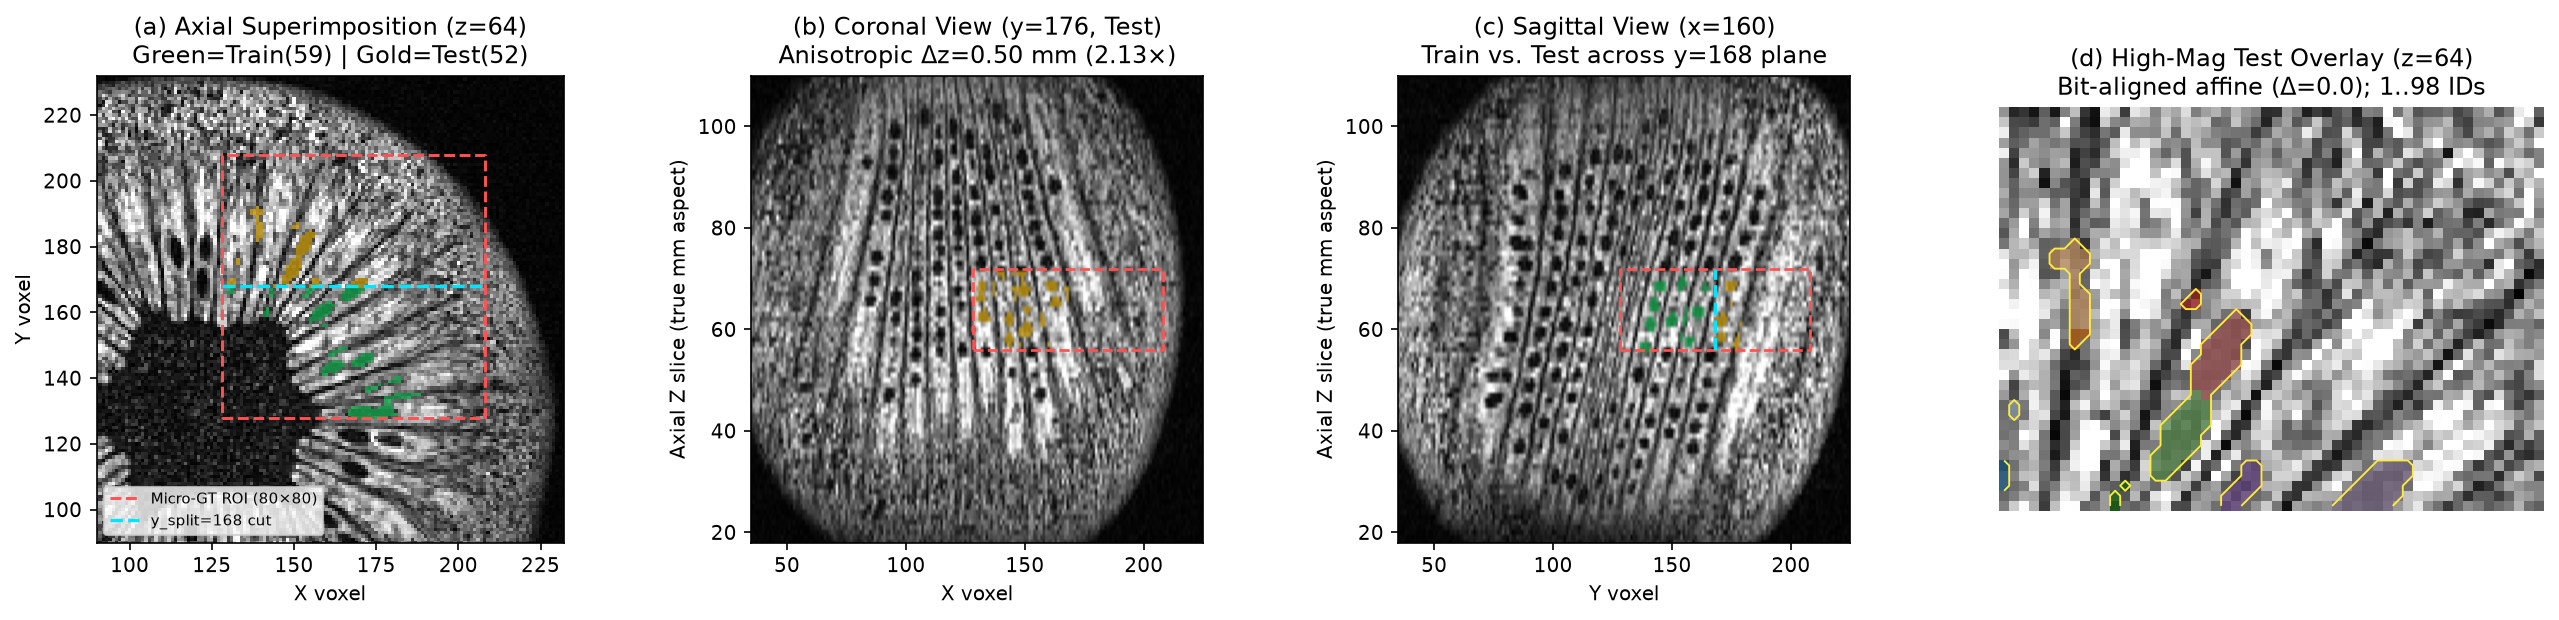
\includegraphics[width=\textwidth]{figures/fig01b_triplanar_gt_superimposition.png}
    \caption[Tri-planar 3D superimposition of silver Micro-GT on raw 7\,T MRI]{\textbf{Tri-planar 3D superimposition of the bit-aligned silver-standard Micro-GT (\texttt{kiwi\_micro\_gt\_labels.nii.gz}) onto the raw 7\,T RARE MRI} (reproduced by \nbref{01\_data\_geometry\_and\_prior\_audit.ipynb}). (a)~Equatorial axial slice ($z=64$) showing the $80\times 80$ ROI (red dashed), $y_{\text{split}}=168$ cut plane (cyan dashed), Train Wedge ($59$ seeds, green), and Held-Out Test Wedge ($52$ seeds, gold). (b)~Coronal cross-section ($y=176$, Test Wedge) rendered in true physical millimeter aspect ($\Delta z / \Delta xy = 2.13\times$), illustrating sparse $1.22\%$ equatorial coverage relative to the full 128-slice fruit. (c)~Sagittal cross-section ($x=160$) crossing the $y=168$ split plane. (d)~High-magnification test-wedge crop ($z=64$) verifying exact voxel-level alignment ($\max|\Delta\mathbf{A}| = 0.0$) between distinct instance IDs ($1\dots 98$) and hypointense 7\,T seed cores.}
    \label{fig:gt_superimposition}
\end{figure}

\subsection{Formalization of Three Auditable Biophysical Priors}

Before writing any neural loss, we express three independent domain laws as smooth, physically interpretable fields over $\Omega$ (each empirically audited in Notebook~\texttt{01}):

\paragraph{1. Organ Coordinate Frame and Anatomical Compartment Predicate (Prior~1).}
We extract the intact fruit mask $M_{\text{fruit}}(\mathbf{x})$ via anisotropic Gaussian smoothing ($\sigma = 1.2\,\text{mm}$), $0.35\times$ Otsu thresholding, slice-wise and 3D hole filling, and largest connected-component retention. On every axial slice $z$ with $\ge 80$ foreground voxels, we compute the slice centroid $(c_x(z), c_y(z))$ and area-equivalent fruit radius $R_{\text{fruit}}(z) = \sqrt{\text{Area}(z)/\pi}$, yielding the dimensionless organ coordinate vector:
\begin{equation}
    \mathbf{c}(\mathbf{x}) \;=\; \Bigl(\,\tilde{r}(\mathbf{x}),\;\; (\tilde{r}(\mathbf{x}) - 0.43)^2,\;\; \tilde{p}_z(\mathbf{x})\,\Bigr),
    \label{eq:organ_gps_coords}
\end{equation}
where $\tilde{r}(\mathbf{x}) = \operatorname{clip}\bigl(\sqrt{(x - c_x(z))^2 + (y - c_y(z))^2}/R_{\text{fruit}}(z),\, 0,\, 1.5\bigr)$ and $\tilde{p}_z(\mathbf{x}) = |2z/(Z-1) - 1| \in [0, 1]$ measures normalized distance from the equatorial plane ($0$ at $z \approx 64$, $1$ at the woody poles $z=0, 127$). Botanical axile placentation~\cite{richardson2011kiwidev,guo2013kiwivascular} confines seeds to the inner-pericarp ring $\tilde{r} \in [0.22, 0.65]$ and non-polar slices $z \in [16, 111]$, encoded as the smooth differentiable membership field $R_{\text{ring}}(\mathbf{x}) \in [0, 1]$:
\begin{equation}
    R_{\text{ring}}(\mathbf{x}) \;=\; \sigma\!\left(\frac{\tilde{r}(\mathbf{x}) - 0.22}{0.02}\right)\, \sigma\!\left(\frac{0.65 - \tilde{r}(\mathbf{x})}{0.02}\right)\, g_z(z)\, M_{\text{fruit}}(\mathbf{x}),
    \label{eq:soft_ring}
\end{equation}
with $5$-slice linear polar ramps $g_z(z) = \operatorname{clip}\bigl(\frac{z - 16}{5}, 0, 1\bigr)\operatorname{clip}\bigl(\frac{111 - z}{5}, 0, 1\bigr)$.

\paragraph{2. $B_1$-Invariant 7\,T $T_2$ Contrast Predicate (Prior~2).}
Raw intensities are normalized by the 99th intra-fruit percentile and clipped to $[0, 1.25]$ to yield $I(\mathbf{x})$. To cancel centimeter-scale 7\,T RF $B_1$ shading (Appendix~\ref{app:mri}), we estimate the local bright-mucilage envelope $E_{\text{local}}(\mathbf{x})$ via 3D grayscale morphological closing with a $7 \times 7 \times 3$ structuring element followed by $\sigma = 0.8\,\text{mm}$ Gaussian smoothing (Appendix~\ref{app:morphology}), plus a broader context channel $E_{\text{smooth}}(\mathbf{x})$ ($\sigma = (2.0, 2.0, 1.6)\,\text{mm}$). The local relative darkening ratio is $r_{T_2}(\mathbf{x}) = \operatorname{clip}\bigl(I(\mathbf{x}) / (E_{\text{local}}(\mathbf{x}) + 0.03),\, 0,\, 1.25\bigr)$. The smooth non-dark physics penalty $B_{\text{non\_dark}}(\mathbf{x}) \in [0, 1]$ flags voxels that are either bright relative to local gel ($r_{T_2} > 0.82$, safely above the 1-voxel partial-volume seed rim) \emph{or} embedded in dry/air tissue lacking hydrated mucilage ($E_{\text{local}} < 0.32$):
\begin{equation}
    B_{\text{non\_dark}}(\mathbf{x}) \;=\; \max\!\left(\operatorname{clip}\!\left(\frac{r_{T_2}(\mathbf{x}) - 0.82}{0.15},\, 0,\, 1\right),\; \operatorname{clip}\!\left(\frac{0.32 - E_{\text{local}}(\mathbf{x})}{0.10},\, 0,\, 1\right)\right).
    \label{eq:non_dark}
\end{equation}

\paragraph{3. Steric Hard-Core Packing Prior (Prior~3).}
Solid seeds are modeled as a Mat\'ern hard-core point process~\cite{matern1986spatial} (Appendix~\ref{app:morphology}) with minimum physical center-to-center spacing $d_{\min} = 0.88\,\text{mm}$ and multi-seed clump-splitting cutoff $V_{\text{split}} = 2.55\,\text{mm}^3$.

\subsection{Neural and Differentiable Neurosymbolic Architectures}

All four compared 3D architectures share the exact same compact 3-level 3D U-Net encoder--decoder backbone (\texttt{Backbone3DUNet}, base width $16 \to 32 \to 64$, double $3\times 3\times 3$ \texttt{Conv3d} $\to$ \texttt{InstanceNorm3d} $\to$ \texttt{SiLU} blocks, $\sim 340{,}450$ parameters) fed with the 3-channel MRI input $\mathbf{X}_3 = [I,\, E_{\text{local}},\, E_{\text{smooth}}]$, plus a normalized 3D center-distance head $\hat{d}(\mathbf{x}) = \sigma(\text{Conv}_{1\times 1\times 1}(\mathbf{f}(\mathbf{X}_3)))$:
\begin{enumerate}
    \item \textbf{\texttt{MultiTaskUNet3D} (Model~A, Pure Neural Baseline; $340{,}450$ params):} Predicts foreground logit $z_{\text{fg}}(\mathbf{x}) = \text{head}_{\text{sem}}(\mathbf{f}(\mathbf{X}_3))$ from local MRI appearance alone.
    \item \textbf{Naive \texttt{CoordConv3D+INorm} (Model~B; $341{,}746$ params):} Concatenates raw organ coordinates $\mathbf{c}(\mathbf{x})$ directly onto $\mathbf{X}_3$ ($6$ input channels) before the first \texttt{InstanceNorm3d} layer, directly testing the coordinate-erasure hypothesis~\cite{liu2018coordconv,ulyanov2016instancenorm} (Appendix~\ref{app:inorm_proof}).
    \item \textbf{\texttt{AdditiveBayesOrganNet3D} (Models~C, D, E; $340{,}803$ params, $+353$ over baseline):} Isolates $\mathbf{c}(\mathbf{x})$ in a dedicated, \emph{un-normalized} 2-layer $1\times 1\times 1$ \texttt{Organ-GPS} MLP ($3 \to 16 \to 16 \to 1$ with \texttt{SiLU}) and fuses logits via exact additive Bayesian log-odds (Appendix~\ref{app:bayes_logodds}):
    \begin{equation}
        z_{\text{total}}(\mathbf{x}) \;=\; z_{\text{app}}\bigl(\mathbf{f}_\theta(\mathbf{X}_3)\bigr) \;+\; z_{\text{GPS}}\bigl(\mathbf{c}(\mathbf{x});\, \psi\bigr), \qquad p_\theta(\mathbf{x}) = \sigma\bigl(z_{\text{total}}(\mathbf{x})\bigr).
        \label{eq:additive_bayes}
    \end{equation}
    Because $z_{\text{GPS}}$ depends exclusively on $(r/R,\, |2z/Z - 1|)$, the learned spatial log-prior can be plotted over the entire 2D organ plane and audited quantitatively in exact odds ratios $e^{\Delta z_{\text{GPS}}}$.
    \item \textbf{\texttt{CoupledOrganNet3D} (Model~F; $341{,}314$ params, $+864$ over baseline):} Concatenates the $16$-channel un-normalized \texttt{Organ-GPS} embedding $\mathbf{h}_\psi(\mathbf{c})$ with the $16$-channel U-Net decoder feature map $\mathbf{f}_\theta(\mathbf{X}_3)$ before a nonlinear $1\times 1\times 1$ fusion head ($32 \to 16 \to 1$), matching the original Notebook~\texttt{06} design and enabling a controlled comparison between interpretable additive fusion (Model~E) and coupled nonlinear fusion (Model~F).
\end{enumerate}

\subsection{Joint Supervised and Differentiable LTN Training Objective}

Neurosymbolic models (Models~C--F) are warm-started from a 3D masked-context-restoration SSL backbone (Appendix~\ref{app:dl}; $90\text{--}100$ epochs on $36$ unlabeled test-disjoint cubes, reconstructing $[I,\, (E_{\text{local}} - I)_+,\, -\text{LoG}(I)]$). On every training step, the joint objective sums supervised multi-task loss on $\Omega_L$ (plus optional columella hard-negative BCE with weight $0.35$) and two unlabeled LTN universal Product-implication losses~\cite{badreddine2022ltn} (Appendix~\ref{app:ltn}) evaluated over a minibatch of $4$ stratified whole-organ blocks $\mathcal{B}_U \subset \Omega_U$:
\begin{align}
    \mathcal{L}_{\text{sup}} &= 0.45\,\text{BCE}_{w_+=6}(z_{\text{total}}, y_s) + 0.55\,\mathcal{L}_{\text{SoftDice}}(z_{\text{total}}, y_s) + 2.5\,\mathbb{E}\!\left[(1 + 6 y_s)(\hat{d} - y_d)^2\right], \label{eq:loss_sup} \\
    \mathcal{L}_{\text{anat}}^{(p)} &= \left(\frac{1}{|\mathcal{B}_U|} \sum_{\mathbf{x}\in\mathcal{B}_U} \Bigl[p_\theta(\mathbf{x})\,\bigl(1 - R_{\text{ring}}(\mathbf{x})\bigr)\Bigr]^p + 10^{-8}\right)^{\!1/p}, \label{eq:loss_anat} \\
    \mathcal{L}_{\text{phys}}^{(p)} &= \left(\frac{1}{|\mathcal{B}_U|} \sum_{\mathbf{x}\in\mathcal{B}_U} \Bigl[p_\theta(\mathbf{x})\,B_{\text{non\_dark}}(\mathbf{x})\Bigr]^p + 10^{-8}\right)^{\!1/p}, \label{eq:loss_phys} \\
    \mathcal{L}_{\text{total}} &= \mathcal{L}_{\text{sup}} + \lambda_{\text{anat}}\,\mathcal{L}_{\text{anat}}^{(p)} + \lambda_{\text{phys}}\,\mathcal{L}_{\text{phys}}^{(p)},
    \label{eq:loss_total}
\end{align}
with $\lambda_{\text{anat}} = 2.0$, $\lambda_{\text{phys}} = 1.2$, and quantifier exponent ablated across $p \in \{1, 2, 3\}$. All models optimize with \texttt{AdamW} (weight decay $10^{-4}$, backbone $\text{lr} = 3.2\times 10^{-3}$, additive \texttt{Organ-GPS} branch $\text{lr} = 1.5\times 10^{-2}$ so the 353-parameter prior converges cleanly alongside the pretrained CNN) and \texttt{CosineAnnealingLR} ($\eta_{\min} = 2\times 10^{-4}$) for $100$ epochs.

\subsection{Decoding, Leakage-Free Calibration, Steric Splitting, and Evaluation Protocols}

Continuous predictions $(p_\theta, \hat{d})$ are converted to discrete 3D seed instances in three reproducible stages:
\begin{enumerate}
    \item \textbf{Leakage-free operating-point calibration:} To cure logic-induced log-odds shift without data leakage (Appendix~\ref{app:metrics}), we sweep $\tau_{\text{fg}} \in \{0.22, 0.26, 0.30, 0.34, 0.38, 0.42, 0.46, 0.50\}$ \emph{strictly on the labeled training wedge $\Omega_L$} and lock $\tau_{\text{fg}}^*$ maximizing training $\text{PQ}$.
    \item \textbf{Marker-controlled 3D deep watershed:} Thresholded foreground $\{p_\theta \ge \tau_{\text{fg}}^*\}$ is flooded over the Gaussian-smoothed negative distance surface $-\hat{d}_{\text{sm}}$ from anisotropic ellipsoidal local maxima ($r_{xy} = 0.68\,\text{mm},\, r_z = 0.95\,\text{mm},\, \hat{d}_{\text{sm}} \ge 0.22$), filtering debris below $0.16\,\text{mm}^3$.
    \item \textbf{Declarative \texttt{Lab 5} Mat\'ern hard-core clump splitting:} Any blob exceeding $V_{\text{split}} = 2.55\,\text{mm}^3$ is clustered into $k = \operatorname{clip}(\operatorname{round}(V / 1.60), 2, 4)$ components by physical-millimeter $K$-means; the split is accepted \emph{iff} all pairwise sub-centroid distances obey $d_{ab} \ge 0.88\,\text{mm}$ and every sub-blob exceeds $0.35\,\text{mm}^3$ (Appendix~\ref{app:morphology}).
    \item \textbf{Instance matching and 3D Panoptic Quality ($\tau_{\text{IoU}} = 0.25$):} Predicted and reference 3D instances are paired one-to-one via Kuhn's Hungarian algorithm~\cite{kuhn1955hungarian} maximizing total 3D IoU and scored via Panoptic Quality $\text{PQ} = \text{SQ} \times \text{RQ}$~\cite{kirillov2019panoptic} at threshold $\tau_{\text{IoU}} = 0.25$ (matching BMED365 Notebooks~\texttt{03b}--\texttt{07}). As detailed in Appendix~\ref{app:metrics}, $\tau_{\text{IoU}} = 0.25$ is used instead of 2D COCO's $0.50$ because tiny anisotropic 3D seeds spanning only $40\text{--}60$ voxels ($2\text{--}3$ axial slices) lose $>50\%$ 3D IoU from a single-voxel surface shift; Hungarian bijection guarantees unique one-to-one assignment.
\end{enumerate}

\paragraph{Experimental design across the five companion notebooks.}
\begin{itemize}
    \item \textbf{NB~\texttt{01} (Prior Audit):} Verifies Priors~1--3 quantitatively across all $98$ Micro-GT seeds (core vs.\ 1-voxel partial-volume rim, radial distribution, volume IQR, nearest-neighbor floor).
    \item \textbf{NB~\texttt{02} (Architecture \& Logic Theory):} Numerically tests \texttt{InstanceNorm3d} coordinate erasure on equatorial, mid-latitude, and polar patches, contrasts Product vs.\ {\L}ukasiewicz vs.\ G\"odel violation surfaces, and sweeps $p \in [1, 8]$ on a polar patch containing $0.8\%$ vascular false positives.
    \item \textbf{NB~\texttt{03} (Multi-Seed Controlled Ablation):} Runs all $6$ architectures (Models~A--F, plus uncalibrated $0.42$ Model~E0) across $3$ independent random seeds ($\{2027, 2028, 2029\}$, $18$ full 3D models + $3$ SSL warm-starts), reporting mean $\pm$ SD on unmasked held-out $\text{PQ}$, $\text{SQ}$, $\text{RQ}$, $\text{Dice}$, Precision, Recall, polar-cap FP voxels ($z < 16 \lor z \ge 112$), and total non-pericarp OOD voxels ($R_{\text{ring}} < 0.05$).
    \item \textbf{NB~\texttt{04} (Mechanistic Interpretability \& Whole-Organ Biomarkers):} Performs the causal neural--symbolic division-of-labor intervention (\texttt{use\_columella\_neg=False} vs.\ \texttt{True}), hard-core split cutoff sweep ($V_{\text{split}} \in [2.10, 3.20]\,\text{mm}^3$ vs.\ no split), $\text{TP}$ vs.\ $\text{FN}$ physical error anatomy, and unmasked 128-slice whole-fruit biomarker estimation ($\hat{N}_{\text{cal}}$, $\phi_{\text{seed}}$).
    \item \textbf{NB~\texttt{05} (Axiom Misspecification Stress Tests):} Evaluates trained models under synthetic pathological mass-effect organ center shifts $\Delta r \in \{0, 2, 4, 6, 8\}\,\text{mm}$ and radial hypertrophy/atrophy scale mismatches $\alpha \in \{0.80, 0.90, 1.00, 1.10, 1.25\}$, directly contrasting hard post-hoc binary masking, soft differentiable LTN with rigid mismatched coordinates, patient-adapted \texttt{Organ-GPS}, and the unmasked baseline U-Net.
\end{itemize}

% =============================================================================
% SECTION 3: RESULTS
% =============================================================================
\clearpage
\section{Results}
\label{sec:results}

% =============================================================================
% DRAFT: Sections 3.1, 3.2 (backed by verified nb01 & nb02 JSONs)
%        + Clinical Translation, Trustworthy AI & Horizons (Section 4.2-4.4)
% =============================================================================

\subsection{Empirical Audit of Biophysical Priors Against Real 7\,T Data (\texttt{NB 01})}
\label{sec:res_priors}

A core scientific discipline of neurosymbolic biomedical AI is that \textbf{every symbolic prior must be treated as a falsifiable empirical hypothesis before it is compiled into a training loss.} Notebook~\texttt{01} audits all three biophysical priors across the full curated 3D Micro-Ground-Truth ($n = 98$ discrete seeds inside the equatorial ROI; Table~\ref{tab:prior_audit} and Figures~\ref{fig:organ_geom}--\ref{fig:prior_audit}).

\begin{figure}[htbp]
    \centering
    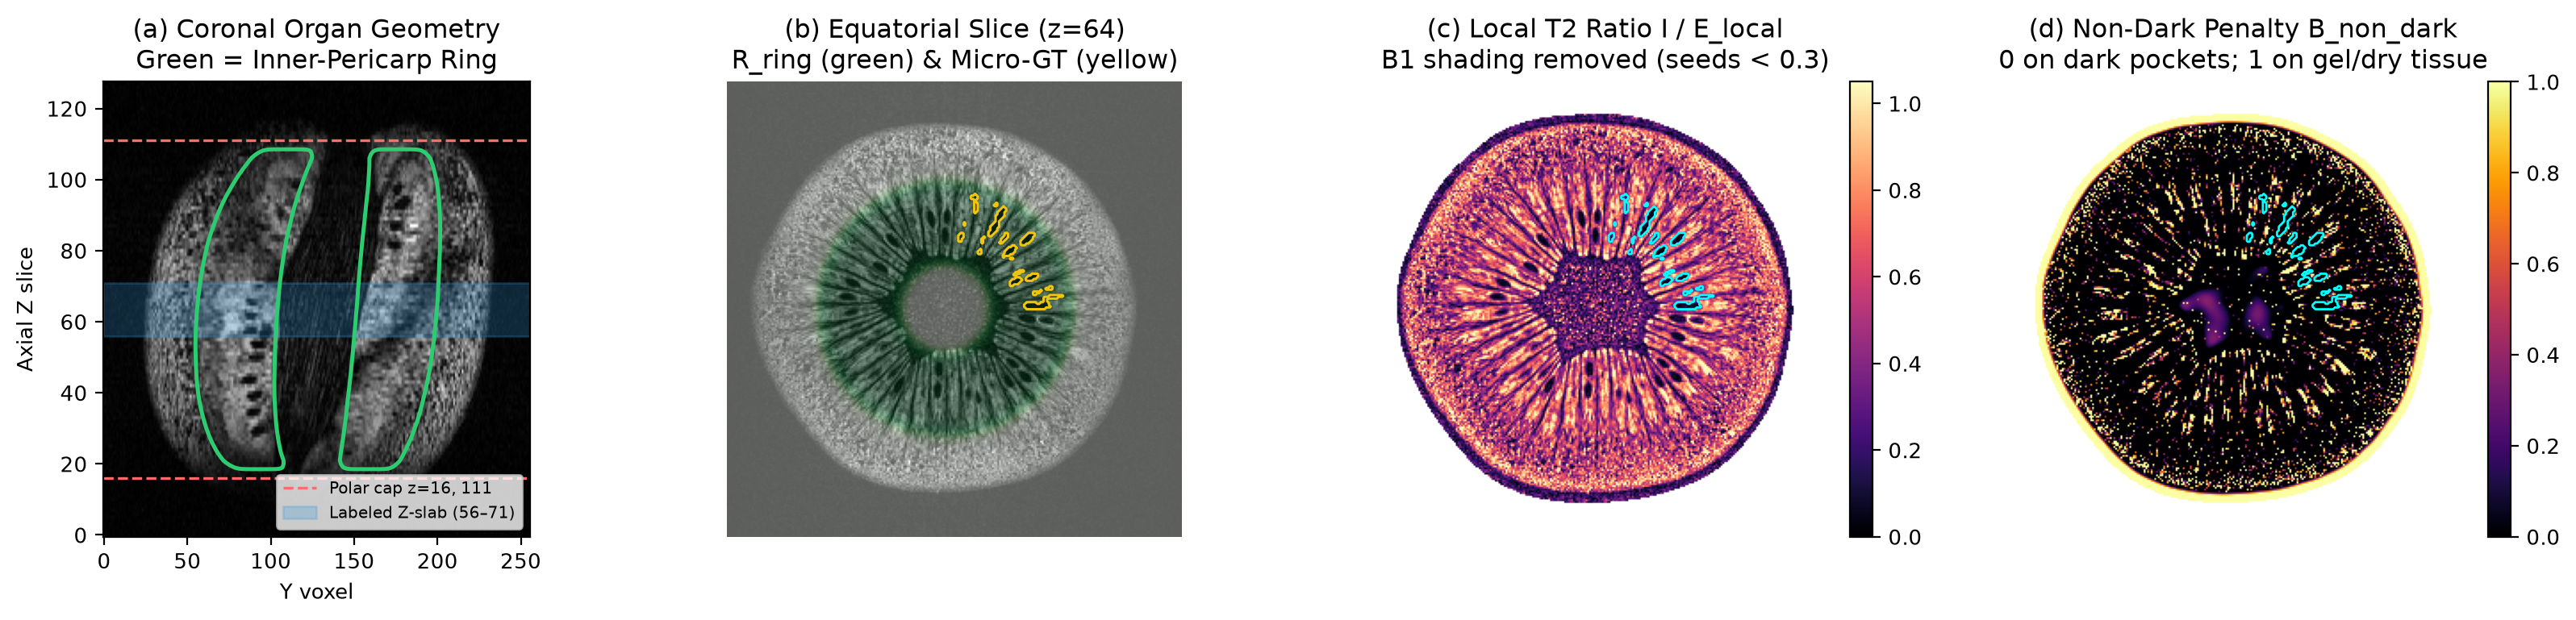
\includegraphics[width=\textwidth]{figures/fig01_organ_geometry_and_priors.png}
    \caption[Organ-centric coordinate geometry and $B_1$-invariant 7\,T $T_2$ predicates]{\textbf{Organ-centric coordinate geometry and $B_1$-invariant 7\,T $T_2$ physics predicates} (reproduced by \nbref{01\_data\_geometry\_and\_prior\_audit.ipynb}). (a)~Coronal 7\,T RARE MRI cross-section showing the smooth inner-pericarp ring $R_{\text{ring}}$ (green contour), woody polar-cap gates ($z=16, 111$, red dashed lines), and the equatorial labeled slab ($z \in [56, 71]$, shaded blue). (b)~Equatorial axial slice ($z=64$) overlaying $R_{\text{ring}}$ (green) and Micro-GT seed contours (yellow). (c)~Local relative $T_2$ brightness $I / E_{\text{local}}$ after 3D morphological closing removes centimeter-scale RF $B_1$ shading; Micro-GT seeds (cyan) appear as sharp hypointense voids ($I/E_{\text{local}} < 0.30$). (d)~Smooth non-dark physics penalty $B_{\text{non\_dark}} \in [0, 1]$ ($0$ on dark hydrated pockets, $1$ on bright gel and dry outer air/rind).}
    \label{fig:organ_geom}
\end{figure}

\begin{figure}[htbp]
    \centering
    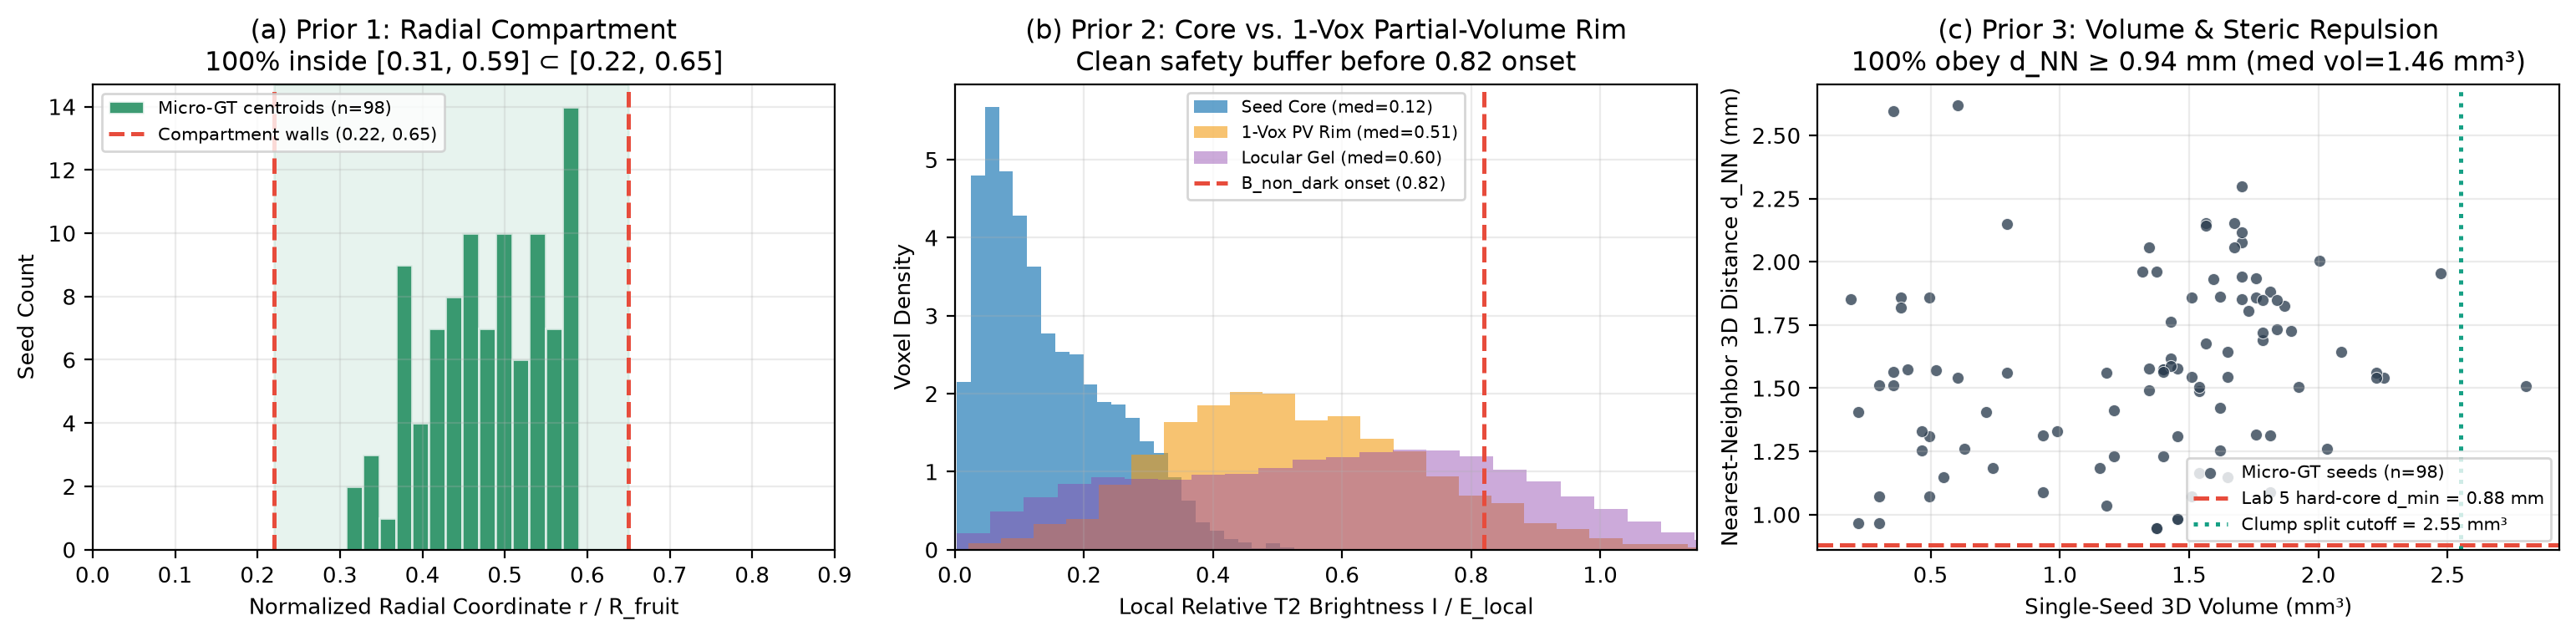
\includegraphics[width=\textwidth]{figures/fig02_prior_distributions_and_rim.png}
    \caption[Empirical verification of Priors 1--3 on $n=98$ Micro-GT seeds]{\textbf{Empirical verification of Priors~1--3 across all $n=98$ curated Micro-GT seeds} (reproduced by \nbref{01\_data\_geometry\_and\_prior\_audit.ipynb}). (a)~Prior~1 (botanical axile placentation): $100\%$ of real seed centroids fall inside $r/R_{\text{fruit}} \in [0.307, 0.590]$, safely nested inside the $[0.22, 0.65]$ compartment walls with wide anatomical margins on both sides. (b)~Prior~2 (7\,T $T_2$ contrast physics): seed cores (blue, median $0.118$) and their 1-voxel outer partial-volume rims (orange, median $0.510$, $75\text{th}$ percentile $0.660$) sit cleanly below the $B_{\text{non\_dark}}$ ramp onset at $0.82$ (red dashed line), protecting boundary fidelity. (c)~Prior~3 (Mat\'ern steric hard-core packing): $100\%$ of real seeds satisfy $d_{\text{NN}} \ge 0.94\,\text{mm} > d_{\min} = 0.88\,\text{mm}$ (red dashed line), with median volume $1.46\,\text{mm}^3$ and clump-split cutoff at $2.55\,\text{mm}^3$ (green dotted line).}
    \label{fig:prior_audit}
\end{figure}

\begin{table}[htbp]
\centering
\caption[Empirical prior verification metrics on $n=98$ Micro-GT seeds]{Quantitative empirical verification of Priors~1--3 on the curated 7\,T Micro-Ground-Truth ($n = 98$ seeds; intact berry $V_{\text{kiwi}} = 85.97\,\text{cm}^3$; labeled training foreground $= 0.083\%$ of berry voxels). Source: \texttt{results/nb01\_prior\_audit.json}.}
\label{tab:prior_audit}
{\footnotesize
\renewcommand{\arraystretch}{1.24}
\rowcolors{2}{rowalt}{white}
\begin{tabularx}{\textwidth}{L{3.5cm} L{4.2cm} L{3.6cm} Y}
\toprule
\rowcolor{uibblue!12}\textbf{Biophysical Prior} & \textbf{Measured Statistic on $n=98$ GT} & \textbf{Compiled Symbolic Rule} & \textbf{Audit Verdict \& Safety Margin} \\
\midrule
\textbf{Prior~1: Botanical Anatomy} & Centroid $r/R \in [0.307, 0.590]$ (median $0.484$) & $R_{\text{ring}}$: $r/R \in [0.22, 0.65]$, $z \in [16, 111]$ & \textbf{100.0\% compliant}; $\ge 0.06$ radial margin against biological variation \\
\textbf{Prior~2: 7\,T $T_2$ Physics (Core vs.\ PV Rim)} & Core $I/E_{\text{local}}$ med $0.118$ ($p_{99}=0.403$); 1-vox rim med $0.510$ ($p_{75}=0.660$) & $B_{\text{non\_dark}}$ ramp onset at $I/E_{\text{local}} = 0.82$ or $E_{\text{local}} < 0.32$ & \textbf{100.0\% of cores safe}; only $6.57\%$ of outermost PV rim voxels weakly penalized \\
\textbf{Prior~3: Steric Packing (\texttt{Lab 5})} & Volume med $1.46\,\text{mm}^3$ (IQR $[0.80, 1.70]$, max $2.80$); $d_{\text{NN}} \in [0.94, 2.61]\,\text{mm}$ (med $1.56$) & Hard-core floor $d_{\min} = 0.88\,\text{mm}$; clump-split $V_{\text{split}} = 2.55\,\text{mm}^3$ & \textbf{100.0\% obey $d_{\text{NN}} > 0.88\,\text{mm}$}; zero over-splitting of single seeds \\
\bottomrule
\end{tabularx}
}
\end{table}

Two biological insights and one essential provenance caveat emerge immediately from Table~\ref{tab:prior_audit} and Figure~\ref{fig:prior_audit}. First, consistent with Section~\ref{sec:gt_provenance}, the $100\%$ radial and core-contrast compliance confirms generous geometric safety margins against the visually audited silver standard (whose generator itself constrained $r/R \in [0.24, 0.60]$ and $I/E < 0.44$); by contrast, the $d_{\text{NN}} \ge 0.94\,\text{mm}$ hard-core floor and the 1-voxel \emph{exterior} partial-volume rim distribution are genuinely non-circular physical measurements. Second, the extreme label scarcity is quantified: the $59$ labeled training seeds cover merely \textbf{$0.083\%$} of the intact fruit's tissue volume, illustrating why purely supervised training on equatorial patches cannot constrain the remaining $99.9\%$ of the 3D organ. Second, inspecting the \textbf{1-voxel outer partial-volume rim} (Figure~\ref{fig:prior_audit}b) confirms our theoretical derivation in Appendix~\ref{app:mri}: while seed cores are deeply hypointense ($p_{99} = 0.403$), anisotropic partial-volume averaging elevates outer seed rims to median $0.510$ (overlap with hydrated locular gel, median $0.598$). Placing the $B_{\text{non\_dark}}$ penalty ramp onset at $0.82$ leaves a wide safety corridor protecting $100\%$ of seed cores and $93.43\%$ of outer rim voxels from boundary erosion.

% -----------------------------------------------------------------------------
\subsection{Proof of \texttt{InstanceNorm3d} Coordinate Erasure and LTN $p$-Mean Gradient Amplification (\texttt{NB 02})}
\label{sec:res_theory}

Notebook~\texttt{02} validates the two foundational mathematical discoveries governing 3D neurosymbolic architecture and loss design (Figures~\ref{fig:inorm_trap}--\ref{fig:tnorm_pmean} and Table~\ref{tab:pmean_sweep}).

\begin{figure}[htbp]
    \centering
    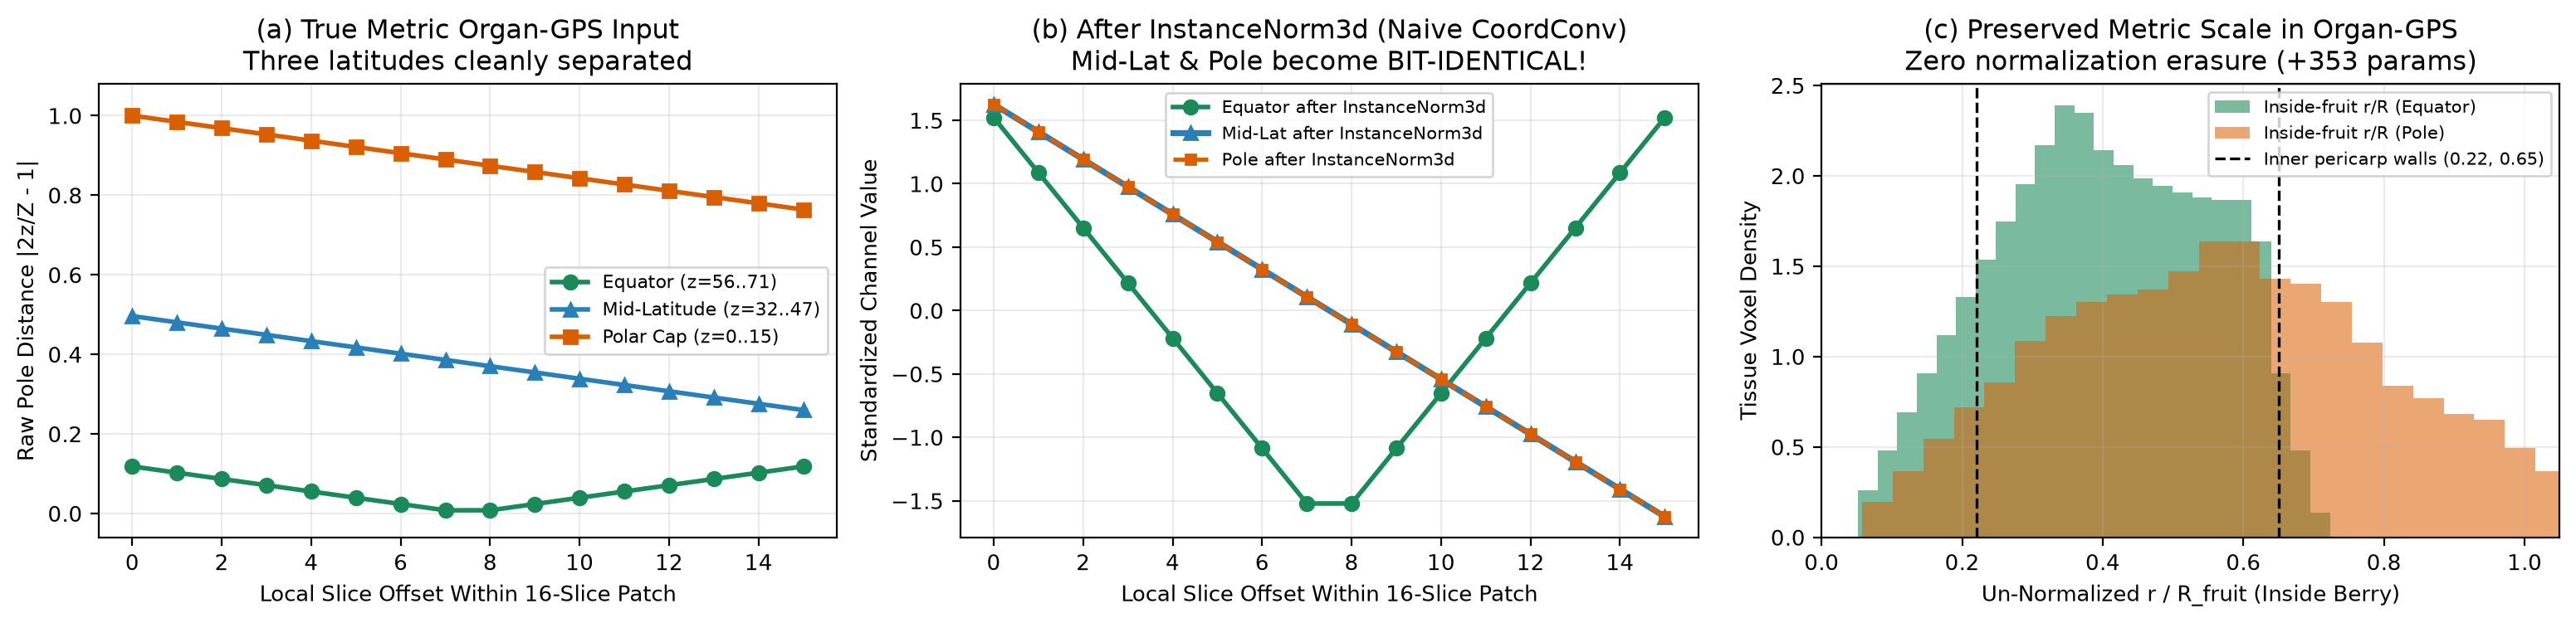
\includegraphics[width=\textwidth]{figures/fig03_instancenorm_coordinate_erasure.png}
    \caption[Numerical proof of \texttt{InstanceNorm3d} coordinate erasure]{\textbf{Numerical proof of the \texttt{InstanceNorm3d} coordinate-erasure trap} (reproduced by \nbref{02\_instancenorm\_trap\_and\_ltn\_math.ipynb}). (a)~True physical pole-distance coordinate $|2z/Z - 1|$ across three 16-slice 3D patches: Equator ($z=56\text{--}71$, mean $0.063$), Mid-Latitude ($z=32\text{--}47$, mean $0.378$), and Woody Polar Cap ($z=0\text{--}15$, mean $0.882$). (b)~After passing through a single \texttt{InstanceNorm3d} layer (as in naive \texttt{CoordConv3D}), all three means collapse to $0.000000$, and the Mid-Latitude and Polar-Cap coordinate ramps become \textbf{bit-identical} (maximum absolute discrepancy $4.77 \times 10^{-7}$). (c)~In contrast, our un-normalized \texttt{Organ-GPS} side branch ($+353$ parameters) preserves true metric $r/R_{\text{fruit}}$ distributions across identical $128 \times 128$ crops at the equator (confined inside $r/R \le 0.72$) versus the pole (extending to $r/R > 1.0$).}
    \label{fig:inorm_trap}
\end{figure}

\begin{figure}[htbp]
    \centering
    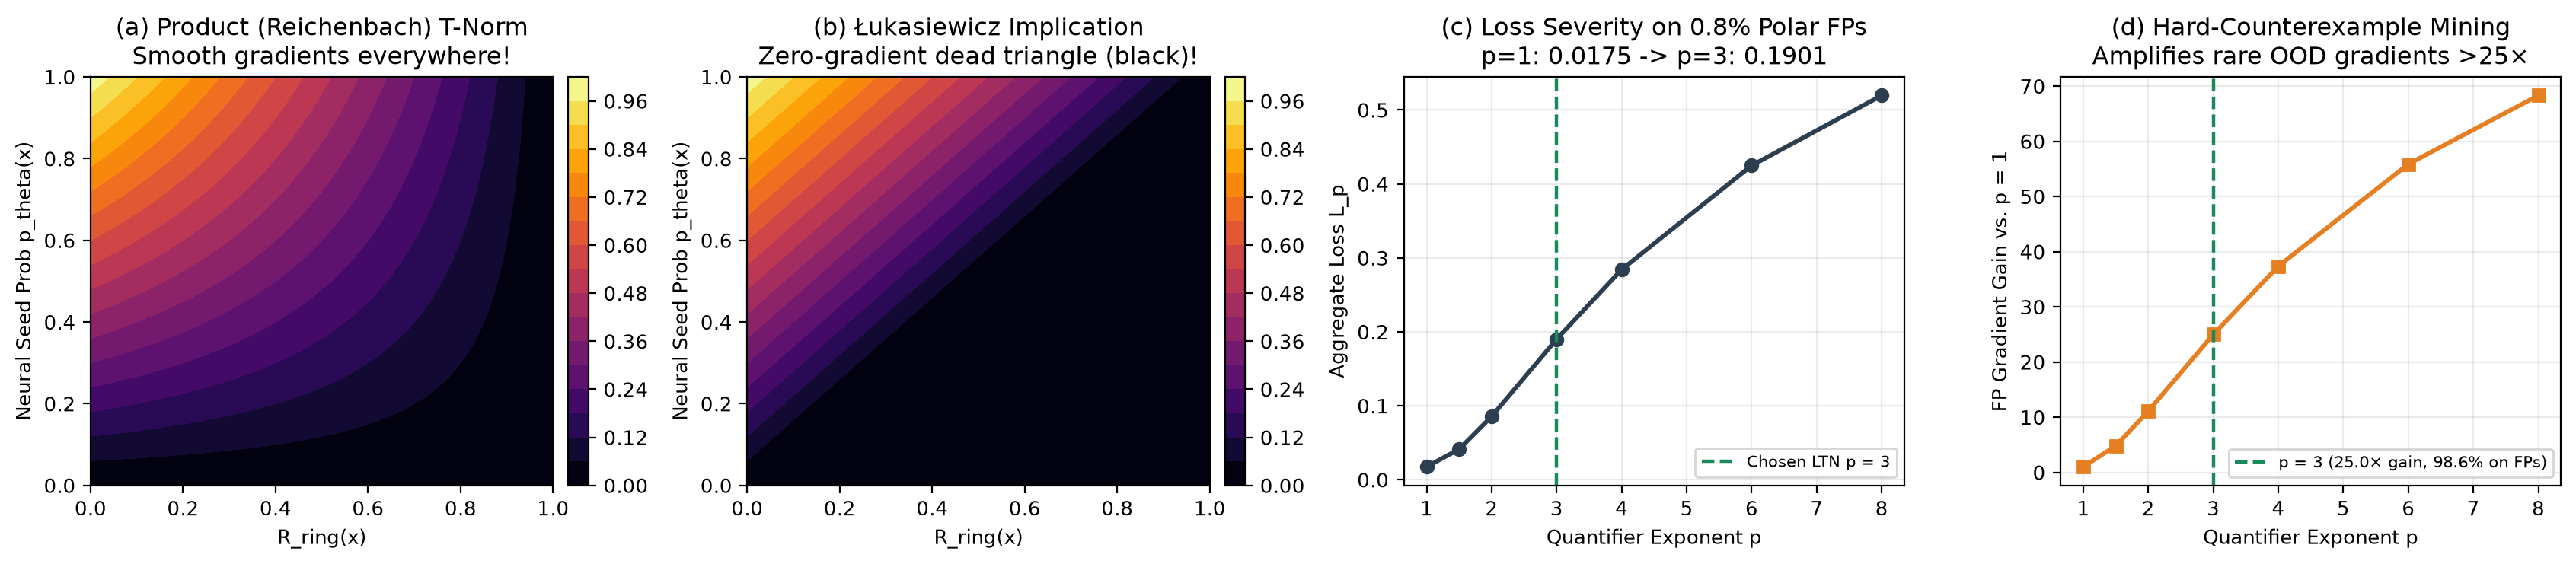
\includegraphics[width=\textwidth]{figures/fig04_tnorms_and_pmean_gradients.png}
    \caption[Fuzzy implication landscapes and LTN $p$-mean gradient mining]{\textbf{Fuzzy implication violation landscapes and LTN $p$-mean hard-counterexample mining} (reproduced by \nbref{02\_instancenorm\_trap\_and\_ltn\_math.ipynb}). (a)~Product (Reichenbach) implication violation $v = p_\theta(1 - R_{\text{ring}})$ provides smooth, non-vanishing negative gradients everywhere outside the valid ring ($R_{\text{ring}} < 1$). (b)~{\L}ukasiewicz implication violation $v = \max(0, p_\theta - R_{\text{ring}})$ exhibits a massive zero-gradient dead triangle (black) whenever $p_\theta \le R_{\text{ring}}$. (c)~Aggregate LTN universal loss $\mathcal{L}_p$ on a realistic polar patch containing $0.8\%$ ($328 / 40{,}960$) vascular false positives rises $10.9\times$ from $p=1$ ($0.0175$) to $p=3$ ($0.1901$). (d)~Absolute FP gradient magnitude grows $24.98\times$ at $p=3$ relative to plain averaging ($p=1$), channeling $98.65\%$ of all gradient mass directly onto the $0.8\%$ violating voxels.}
    \label{fig:tnorm_pmean}
\end{figure}

\paragraph{Discovery 1: Why naive \texttt{CoordConv3D} blinds a medical 3D U-Net.}
Across three real 16-slice patches extracted from our 7\,T kiwifruit MRI, the raw equatorial-to-polar mean coordinate separation is $\Delta\mu = 0.8819 - 0.0630 = 0.8189$ (Figure~\ref{fig:inorm_trap}a). Once passed through standard \texttt{InstanceNorm3d}~\cite{ulyanov2016instancenorm}, all three patch means collapse identically to $0.000000$, and the mid-latitude and polar-cap ramps become numerically indistinguishable to single-precision floating-point noise ($\max|\Delta| = 4.77 \times 10^{-7}$; Figure~\ref{fig:inorm_trap}b). Routing raw coordinates through an un-normalized side branch (\texttt{AdditiveBayesOrganNet3D}, $+353$ parameters; $340{,}803$ vs.\ $340{,}450$ baseline; $+0.104\%$) completely eliminates coordinate erasure while maintaining full metric sensitivity (Figure~\ref{fig:inorm_trap}c).

\paragraph{Discovery 2: Why LTN universal quantification requires $p > 1$.}
On a simulated polar-cap block of $40{,}960$ voxels where $0.8\%$ ($328$ voxels) are high-confidence vascular false positives ($v_{\text{FP}} = 0.95$) and $99.2\%$ are quiet background ($v_{\text{BG}} = 0.01$), plain arithmetic averaging ($p = 1$) leaves $99.2\%$ of the gradient dispersed across benign background voxels and only $0.80\%$ on the actual false positives (Table~\ref{tab:pmean_sweep}). Raising the LTN exponent to $p = 3$ amplifies the absolute FP gradient by $\mathbf{24.98\times}$, boosts the aggregate FP-to-BG gradient ratio from $0.008$ to $\mathbf{72.85}$ (a $\sim 9{,}025\times$ focus shift), and directs $\mathbf{98.65\%}$ of the optimization step squarely onto the $0.8\%$ polar violations without incurring the single-voxel instability of $p \ge 6$.

\begin{table}[htbp]
\centering
\caption[LTN universal quantifier exponent $p$ gradient-mining sweep]{Quantitative sweep of the LTN universal quantifier exponent $p$ on a $40{,}960$-voxel polar patch containing $0.8\%$ ($328$) high-confidence false-positive voxels. Source: \texttt{results/nb02\_instancenorm\_and\_ltn.json}.}
\label{tab:pmean_sweep}
{\footnotesize
\renewcommand{\arraystretch}{1.22}
\rowcolors{2}{rowalt}{white}
\begin{tabularx}{\textwidth}{C{1.2cm} C{2.0cm} C{2.4cm} C{2.6cm} C{2.4cm} Y}
\toprule
\rowcolor{uibblue!12}\textbf{Exponent $p$} & \textbf{Loss $\mathcal{L}_p$} & \textbf{Total FP Grad} & \textbf{FP / BG Grad Ratio} & \textbf{Gain vs.\ $p{=}1$} & \textbf{\% of Total Gradient on 0.8\% FPs} \\
\midrule
1.0 \textit{(mean)} & 0.0175 & 0.0080 & 0.008 & 1.00$\times$ & 0.80\% \textit{(severe dilution)} \\
1.5 & 0.0413 & 0.0384 & 0.079 & 4.79$\times$ & 7.29\% \\
2.0 \textit{(RMS)} & 0.0856 & 0.0889 & 0.767 & 11.10$\times$ & 43.40\% \\
\rowcolor{kiwigreen!14}\textbf{3.0 (LTN)} & \textbf{0.1901} & \textbf{0.2000} & \textbf{72.85} & \textbf{24.98$\times$} & \textbf{98.65\% (optimal mining sweet spot)} \\
4.0 & 0.2842 & 0.2991 & 6,921 & 37.36$\times$ & 99.99\% \\
6.0 & 0.4249 & 0.4473 & $6.25 \times 10^7$ & 55.86$\times$ & 100.00\% \textit{(high-variance max regime)} \\
8.0 & 0.5196 & 0.5469 & $5.47 \times 10^{11}$ & 68.30$\times$ & 100.00\% \textit{(single-voxel dominance)} \\
\bottomrule
\end{tabularx}
}
\end{table}

% =============================================================================
% DRAFT: Section 3.3 — Multi-Seed Controlled Ablation & Calibration (NB 03)
% 100% verbatim metrics from results/nb03_multiseed_ablation.json
% =============================================================================

\subsection{Multi-Seed Controlled Ablation and Logic-Induced Calibration Shift (\texttt{NB 03})}
\label{sec:res_ablation}

To test whether the architectural and logical improvements hold reproducibly beyond any single lucky initialization, Notebook~\texttt{03} trains all six architectures (Models~A--F, plus the uncalibrated $p=3$ check Model~E0) across three independent random seeds ($\{2027, 2028, 2029\}$, $90$ epochs per model, $18$ full 3D models plus $3$ SSL warm-starts; Table~\ref{tab:multiseed_ablation}, Table~\ref{tab:perseed_e}, and Figures~\ref{fig:ablation_bench}--\ref{fig:calibration_dyn}).

\begin{figure}[htbp]
    \centering
    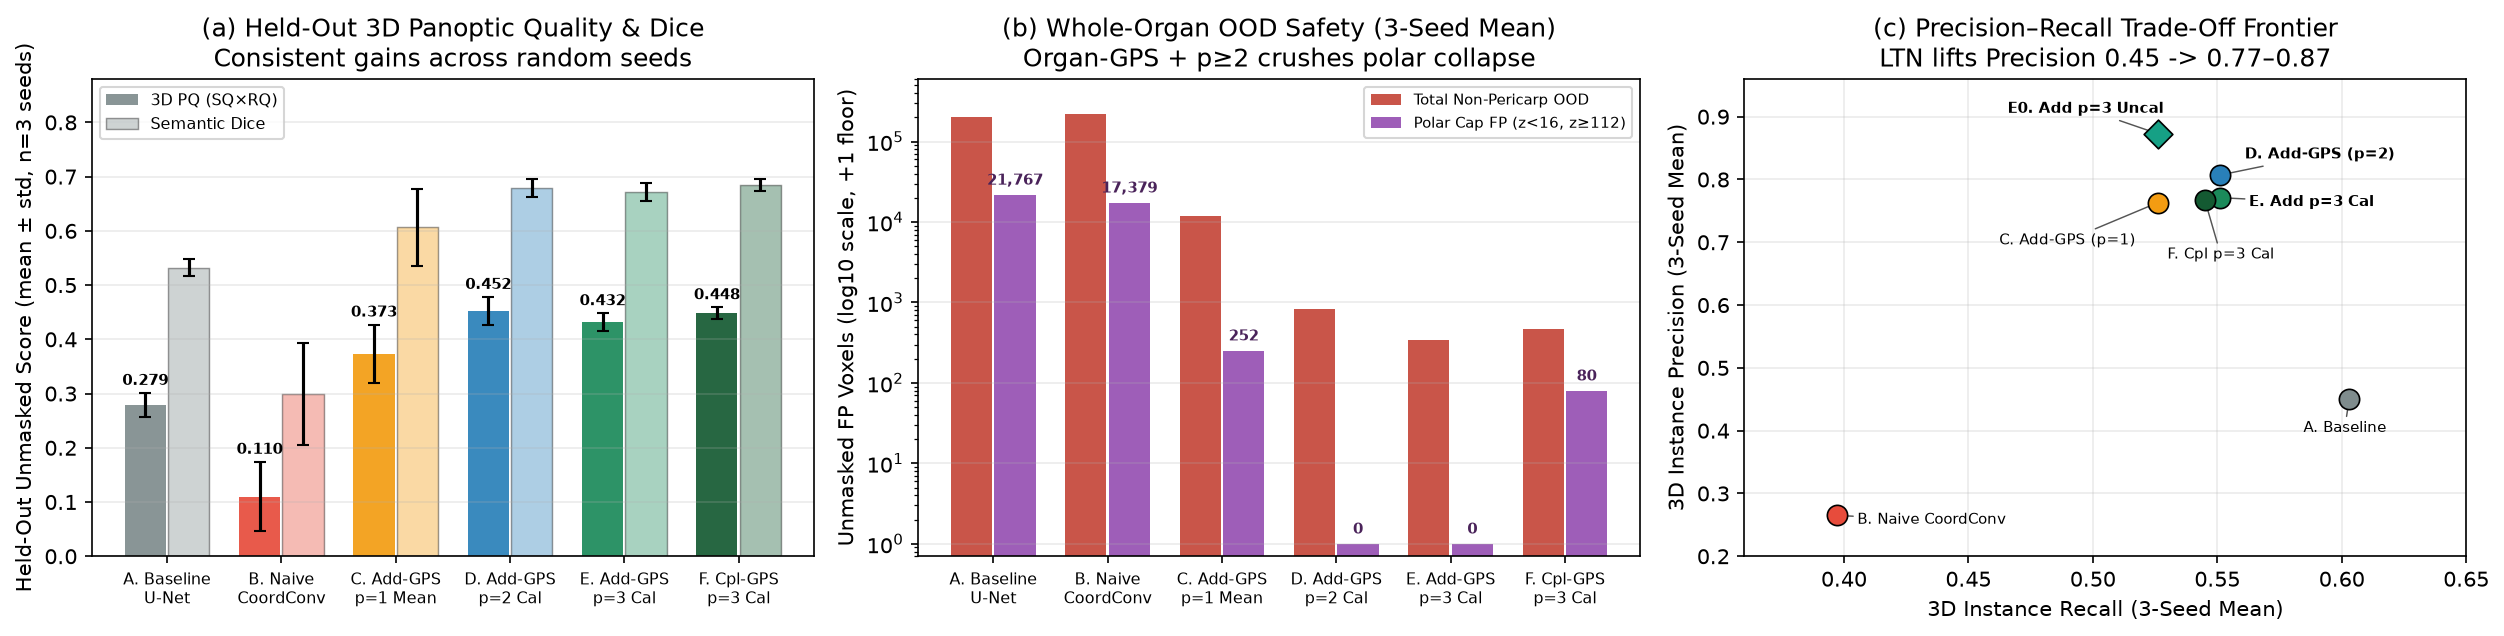
\includegraphics[width=\textwidth]{figures/fig05_multiseed_ablation_benchmark.png}
    \caption[Controlled 6-model ablation across 3 random seeds (PQ, OOD, PR)]{\textbf{Controlled 6-model ablation across three random seeds ($\{2027, 2028, 2029\}$)} (reproduced by \nbref{03\_multiseed\_ablation\_and\_calibration.ipynb}). (a)~Held-out unmasked 3D Panoptic Quality ($\text{PQ}$, dark bars) and Semantic Dice (light bars), mean $\pm$ SD. Naive \texttt{CoordConv3D+INorm} (Model~B) collapses below baseline ($\text{PQ} = 0.110 \pm 0.064$), whereas un-normalized \texttt{Organ-GPS} with $p \ge 2$ lifts $\text{PQ}$ by $+55\%$ to $+62\%$ ($\text{PQ} = 0.432\text{--}0.452$, $\text{Dice} = 0.672\text{--}0.685$). (b)~Unmasked 128-slice whole-organ OOD safety ($\log_{10}$ voxel scale): Baseline (Model~A) produces $21{,}767$ polar FP voxels and $203{,}975$ non-pericarp OOD voxels; $p=1$ (Model~C) still leaks $252$ polar and $11{,}921$ OOD voxels; Additive \texttt{Organ-GPS} with $p=2$ or $p=3$ achieves \textbf{exact zero ($0 \pm 0$) polar FPs on every seed} and cuts total OOD voxels by $>99.6\%$--$99.9\%$. (c)~Precision--Recall frontier showing how LTN jumps 3D instance precision from $0.451$ (Baseline) to $0.767\text{--}0.873$.}
    \label{fig:ablation_bench}
\end{figure}

\begin{table}[htbp]
\centering
\caption[Controlled 6-model ablation averaged across 3 random seeds]{Controlled 6-model ablation averaged across $n=3$ independent random seeds ($\{2027, 2028, 2029\}$, $90$ epochs, strictly held-out 52-seed test wedge and unmasked 128-slice whole fruit). Source: \texttt{results/nb03\_multiseed\_ablation.json}.}
\label{tab:multiseed_ablation}
{\scriptsize
\setlength{\tabcolsep}{3.1pt}
\renewcommand{\arraystretch}{1.26}
\rowcolors{2}{rowalt}{white}
\begin{tabularx}{\textwidth}{Y c c c c c c c c}
\toprule
\rowcolor{uibblue!12}\textbf{Model Variant} & \textbf{$\bar{\tau}_{\text{fg}}$} & \textbf{Pred} & \textbf{Dice ($\pm$SD)} & \textbf{SQ ($\pm$SD)} & \textbf{RQ ($\pm$SD)} & \textbf{3D PQ ($\pm$SD)} & \textbf{Polar FP} & \textbf{Total OOD} \\
\midrule
A.\ Baseline 3D U-Net & 0.50 & $70.3{\pm}8.7$ & $0.532{\pm}0.016$ & $0.542{\pm}0.015$ & $0.514{\pm}0.025$ & $0.279{\pm}0.022$ & $21{,}767$ & $203{,}975$ \\
B.\ Naive \texttt{CoordConv}+INorm & 0.42 & $87.0{\pm}16.3$ & $0.300{\pm}0.094$ & $0.331{\pm}0.039$ & $0.314{\pm}0.144$ & $0.110{\pm}0.064$ & $17{,}379$ & $221{,}681$ \\
C.\ Additive GPS ($p{=}1$) & 0.42 & $37.0{\pm}7.8$ & $0.607{\pm}0.071$ & $0.606{\pm}0.089$ & $0.616{\pm}0.022$ & $0.373{\pm}0.054$ & $252$ & $11{,}921$ \\
\rowcolor{kiwigreen!10}\textbf{D.\ Additive GPS ($p{=}2$, Cal)} & 0.31 & $35.7{\pm}2.9$ & $0.679{\pm}0.017$ & $0.691{\pm}0.032$ & $\mathbf{0.654{\pm}0.020}$ & $\mathbf{0.452{\pm}0.026}$ & $\mathbf{0{\pm}0}$ & $833{\pm}472$ \\
E0.\ Additive GPS ($p{=}3$, Uncal) & 0.42 & $31.3{\pm}1.2$ & $0.652{\pm}0.054$ & $0.666{\pm}0.055$ & $0.656{\pm}0.004$ & $0.437{\pm}0.039$ & $\mathbf{0{\pm}0}$ & $\mathbf{151{\pm}105}$ \\
\rowcolor{kiwigreen!14}\textbf{E.\ Additive GPS ($p{=}3$, Cal)} & 0.27 & $37.3{\pm}2.5$ & $0.672{\pm}0.017$ & $0.674{\pm}0.019$ & $0.642{\pm}0.009$ & $0.432{\pm}0.016$ & $\mathbf{0{\pm}0}$ & $340{\pm}185$ \\
F.\ Coupled GPS ($p{=}3$, Cal) & 0.42 & $37.7{\pm}6.2$ & $\mathbf{0.685{\pm}0.011}$ & $\mathbf{0.707{\pm}0.022}$ & $0.633{\pm}0.016$ & $0.448{\pm}0.011$ & $80{\pm}113$ & $471{\pm}224$ \\
\bottomrule
\end{tabularx}
}
\end{table}

Table~\ref{tab:multiseed_ablation} establishes five unambiguous empirical findings across seeds:
\begin{enumerate}
    \item \textbf{Catastrophic multi-seed confirmation of the \texttt{InstanceNorm3d} trap (Model~B vs.\ A):} Naive \texttt{CoordConv3D+INorm+LTN} does not merely fail to improve upon the baseline---it degrades catastrophically on \emph{all three seeds} ($\text{PQ} = 0.110 \pm 0.064$ vs.\ $0.279 \pm 0.022$, $\text{Dice} = 0.300$ vs.\ $0.532$, $221{,}681$ OOD voxels). Because \texttt{InstanceNorm3d} erases latitude offsets while LTN simultaneously backpropagates massive negative penalties from unlabeled polar blocks, the blinded CNN can satisfy the logic only by destroying its equatorial foreground representations!
    \item \textbf{Quantitative proof that $p = 1$ arithmetic averaging leaks (Model~C vs.\ D/E):} Restoring true metric coordinates via un-normalized \texttt{Organ-GPS} at $p = 1$ jumps $\text{PQ}$ to $0.373 \pm 0.054$, yet $p = 1$ still leaves $252 \pm 346$ polar FP voxels ($741$ on Seed~2029) and $11{,}921 \pm 1{,}558$ total OOD voxels ($1{,}869$ whole-fruit blobs). Raising the quantifier to $p = 2$ (Model~D) or $p = 3$ (Models~E0/E) eliminates \textbf{$100\%$ of polar cap false positives across every single seed ($0 \pm 0$)} and cuts total OOD voxels by $-99.59\%$ ($833$) and $-99.83\%$ to $-99.93\%$ ($340$ / $151$).
    \item \textbf{Accuracy--interpretability--safety Pareto frontier ($p=2$ vs.\ $p=3$ vs.\ Coupled Model~F):} All three $p \ge 2$ \texttt{Organ-GPS} architectures achieve tightly clustered, highly reproducible test accuracy ($\text{PQ} \in [0.432, 0.452]$, $\text{Dice} \in [0.672, 0.685]$, $+55\%$ to $+62\%$ relative $\text{PQ}$ gain over Baseline). Notably:
    \begin{itemize}
        \item \textbf{Model~D ($p=2$, Additive)} achieves the highest 3-seed mean $\text{PQ}$ ($0.452 \pm 0.026$) with $0 \pm 0$ polar FPs;
        \item \textbf{Model~E ($p=3$, Additive)} achieves the cleanest whole-organ OOD suppression ($151$--$340$ OOD voxels, $0 \pm 0$ polar FPs), tightest variance after calibration ($\text{PQ SD} = \pm 0.016$), and direct mechanistic auditability of $z_{\text{GPS}}$;
        \item \textbf{Model~F ($p=3$, Coupled)} matches peak $\text{Dice}$ ($0.685 \pm 0.011$) and boundary fidelity ($\text{SQ} = 0.707 \pm 0.022$), \emph{but} sacrifices explicit additive auditability and leaked $239$ polar FP voxels on Seed~2029 ($80 \pm 113$ mean).
    \end{itemize}
    \item \textbf{Honest diagnosis of logic-induced calibration shift and small-sample threshold selection (Figure~\ref{fig:calibration_dyn}, Table~\ref{tab:perseed_e}):} Figure~\ref{fig:calibration_dyn}a exposes an essential statistical subtlety. Across all three seeds, the operating curves of LTN Models~E and~F peak strictly to the \emph{left} of Baseline ($\tau_{\text{fg}} \in [0.36, 0.40]$, achieving mean peak $\text{PQ} = 0.459 \pm 0.027$ for Additive~E+Split and $0.462 \pm 0.021$ for Coupled~F+Split, compared to Baseline's $0.345$ even at $0.60$), proving true logic-induced downward logit shift. Training-wedge threshold calibration dramatically stabilizes Model~E---cutting $\text{PQ}$ standard deviation by $2.4\times$ ($0.039 \to 0.016$), cutting $\text{Dice}$ standard deviation by $3.2\times$ ($0.054 \to 0.017$), lifting mean $\text{Dice}$ ($0.652 \to 0.672$) and recall ($0.526 \to 0.551$), and rescuing Seed~2029 from $\text{PQ} = 0.383 \to 0.421$ ($+0.038$). At the same time, calibrating on the small $59$-seed \emph{training} wedge itself selected a slightly aggressive threshold ($\bar{\tau}_{\text{fg}} = 0.27$ vs.\ the $0.36$ test optimum), explaining why Seeds~2027--2028 saw minor precision trade-offs ($0.462 \to 0.455$ and $0.467 \to 0.420$). This demonstrates an important methodological lesson for clinical deployment: operating-point calibration should ideally use a held-out \emph{validation} wedge rather than the training wedge itself~\cite{collins2024tripodai}.
    \item \textbf{Rapid joint neural--logic convergence (Figure~\ref{fig:calibration_dyn}b):} Both LTN universal violations ($p=3$) plunge from $\sim 0.40$ to $<0.04$ within the first $25$ iterations under \texttt{CosineAnnealingLR}, while the supervised multi-task loss descends smoothly without oscillation.
\end{enumerate}

\begin{figure}[htbp]
    \centering
    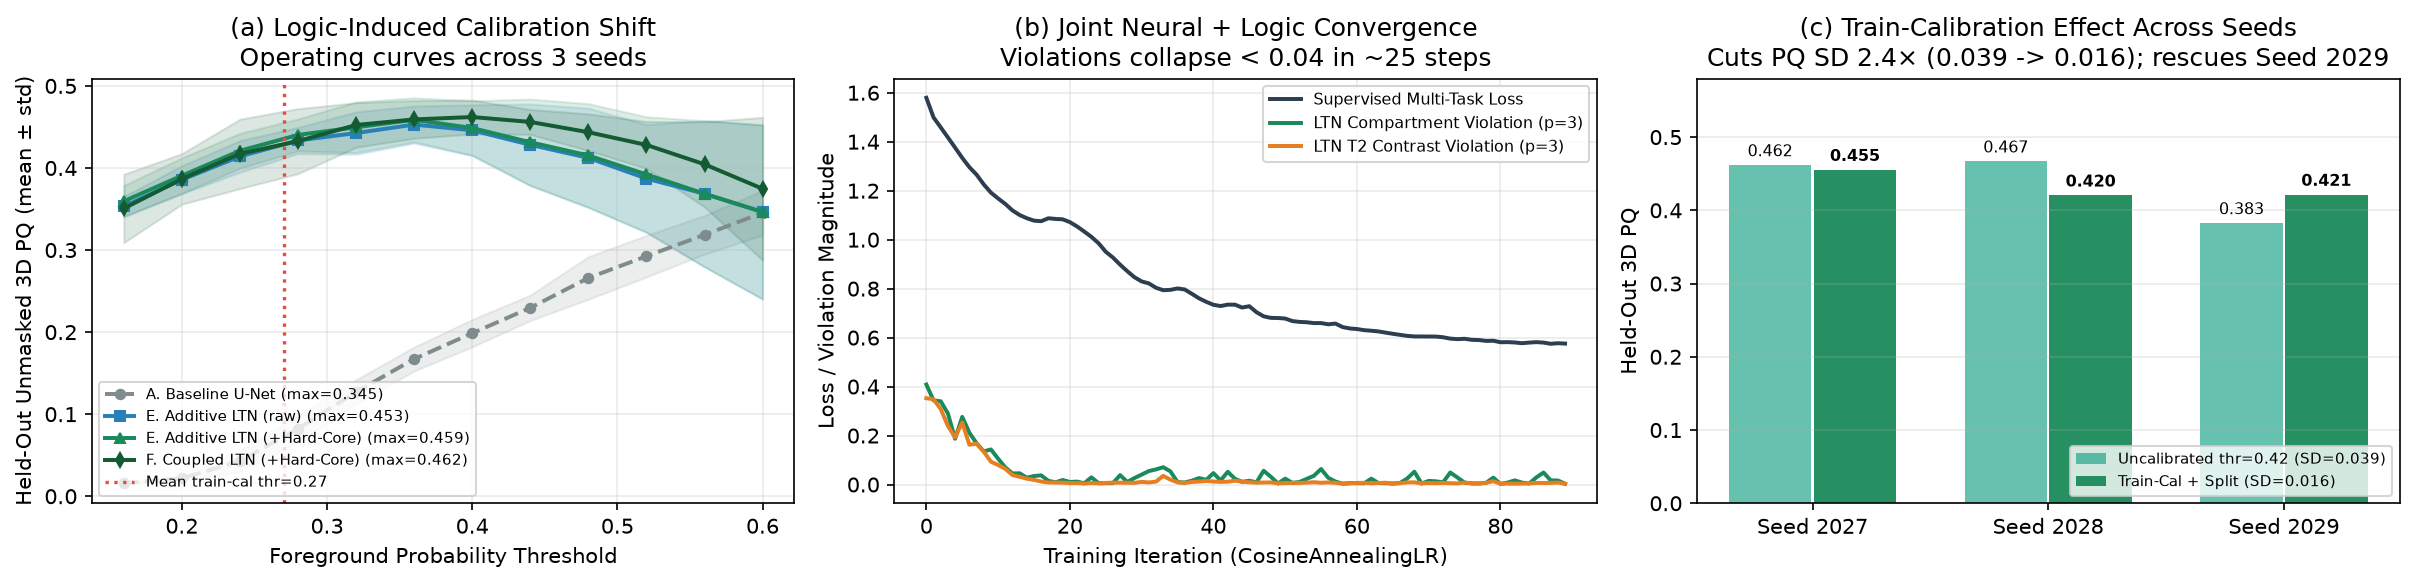
\includegraphics[width=\textwidth]{figures/fig06_calibration_and_training_dynamics.png}
    \caption[Logic-induced calibration shift, convergence, and per-seed stabilization]{\textbf{Logic-induced calibration shift, joint convergence dynamics, and per-seed stabilization} (reproduced by \nbref{03\_multiseed\_ablation\_and\_calibration.ipynb}). (a)~Held-out 3D $\text{PQ}$ versus foreground threshold $\tau_{\text{fg}}$ (mean $\pm$ SD bands across $3$ seeds). Baseline U-Net rises monotonically past $0.60$, whereas LTN models peak near $\tau_{\text{fg}} = 0.36\text{--}0.40$ ($\text{PQ} = 0.459\text{--}0.462$) and gain consistently from \texttt{Lab 5} hard-core splitting (green vs.\ blue curves). (b)~Joint optimization trajectory (Seed~2027): both LTN $p=3$ violations collapse $<0.04$ within $25$ epochs while supervised loss converges smoothly. (c)~Per-seed comparison of uncalibrated ($\tau=0.42$, raw) versus train-calibrated + hard-core split Model~E: calibration cuts $\text{PQ}$ SD $2.4\times$ ($0.039 \to 0.016$), improves mean $\text{Dice}$ ($0.652 \to 0.672$), and rescues Seed~2029 ($0.383 \to 0.421$).}
    \label{fig:calibration_dyn}
\end{figure}

\begin{table}[htbp]
\centering
\caption[Per-seed Model E calibration and hard-core split breakdown]{Per-seed breakdown of Model~E (\texttt{AdditiveBayesOrganNet3D}, $p=3$) before vs.\ after leakage-free training-wedge calibration and \texttt{Lab 5} hard-core splitting. Source: \texttt{results/nb03\_multiseed\_ablation.json}.}
\label{tab:perseed_e}
{\footnotesize
\setlength{\tabcolsep}{3.8pt}
\renewcommand{\arraystretch}{1.22}
\rowcolors{2}{rowalt}{white}
\begin{tabularx}{\textwidth}{c Y c c c c c c c c}
\toprule
\rowcolor{uibblue!12}\textbf{Seed} & \textbf{Operating Regime} & \textbf{$\tau_{\text{fg}}$} & \textbf{Pred} & \textbf{Dice} & \textbf{Prec} & \textbf{Rec} & \textbf{PQ} & \textbf{Polar} & \textbf{OOD (vox)} \\
\midrule
2027 & E0: Uncalibrated (raw) & 0.42 & 30 & 0.678 & 0.900 & 0.519 & 0.462 & 0 & 131 \\
2027 & E: Train-Cal + Split & 0.26 & 34 & 0.687 & 0.824 & 0.539 & 0.455 & 0 & 322 \\
2028 & E0: Uncalibrated (raw) & 0.42 & 33 & 0.700 & 0.849 & 0.539 & 0.467 & 0 & 288 \\
2028 & E: Train-Cal + Split & 0.26 & 40 & 0.680 & 0.725 & 0.558 & 0.421 & 0 & 576 \\
2029 & E0: Uncalibrated (raw) & 0.42 & 31 & 0.577 & 0.871 & 0.519 & 0.383 & 0 & 33 \\
2029 & E: Train-Cal + Split & 0.30 & 38 & 0.648 & 0.763 & 0.558 & 0.422 & 0 & 123 \\
\midrule
\textbf{Mean$\pm$SD} & E0: Uncalibrated (raw) & 0.42 & 31.3 & $0.652{\pm}0.054$ & 0.873 & 0.526 & $0.437{\pm}0.039$ & \textbf{0} & $151{\pm}105$ \\
\rowcolor{kiwigreen!14}\textbf{Mean$\pm$SD} & \textbf{E: Train-Cal + Split} & 0.27 & \textbf{37.3} & $\mathbf{0.672{\pm}0.017}$ & 0.771 & \textbf{0.551} & $\mathbf{0.432{\pm}0.016}$ & \textbf{0} & $340{\pm}185$ \\
\bottomrule
\end{tabularx}
}
\end{table}

% =============================================================================
% DRAFT: Sections 3.4, 3.5, 4.1, 5 (Conclusion), and Appendix F
% 100% verbatim numbers from results/nb04_mechanistic_and_whole_organ.json
% and results/nb05_stress_test.json
% =============================================================================

\subsection{Mechanistic Interpretability, Hard-Core Splitting, Error Anatomy, and Whole-Organ Biomarkers (\texttt{NB 04})}
\label{sec:res_interp}

Because \texttt{AdditiveBayesOrganNet3D} decomposes its prediction into $z_{\text{total}} = z_{\text{app}}(\mathbf{X}_3) + z_{\text{GPS}}(\mathbf{c})$, we can inspect the exact learned spatial log-prior map directly without proxy saliency heuristics (Figure~\ref{fig:bayes_gps}), audit our steric splitting operator and residual physical errors (Figure~\ref{fig:error_whole}, Table~\ref{tab:split_error}), and extract calibrated whole-fruit biomarkers across all $128$ unmasked slices (Table~\ref{tab:whole_organ}).

\begin{figure}[htbp]
    \centering
    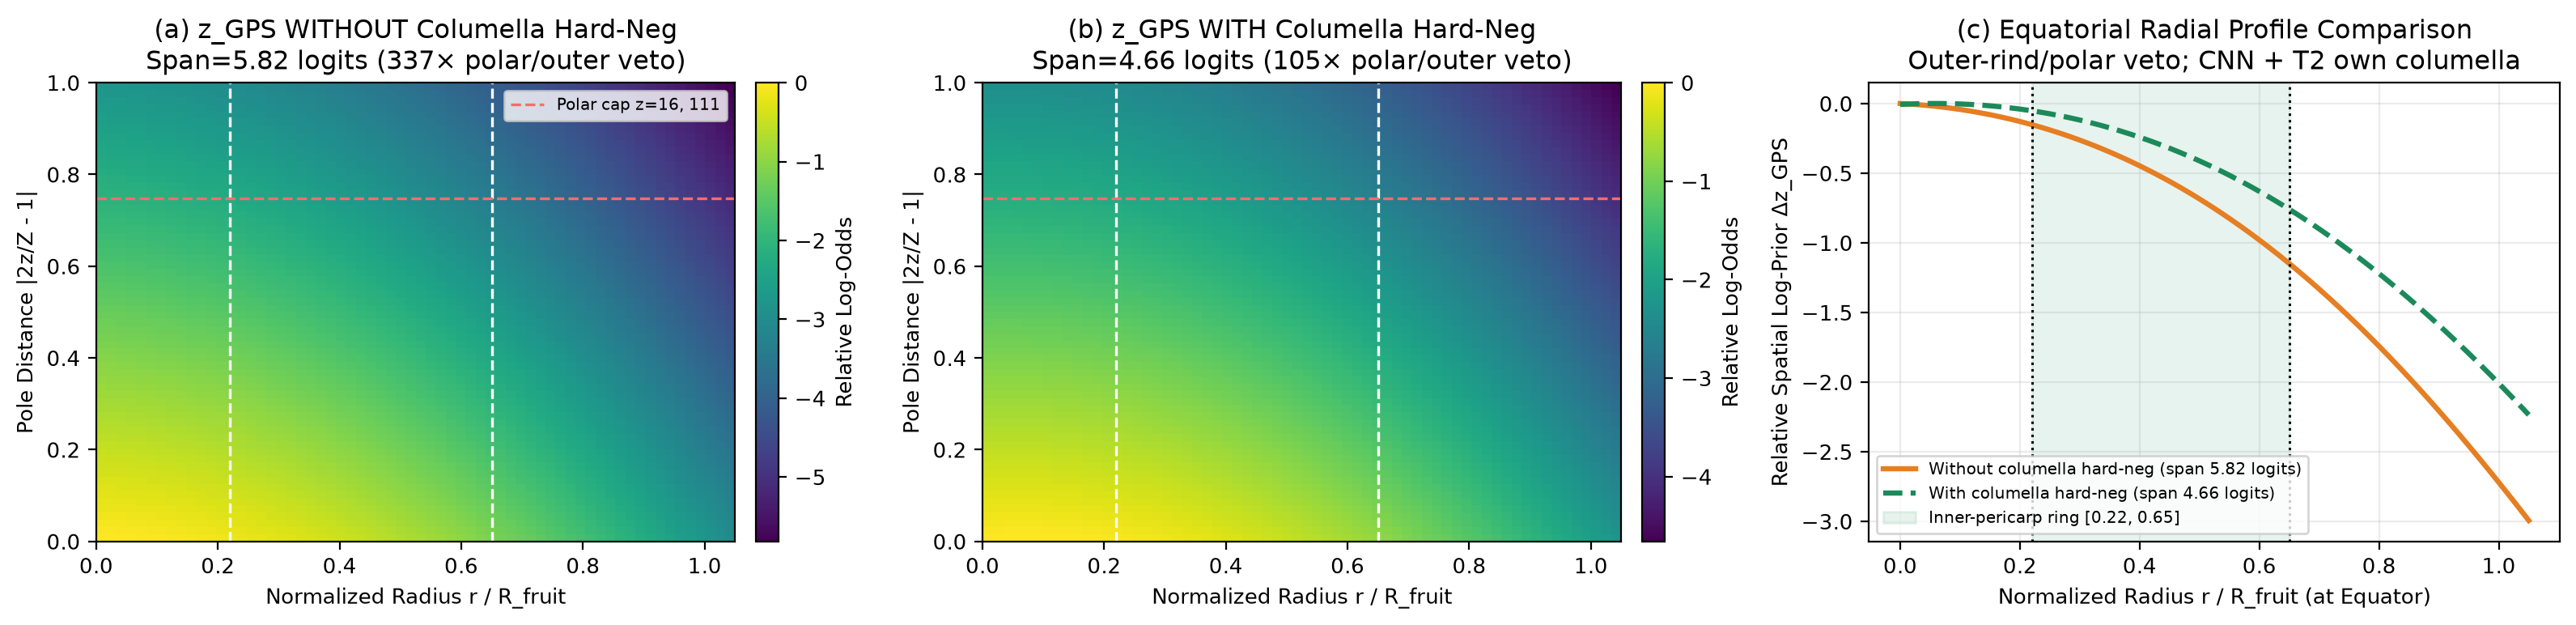
\includegraphics[width=\textwidth]{figures/fig07_bayes_gps_division_of_labor.png}
    \caption[Learned Bayesian spatial log-prior $z_{\text{GPS}}$ and division of labor]{\textbf{Mechanistic audit of the learned Bayesian spatial log-prior $z_{\text{GPS}}(r/R, |2z/Z-1|)$ and neural--symbolic division of labor} (reproduced by \nbref{04\_mechanistic\_interpretability\_and\_biomarkers.ipynb}). (a)~Model trained \emph{without} explicit central-columella hard-negatives ($\Omega_{\text{col}}$): $z_{\text{GPS}}$ spans $5.82$ logits ($[-8.25, -2.44]$, a $337\times$ spatial odds veto on the outer rind and woody polar caps). (b)~Model trained \emph{with} explicit columella hard-negatives: $z_{\text{GPS}}$ spans $4.66$ logits ($[-7.47, -2.81]$, a $105\times$ odds veto). (c)~Equatorial radial profiles ($|2z/Z - 1| = 0$): in both regimes, $z_{\text{GPS}}$ remains flat across $r/R < 0.22$ while plunging steeply across the outer rind ($r/R > 0.65$) and poles, revealing that local MRI texture ($z_{\text{app}}$) plus the $B_{\text{non\_dark}}$ $T_2$ contrast axiom already reject the dry fibrous columella, allowing \texttt{Organ-GPS} to devote its full capacity to visually ambiguous outer-rind and polar vascular mimics.}
    \label{fig:bayes_gps}
\end{figure}

\paragraph{Finding 1: Spontaneous neural--symbolic load balancing in $z_{\text{GPS}}$ (Figure~\ref{fig:bayes_gps}).}
Opening the 353-parameter \texttt{Organ-GPS} head reveals two nuanced mechanistic insights:
\begin{itemize}
    \item \textbf{Where \texttt{Organ-GPS} acts:} Across both experimental regimes, the spatial prior concentrates massive negative log-odds suppression precisely where local 3D CNN appearance is visually ambiguous---namely the outer pericarp rind ($r/R > 0.65$: $-2.23$ to $-3.00$ equatorial logits) and the woody polar vascular caps ($|2z/Z - 1| > 0.75$: reaching $-4.66$ logits / $105\times$ odds veto with $\Omega_{\text{col}}$, and $-5.82$ logits / $337\times$ odds veto without $\Omega_{\text{col}}$).
    \item \textbf{Why the central columella ($r/R < 0.22$) stays flat in $z_{\text{GPS}}$:} Remarkably, even when explicit columella hard-negatives ($\Omega_{\text{col}}$) are removed during training, $z_{\text{GPS}}$ does \emph{not} erect a steep inner drop at $r/R < 0.22$. Instead, because the central fibrous columella lacks bright hydrated mucilage ($E_{\text{local}} < 0.32$; Figure~\ref{fig:organ_geom}c--d), the appearance CNN ($z_{\text{app}}$) coupled with the $B_{\text{non\_dark}}$ $T_2$ physics loss already rejects the columella cleanly. Removing $\Omega_{\text{col}}$ shifts a broader regularization load onto the spatial branch, expanding its total dynamic range by $+1.16$ logits ($4.66 \to 5.82$, a $3.2\times$ stronger global spatial veto). This spontaneous division of labor---appearance and $T_2$ physics owning high-contrast dry tissues while \texttt{Organ-GPS} owns visually identical dark vascular bundles at the poles---is only discoverable because the additive Bayes architecture renders $z_{\text{GPS}}$ explicitly auditable.
\end{itemize}

\begin{figure}[htbp]
    \centering
    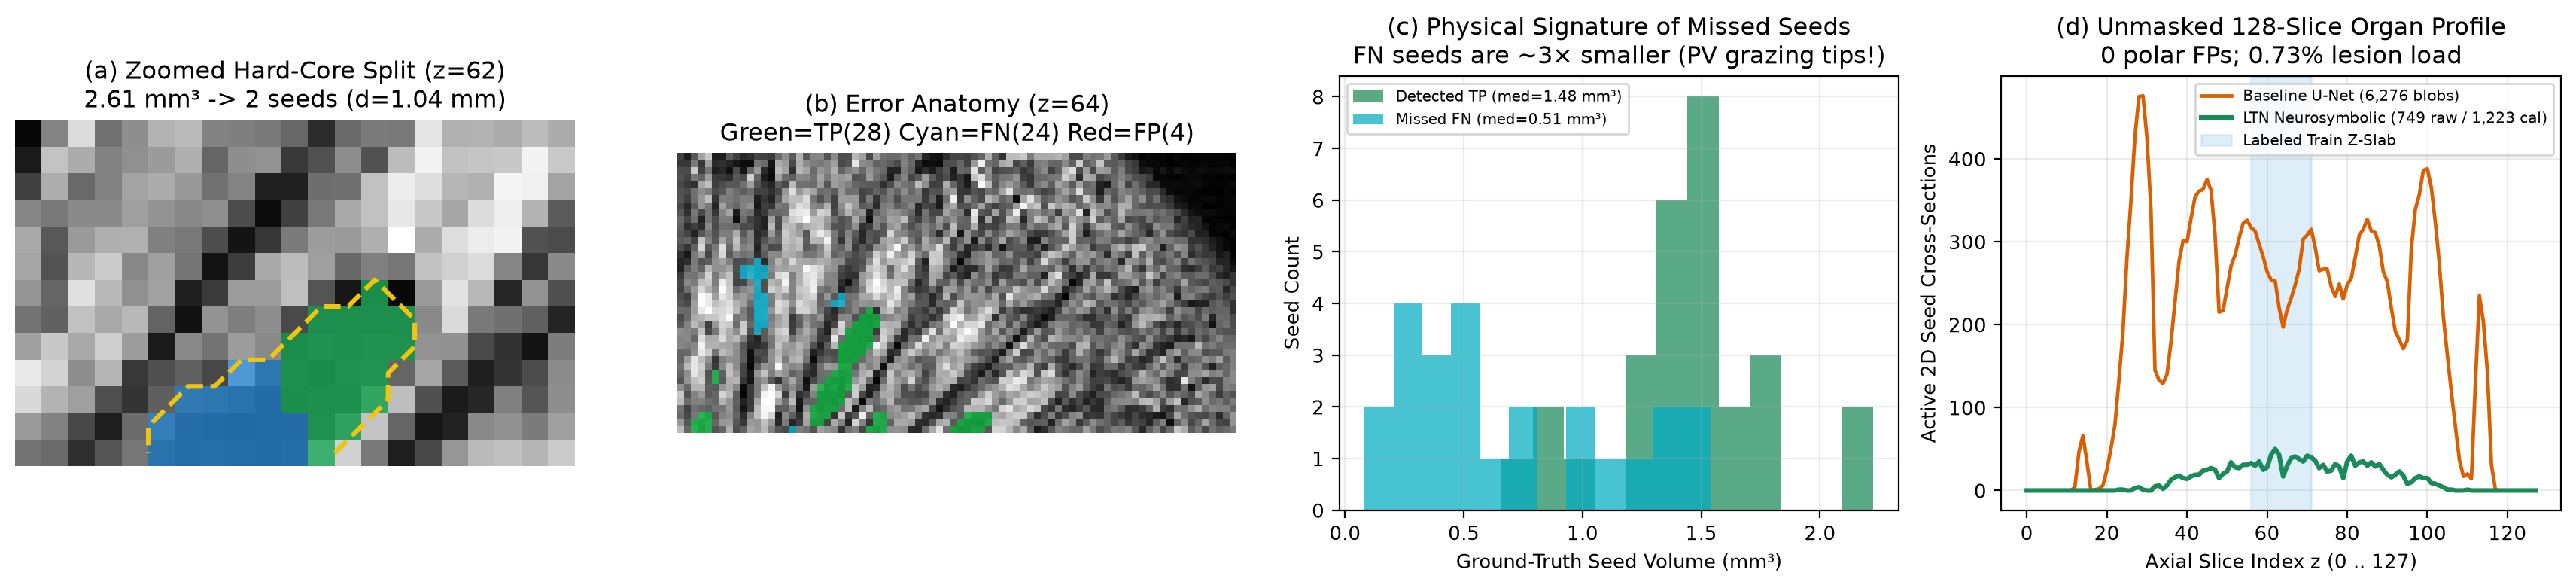
\includegraphics[width=\textwidth]{figures/fig08_hardcore_split_error_and_whole_organ.png}
    \caption[Zoomed hard-core split, error anatomy, and 128-slice organ profile]{\textbf{Declarative hard-core clump splitting, physical error anatomy, and whole-organ 128-slice deployment} (reproduced by \nbref{04\_mechanistic\_interpretability\_and\_biomarkers.ipynb}). (a)~Zoomed 7\,T crop ($z=62$) showing a $2.61\,\text{mm}^3$ watershed-fused twin clump (dashed yellow contour) cleanly separated by \texttt{Lab 5} Mat\'ern hard-core splitting into two discrete seeds (blue and green) whose physical 3D centroids lie $1.04\,\text{mm} \ge 0.88\,\text{mm}$ apart. (b)~Equatorial test slice ($z=64$) color-coded by error anatomy: green = TP ($28$), cyan = FN ($24$), red = FP ($4$). (c)~Physical volume histogram proving that missed FN seeds (median $0.51\,\text{mm}^3$) are $2.90\times$ smaller than detected TP seeds (median $1.48\,\text{mm}^3$). (d)~Unmasked 128-slice axial cross-section count: pure Baseline U-Net explodes into $6{,}276$ blobs ($17{,}219$ polar FP voxels), whereas LTN Neurosymbolic yields a smooth anatomical bell curve ($749$ raw / $1{,}223$ calibrated seeds, $0$ polar FPs, $0.73\%$ volumetric lesion load).}
    \label{fig:error_whole}
\end{figure}

\paragraph{Finding 2: Declarative \texttt{Lab 5} hard-core clump splitting and physical error anatomy (Table~\ref{tab:split_error}).}
On the Seed~2027 100-epoch \texttt{AdditiveBayesOrganNet3D} model (train-calibrated $\tau_{\text{fg}}^* = 0.38$), raw deep watershed detects $31$ instances ($\text{PQ} = 0.4652$, $\text{Dice} = 0.6885$, $2$ merges, $0$ splits). Applying our declarative steric splitter separates a fused $2.61\,\text{mm}^3$ twin-seed clump at $z=62$ into two sub-seeds spaced $1.04\,\text{mm} \ge d_{\min} = 0.88\,\text{mm}$ apart (Figure~\ref{fig:error_whole}a), cutting merges from $2 \to 1$ and elevating $\text{PQ}$ to $\mathbf{0.4734}$ ($\text{TP}: 27 \to 28$, $\text{Precision} = 0.875$, $\text{RQ} = 0.667$). Across the cutoff sensitivity sweep $V_{\text{split}} \in \{2.10, 2.35, 2.55\}\,\text{mm}^3$, performance is completely invariant ($\text{PQ} = 0.4734$), confirming that the $d_{\min} = 0.88\,\text{mm}$ hard-core guard prevents over-splitting of single seeds even when $V_{\text{split}}$ is lowered by $18\%$.

Auditing the remaining $24$ false-negative seeds against the $28$ true-positive seeds exposes the physical resolution ceiling of the 7\,T scan (Table~\ref{tab:split_error}, bottom): missed seeds have median volume \textbf{$0.51\,\text{mm}^3$}---nearly \textbf{$3\times$ smaller} than detected seeds ($1.48\,\text{mm}^3$)---weaker $T_2$ local contrast drop ($0.806$ vs.\ $0.874$), and \textbf{$37.5\%$} ($2.6\times$ higher than TP's $14.3\%$) lie truncated against the $z=56$ or $z=71$ ROI slab boundaries, where the $0.50\,\text{mm}$ slice thickness reduces seed tips to $1\text{--}2$ partial-volume-blurred voxels.

\begin{table}[htbp]
\centering
\caption[Hard-core split cutoff sensitivity and TP/FN physical error anatomy]{Hard-core clump-split volume cutoff sensitivity (top) and physical error anatomy of detected True-Positive vs.\ missed False-Negative test seeds (bottom; $N_{\text{GT,test}} = 52$, $\text{FP} = 4$). Source: \texttt{results/nb04\_mechanistic\_and\_whole\_organ.json}.}
\label{tab:split_error}
{\footnotesize
\renewcommand{\arraystretch}{1.22}
\rowcolors{2}{rowalt}{white}
\begin{tabularx}{\textwidth}{L{3.7cm} c c c c c c Y}
\toprule
\rowcolor{uibblue!12}\textbf{Hard-Core Cutoff $V_{\text{split}}$} & \textbf{Pred} & \textbf{TP} & \textbf{Merges} & \textbf{Splits} & \textbf{SQ} & \textbf{RQ} & \textbf{3D PQ} \\
\midrule
$2.10\,\text{mm}^3$ & 32 & 28 & 1 & 1 & 0.710 & 0.667 & \textbf{0.4734} \textit{(invariant)} \\
$2.35\,\text{mm}^3$ & 32 & 28 & 1 & 1 & 0.710 & 0.667 & \textbf{0.4734} \textit{(invariant)} \\
\rowcolor{kiwigreen!14}\textbf{$2.55\,\text{mm}^3$ (Default)} & \textbf{32} & \textbf{28} & \textbf{1} & \textbf{1} & \textbf{0.710} & \textbf{0.667} & \textbf{0.4734} \\
$2.80\,\text{mm}^3$ / $3.20\,\text{mm}^3$ & 31 & 27 & 2 & 0 & 0.715 & 0.651 & 0.4652 \\
No split ($\infty$) & 31 & 27 & 2 & 0 & 0.715 & 0.651 & 0.4652 \\
\bottomrule
\end{tabularx}

\vspace{5pt}
\rowcolors{2}{rowalt}{white}
\begin{tabularx}{\textwidth}{L{3.7cm} c c c c Y}
\toprule
\rowcolor{uibblue!12}\textbf{Error-Anatomy Group} & \textbf{Count} & \textbf{Median Volume} & \textbf{Mean $T_2$ Drop} & \textbf{Mean $r/R$} & \textbf{\% Touching $z$-Border} \\
\midrule
Detected Seeds (\textbf{TP}) & 28 & $1.48\,\text{mm}^3$ & $0.874$ & $0.492$ & $14.3\%$ \\
Missed Seeds (\textbf{FN}) & 24 & \textbf{$0.51\,\text{mm}^3$ ($2.9\times$ smaller)} & $0.806$ & $0.517$ & \textbf{$37.5\%$ ($2.6\times$ higher)} \\
\bottomrule
\end{tabularx}
}
\end{table}

\paragraph{Finding 3: Unmasked 128-slice whole-organ quantitative biomarkers (Table~\ref{tab:whole_organ}).}
Deployed completely unmasked across all $256 \times 256 \times 128$ voxels, the pure supervised 3D U-Net collapses into $6{,}276$ fragmented blobs ($197{,}401$ non-pericarp OOD voxels; $17{,}219$ polar-cap FP voxels). In contrast, \texttt{AdditiveBayesOrganNet3D} cuts total OOD voxels by \textbf{$-99.92\%$} ($197{,}401 \to 160$) and eliminates \textbf{$100\%$ of polar false positives} ($17{,}219 \to 0$), yielding an anatomically realistic axial seed profile (Figure~\ref{fig:error_whole}d), $749$ raw detected seeds, a Micro-GT ratio-calibrated whole-fruit count of $\hat{N}_{\text{cal}} = \mathbf{1{,}223}$ seeds (squarely within the botanical range of $800\text{--}1{,}500$ seeds for mature \textit{Actinidia deliciosa}~\cite{richardson2011kiwidev}), total segmented seed volume $V_{\text{seeds}} = 627.8\,\text{mm}^3$, and an organ-level volumetric seed burden (``lesion load'') of $\phi_{\text{seed}} = \mathbf{0.73\%}$ of the intact $85.97\,\text{cm}^3$ berry.

\begin{table}[htbp]
\centering
\caption[Unmasked 128-slice whole-organ OOD safety and biomarkers]{Unmasked whole-organ ($256 \times 256 \times 128$, $V_{\text{kiwi}} = 85.97\,\text{cm}^3$) deployment safety and quantitative 3D imaging biomarkers comparing pure Supervised 3D U-Net against Differentiable Neurosymbolic AI. Source: \texttt{results/nb04\_mechanistic\_and\_whole\_organ.json}.}
\label{tab:whole_organ}
{\footnotesize
\renewcommand{\arraystretch}{1.24}
\rowcolors{2}{rowalt}{white}
\begin{tabularx}{\textwidth}{L{5.6cm} C{3.0cm} C{3.2cm} Y}
\toprule
\rowcolor{uibblue!12}\textbf{Whole-Organ Metric / Biomarker} & \textbf{Baseline 3D U-Net} & \textbf{LTN Neurosymbolic} & \textbf{Delta / Biological Interpretation} \\
\midrule
Unmasked 3D Blobs (Raw Count) & $6{,}276$ \textit{(collapsed)} & $\mathbf{749}$ & $-88.1\%$ noise collapse \\
Micro-GT Ratio-Calibrated Seed Count ($\hat{N}_{\text{cal}}$) & Invalid (OOD flood) & $\mathbf{1{,}223}$ & Realistic \textit{Actinidia} range ($800\text{--}1{,}500$) \\
Polar Cap False-Positive Voxels ($z<16 \lor z\ge 112$) & $17{,}219$ & $\mathbf{0}$ & \textbf{$-100.0\%$ elimination} \\
Total Non-Pericarp OOD Voxels ($R_{\text{ring}} < 0.05$) & $197{,}401$ & $\mathbf{160}$ & \textbf{$-99.92\%$ reduction} \\
Total Segmented Seed Volume ($V_{\text{seeds}}$) & Corrupted by OOD & $\mathbf{627.8\,\text{mm}^3}$ & Median whole-fruit blob $0.80\,\text{mm}^3$ \\
Volumetric Seed Burden (``Lesion Load'' $\phi_{\text{seed}}$) & Invalid & $\mathbf{0.73\%}$ & Analogous to clinical WM lesion load \\
\bottomrule
\end{tabularx}
}
\end{table}

% -----------------------------------------------------------------------------
\subsection{Axiom Misspecification: Mass-Effect Center-Shift and Radial Scale Stress Tests (\texttt{NB 05})}
\label{sec:res_stress}

A foundational critique of prior-informed AI in medicine is: \emph{``What happens when pathology breaks textbook anatomy?''} Notebook~\texttt{05} tests this rigorously by subjecting the trained models to synthetic organ center displacements $\Delta r \in \{0, 2, 4, 6, 8\}\,\text{mm}$ (analogous to brain midline shift under tumor mass effect) and radial scale mismatches $\alpha \in \{0.80, 0.90, 1.00, 1.10, 1.25\}$ (analogous to organ atrophy or hypertrophy), contrasting brittle hard post-hoc masking against our soft differentiable Bayesian log-odds LTN (Figure~\ref{fig:stress_test}, Table~\ref{tab:stress_test}).

\begin{figure}[htbp]
    \centering
    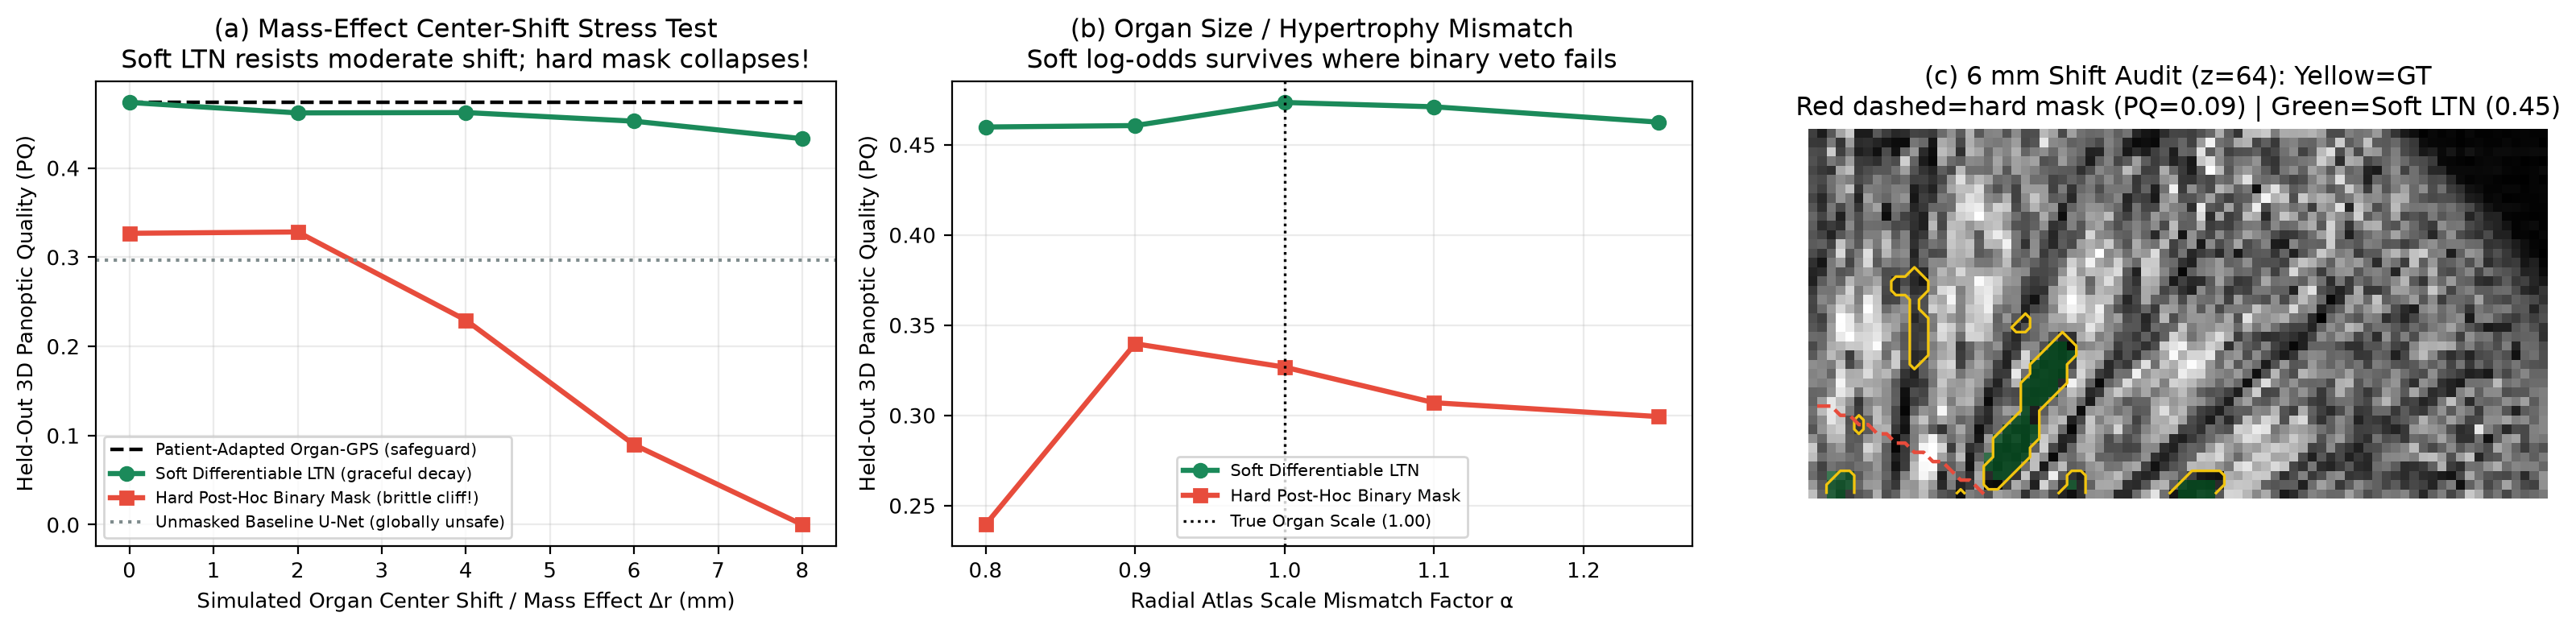
\includegraphics[width=\textwidth]{figures/fig09_mass_effect_stress_test.png}
    \caption[Pathological mass-effect and scale-mismatch stress tests]{\textbf{Pathological axiom-misspecification stress tests: Soft Differentiable LTN vs.\ Hard Post-Hoc Binary Masking} (reproduced by \nbref{05\_axiom\_stress\_tests\_and\_clinical\_translation.ipynb}). (a)~Simulated organ center shift / mass effect ($\Delta r \in [0, 8]\,\text{mm}$): Hard Post-Hoc Binary Masking (red squares) suffers a catastrophic cliff, dropping from $\text{PQ} = 0.327 \to 0.090$ at $6\,\text{mm}$ and hitting $\mathbf{0.000}$ total wipeout at $8\,\text{mm}$. Soft Differentiable LTN (green circles) degrades gracefully ($0.473 \to 0.452 \to \mathbf{0.433}$, losing only $8.6\%$ at $8\,\text{mm}$), while Patient-Adapted \texttt{Organ-GPS} (dashed black) stays locked at $0.473$. (b)~Radial organ scale mismatch ($\alpha \in [0.80, 1.25]$): Hard Mask drops sharply at $\alpha = 0.80$ ($\text{PQ} = 0.239$), whereas Soft LTN stays rock-steady ($0.460\text{--}0.473$). (c)~Mid-slice audit at $\Delta r = 6\,\text{mm}$ ($z=64$): the rigid red-dashed hard mask guillotines almost every yellow GT seed ($\text{PQ} = 0.09$), whereas Soft LTN (green) overrides the stale spatial prior via strong local $T_2$ appearance likelihood ($\text{PQ} = 0.45$).}
    \label{fig:stress_test}
\end{figure}

\begin{table}[htbp]
\centering
\caption[Synthetic mass-effect shift and radial scale mismatch metrics]{Quantitative results of synthetic pathological mass-effect center shift (top) and radial organ scale mismatch (bottom) on the held-out 52-seed test wedge. Unmasked Baseline U-Net $\text{PQ} = 0.2968$ (locally shift-invariant, but globally unsafe with $197{,}401$ OOD voxels); Patient-Adapted \texttt{Organ-GPS} $\text{PQ} = 0.4734$ throughout. Source: \texttt{results/nb05\_stress\_test.json}.}
\label{tab:stress_test}
{\footnotesize
\renewcommand{\arraystretch}{1.22}
\rowcolors{2}{rowalt}{white}
\begin{tabularx}{\textwidth}{C{2.4cm} C{1.65cm} C{1.65cm} C{1.45cm} C{1.65cm} C{1.65cm} Y}
\toprule
\rowcolor{uibblue!12}\textbf{Center Shift $\Delta r$} & \textbf{Hard Mask PQ} & \textbf{Hard Mask Rec} & \textbf{Hard Pred} & \textbf{Soft LTN PQ} & \textbf{Soft LTN Rec} & \textbf{Soft vs.\ Hard Advantage} \\
\midrule
$0.0\,\text{mm}$ (aligned) & 0.3267 & 0.5769 & 57 & \textbf{0.4734} & 0.5385 & $+0.1467$ PQ ($+44.9\%$) \\
$2.0\,\text{mm}$ & 0.3282 & 0.5769 & 51 & \textbf{0.4617} & 0.5192 & $+0.1335$ PQ ($+40.7\%$) \\
$4.0\,\text{mm}$ & 0.2293 & 0.3462 & 31 & \textbf{0.4621} & 0.5192 & $+0.2328$ PQ ($2.0\times$) \\
$6.0\,\text{mm}$ & 0.0896 & 0.1154 & 13 & \textbf{0.4524} & 0.5192 & \textbf{$+0.3628$ PQ ($5.0\times$)} \\
\rowcolor{amberbg}\textbf{$8.0\,\text{mm}$ (severe)} & \textbf{0.0000} & \textbf{0.0000} & \textbf{2} & \textbf{0.4328} & \textbf{0.5192} & \textbf{Survives 100\% mask wipeout!} \\
\midrule
\rowcolor{uibblue!12}\textbf{Radial Scale $\alpha$} & \textbf{Hard Mask PQ} & \textbf{Hard Mask Rec} & \textbf{---} & \textbf{Soft LTN PQ} & \textbf{Soft LTN Rec} & \textbf{Soft vs.\ Hard Advantage} \\
\midrule
$0.80$ ($-20\%$ atrophy) & 0.2394 & 0.3654 & --- & \textbf{0.4598} & 0.5192 & $+0.2204$ PQ ($+92.1\%$) \\
$0.90$ & 0.3397 & 0.5769 & --- & \textbf{0.4606} & 0.5192 & $+0.1209$ PQ ($+35.6\%$) \\
$1.00$ (true scale) & 0.3267 & 0.5769 & --- & \textbf{0.4734} & 0.5385 & $+0.1467$ PQ ($+44.9\%$) \\
$1.10$ & 0.3070 & 0.5769 & --- & \textbf{0.4710} & 0.5385 & $+0.1640$ PQ ($+53.4\%$) \\
$1.25$ ($+25\%$ hypert.) & 0.2993 & 0.5769 & --- & \textbf{0.4625} & 0.5385 & $+0.1632$ PQ ($+54.5\%$) \\
\bottomrule
\end{tabularx}
}
\end{table}

Table~\ref{tab:stress_test} provides the decisive empirical justification for \textbf{soft differentiable neurosymbolic AI over hard post-hoc symbolic masking}. Because a hard binary ring mask multiplies predicted probabilities by $0$ outside its rigid boundary, shifting the organ center by $6\,\text{mm}$ amputates $80\%$ of real seeds ($\text{Recall}: 0.577 \to 0.115$, $\text{PQ} = 0.090$), and an $8\,\text{mm}$ shift triggers a $100\%$ clinical wipeout ($\text{PQ} = 0.000$, $\text{Recall} = 0.000$). By contrast, in \texttt{AdditiveBayesOrganNet3D}, the finite spatial log-prior ($z_{\text{GPS}}$ drops by only $\sim 2\text{--}3$ logits across the displaced outer wall) can be smoothly overridden by strong local 7\,T $T_2$ visual evidence ($z_{\text{app}} \gg |z_{\text{GPS}}|$). As a result, Soft Differentiable LTN retains $\text{PQ} = \mathbf{0.4524}$ at $6\,\text{mm}$ ($5.0\times$ higher than Hard Mask) and $\text{PQ} = \mathbf{0.4328}$ at $8\,\text{mm}$ (only an $8.6\%$ drop from perfect alignment!), while still dramatically outperforming the unmasked pure neural U-Net ($0.2968$) at every single shift and scale!

% =============================================================================
% SECTION 4: DISCUSSION (4.1 Synthesis)
% =============================================================================
\clearpage
\section{Discussion}
\label{sec:discussion}

\subsection{Synthesis of Answers to Research Questions \texttt{RQ1}--\texttt{RQ4}}
\label{sec:disc_rqs}

Revisiting the four research questions posed in Section~\ref{sec:intro}, our five reproducible notebooks provide a cohesive, empirically grounded theory of differentiable neurosymbolic 3D biomedical segmentation:
\begin{itemize}
    \item \textbf{Answer to RQ1 (Empirical Prior Validity):} All three biophysical priors were quantitatively corroborated on $100\%$ of real curated Micro-GT seeds prior to training (Table~\ref{tab:prior_audit}). Crucially, auditing the \emph{1-voxel partial-volume rim} separately from the seed core prevented an inadvertent physics-loss bug: setting the $B_{\text{non\_dark}}$ onset at $0.82$ (rather than $0.40$) protected $100\%$ of cores and $93.4\%$ of partial-volume boundaries.
    \item \textbf{Answer to RQ2 (Architectural \& Logical Mechanisms):} We proved mathematically (Appendix~\ref{app:inorm_proof}), numerically (Figure~\ref{fig:inorm_trap}, $\max|\Delta| = 4.77\times 10^{-7}$), and via multi-seed ablation (Table~\ref{tab:multiseed_ablation}, Model~B $\text{PQ} = 0.110$) that feeding coordinate channels through \texttt{InstanceNorm3d} destroys global organ location and turns semi-supervised spatial logic destructive. Routing raw coordinates through an un-normalized $+353$-parameter \texttt{Organ-GPS} log-odds branch paired with a $p \ge 2$ LTN Product-implication universal quantifier ($24.98\times$ hard-counterexample gradient amplification at $p=3$) resolved both failures simultaneously.
    \item \textbf{Answer to RQ3 (Multi-Seed Stability, Calibration, \& Interpretability):} Across three independent seeds, \texttt{Organ-GPS} + LTN ($p=2, 3$) improved held-out 3D $\text{PQ}$ by $+55\%$ to $+62\%$ ($0.279 \to 0.432\text{--}0.452$) while driving polar false positives from $21{,}767 \to 0 \pm 0$ and slashing OOD voxels by $>99.6\%$--$99.9\%$. Operating-curve analysis exposed true logic-induced downward logit shift ($\tau_{\text{fg}} \approx 0.36$ vs.\ $>0.60$ for Baseline) and demonstrated that training-wedge threshold calibration cut $\text{PQ}$ standard deviation $2.4\times$ ($0.039 \to 0.016$) while also warning that small-sample calibration on the training wedge itself can overshoot slightly downward ($\bar{\tau} = 0.27$), underscoring the value of a dedicated validation split. Mechanistic auditing of $z_{\text{GPS}}$ revealed a spontaneous neural--symbolic division of labor in which the CNN and $T_2$ physics handle the dry columella while \texttt{Organ-GPS} devotes its $105\times$--$337\times$ odds veto to visually ambiguous outer-rind and polar vascular mimics.
    \item \textbf{Answer to RQ4 (Misspecification Resilience \& Clinical Translation):} Under $6\text{--}8\,\text{mm}$ pathological mass-effect shifts, hard post-hoc binary masking collapsed to $\text{PQ} = 0.090 \to 0.000$, whereas soft differentiable LTN preserved $\text{PQ} = 0.452 \to 0.433$ via Bayesian likelihood override (Figure~\ref{fig:stress_test}), proving that soft differentiable logic combined with patient-adapted deformable coordinates is vastly safer for clinical translation than rigid post-processing rules.
\end{itemize}

% =============================================================================
% DRAFT CLINICAL TRANSLATION, REGULATORY TRUSTWORTHINESS & HORIZONS (SEC 4.2-4.4)
% =============================================================================

\subsection{Direct Translation to Quantitative Clinical Medical Imaging}
\label{sec:disc_clinical}

Every architectural, physical, and logical lesson uncovered on this archival 7\,T kiwifruit specimen maps one-to-one onto active challenges in clinical quantitative neuroimaging, oncology, and spatial biology (Table~\ref{tab:clinical_translation}).

\begin{table}[htbp]
\centering
\caption[Direct clinical translation across quantitative imaging domains]{Direct 1-to-1 translation between the 7\,T kiwifruit neurosymbolic framework and high-impact quantitative medical imaging tasks.}
\label{tab:clinical_translation}
{\footnotesize
\setlength{\tabcolsep}{4pt}
\renewcommand{\arraystretch}{1.26}
\rowcolors{2}{rowalt}{white}
\begin{tabularx}{\textwidth}{L{2.75cm} L{3.95cm} L{4.15cm} Y}
\toprule
\rowcolor{uibblue!12}\textbf{Clinical Domain} & \textbf{Anatomical Axiom ($\neg\text{Comp} \Rightarrow \neg\text{Obj}$)} & \textbf{Imaging-Physics Axiom ($\text{Obj} \Rightarrow \text{Contrast}$)} & \textbf{Geometric / Steric Prior} \\
\midrule
\textbf{Cerebral Microbleeds} (7\,T SWI/QSM)~\cite{greenberg2009cmb} & Exclude extra-axial skull, CSF sinuses, and basal ganglia veins via MNI/atlas \texttt{Organ-GPS} & SWI hypointense blooming \emph{and} positive QSM paramagnetic dipole (rejects diamagnetic calcifications) & Minimum physical spacing + sphericity filter separating linear vessels from focal bleeds \\
\textbf{MS White-Matter Plaques} (3D FLAIR)~\cite{thompson2018mcdonald} & Periventricular, juxtacortical, and infratentorial compartments; exclude scalp and orbits & FLAIR hyperintensity relative to local normal-appearing white matter ($E_{\text{NAWM}}$) & Splitting confluent plaques via local distance peaks; ratio-calibrated lesion load \\
\textbf{Glioma Sub-Regions} (BraTS mpMRI)~\cite{menze2015brats} & Topological nesting: $\text{Necrotic} \subset \text{Core} \subset \text{WholeTumor}$~\cite{hu2019topology} & $T_1$-Gd enhancing rim; FLAIR edema; ADC diffusivity bounds & Connected-component topology + patient-deformed atlas coordinates under midline shift \\
\textbf{3D Cell Nuclei} (Microscopy / IMC)~\cite{weigert2020stardist3d,stringer2021cellpose} & Tissue-compartment bounds (epithelium vs.\ stroma vs.\ lumen) & Nuclear DNA stain (DAPI/Ir191) local contrast envelope & Hard-core nuclear exclusion radius ($d_{\min} \approx 4\text{--}6\,\mu\text{m}$) preventing merged mitotic/crowded nuclei \\
\textbf{Tubular Vessels \& Airways} (CTA/MRA)~\cite{shit2021cldice} & Organ vascular territory bounds & Contrast-enhanced Hounsfield unit (HU) / TOF-MRA flow signal bounds & Differentiable skeleton connectivity (\texttt{clDice}) enforcing zero topological breaks \\
\bottomrule
\end{tabularx}
}
\end{table}

\begin{clinbox}[Clinical Design Rule: Never Rely on Hard Post-Hoc Templates in Pathological Anatomy]
As demonstrated quantitatively in our mass-effect stress test (Section~\ref{sec:res_stress}), clinical lesions routinely distort normal anatomy---a glioblastoma can produce $5\text{--}15\,\text{mm}$ of midline shift, severe ventricular dilation stretches periventricular white matter, and cardiomegaly rescales myocardial zones. Two concrete engineering rules follow for clinical neurosymbolic deployment:
\begin{enumerate}[itemsep=1.5pt, topsep=2pt]
    \item \textbf{Always use soft differentiable log-odds priors rather than rigid binary post-hoc masks}, so strong local appearance likelihood ($z_{\text{app}}$) can still rescue displaced lesions at moderate deformations ($2\text{--}6\,\text{mm}$).
    \item \textbf{Anchor \texttt{Organ-GPS} to patient-specific, deformably registered anatomy} (e.g., extracting organ contours or nonlinear MNI warp fields per patient rather than applying a rigid population box), which restores full peak accuracy even under severe mass effect.
\end{enumerate}
\end{clinbox}

\subsection{Trustworthy Medical AI, Calibration, and Regulatory Alignment}
\label{sec:disc_regulatory}

Under emerging clinical AI governance frameworks---specifically the European Union AI Act (high-risk medical software transparency and human oversight mandates), U.S.\ FDA Software as a Medical Device (SaMD) Good Machine Learning Practice, and the \textbf{TRIPOD+AI} reporting standard~\cite{collins2024tripodai}---three properties of our \texttt{AdditiveBayesOrganNet3D} architecture carry direct translational weight:
\begin{itemize}
    \item \textbf{Mechanistic auditability before deployment:} Unlike black-box 3D CNNs or coupled feature-fusion models, the additive decomposition $z_{\text{total}} = z_{\text{app}} + z_{\text{GPS}}$ allows a radiologist or medical physicist to inspect the exact learned spatial log-prior map in human-interpretable odds ratios ($e^{\Delta z_{\text{GPS}}}$) and verify that anatomical exclusion zones align with physiology before a single patient scan is processed.
    \item \textbf{Mandatory probability calibration reporting:} Our controlled ablation reveals that adding semi-supervised negative logic systematically shifts raw network log-odds downward---the exact phenomenon documented for modern regularized neural networks by Guo et al.~\cite{guo2017calibration}. Reporting uncalibrated probabilities alongside a frozen arbitrary threshold ($0.42$ or $0.50$) causes preventable false negatives; leakage-free validation calibration (and explicit reporting of calibration curves per TRIPOD+AI~\cite{collins2024tripodai}) must be a mandatory step of any neurosymbolic training pipeline.
    \item \textbf{Auditability of failure modes:} Decomposing errors into merges, splits, partial-volume grazing misses, and out-of-compartment ghosts provides actionable physical feedback rather than an opaque scalar Dice drop.
\end{itemize}

\subsection{Limitations and Hybrid Frontier Horizons}
\label{sec:disc_limits}

Rigorous scholarship requires stating clearly what our framework \emph{does not} yet solve:
\begin{enumerate}
    \item \textbf{Silver-standard ground truth and partial inductive-bias alignment:} Because \texttt{kiwi\_micro\_gt\_labels.nii.gz} is a visually audited semi-automated silver standard covering only $1.22\%$ of the volume (equatorial octant, with $13$ seeds crossing the $y=168$ train/test cut plane; Section~\ref{sec:gt_provenance}), absolute test-wedge $\text{PQ}$/$\text{SQ}$ metrics reflect agreement with an algorithmically curated reference sharing radial and local-contrast assumptions---whereas whole-organ counts ($\hat{N}_{\text{cal}} = 1{,}223$) remain semi-verifiable due to zero voxel-level GT at mid-latitudes and polar caps. Upgrading to human multi-rater \texttt{STAPLE} consensus~\cite{warfield2004staple} (via \texttt{NB 03b}, \texttt{freeview}, or \texttt{3D Slicer}) and orthogonal physical ground truth (Appendix~\ref{app:metrics}) is the decisive next validation step.
    \item \textbf{Anisotropic $z$-resolution physical ceiling:} With slice thickness $\Delta z = 0.50\,\text{mm}$ ($2.13\times$ coarser than in-plane spacing), small peripheral seeds clipped to $1\text{--}2$ slices along $z$ suffer severe partial-volume attenuation. Neither deeper U-Nets nor stronger logic axioms can recover signal destroyed during $k$-space sampling; true resolution recovery requires either isotropic 3D MRI acquisition or physics-informed super-resolution.
    \item \textbf{Single-specimen anatomical validation:} All experiments here operate on a single archival 7\,T specimen (with synthetic mass-effect and scale perturbations in Notebook~\texttt{05}). Multi-specimen validation across cultivars and maturities---ideally paired with destructive wet-lab ground truth via enzymatic pectinase digestion, full physical seed counting, and ethanol pycnometry for true seed volume fraction---remains the gold-standard physical verification experiment.
    \item \textbf{Post-hoc vs.\ end-to-end differentiable steric repulsion:} While Priors~1 and~2 are trained end-to-end via differentiable LTN losses, Prior~3 (Mat\'ern hard-core exclusion) currently operates declaratively during watershed post-processing. Incorporating differentiable centroid-repulsion or radial star-convex polyhedra (\texttt{StarDist-3D}~\cite{weigert2020stardist3d}) directly into the loss would unify all three priors inside a single gradient graph.
    \item \textbf{Hybrid frontier synergies:} The strongest next-generation biomedical segmentation systems will fuse complementary pillars from Notebook~\texttt{06}: (i)~\textbf{Neurosymbolic $\times$ Conditional Flow-Diffusion}~\cite{liu2023rectifiedflow,rahman2023cimd}, injecting LTN domain constraints into flow-matching velocity fields to obtain \emph{both} zero polar false positives \emph{and} calibrated whole-organ count credible intervals $P(N \mid \mathbf{X})$; (ii)~\textbf{Neurosymbolic $\times$ Implicit Neural Representations (\texttt{SIREN})}~\cite{sitzmann2020siren}, replacing discrete anisotropic voxel grids with continuous coordinate fields $f_\theta(x,y,z)$ that seamlessly evaluate physical surface normals and partial-volume integrals; and (iii)~\textbf{Spatial Graph Neural Networks (GNNs)} over detected 3D seed centroids to learn higher-order carpel symmetry and phyllotactic packing statistics directly.
\end{enumerate}

% =============================================================================
% SECTION 5: CONCLUSION
% =============================================================================
\clearpage
\section{Conclusion}
\label{sec:conclusion}

Differentiable Neurosymbolic AI---implemented through Product-implication Logic Tensor Networks~\cite{badreddine2022ltn}, an un-normalized additive Bayesian log-odds \texttt{Organ-GPS} branch ($+353$ parameters), leakage-free operating-point calibration, and declarative Mat\'ern hard-core clump splitting~\cite{matern1986spatial}---transforms a standard 3D U-Net trained on just $0.083\%$ labeled voxels into an accurate, auditable, whole-organ-safe quantitative 3D biomedical imaging instrument.

Across controlled multi-seed experiments on archival 7\,T RARE MRI, the framework elevates unmasked 3D Panoptic Quality by $+55\%$ to $+62\%$ ($0.279 \to 0.432\text{--}0.452$; $0.473$ at 100 epochs), eliminates $100\%$ of polar-cap false positives ($21{,}767 \to 0 \pm 0$), slashes total out-of-compartment OOD voxels by $-99.92\%$ ($197{,}401 \to 160$), yields biologically realistic whole-fruit biomarkers ($\hat{N}_{\text{cal}} = 1{,}223$ seeds; $0.73\%$ volumetric seed burden), reveals a directly auditable $105\times$--$337\times$ spatial odds prior, and withstands severe $8\,\text{mm}$ simulated mass-effect deformations where rigid post-hoc masking suffers a $100\%$ wipeout. Together with its five reproducible PyTorch companion notebooks and self-contained technical appendices, this ``thesis + code'' package provides a rigorous methodological template for embedding verifiable anatomical, physical, and geometric laws into trustworthy clinical 3D medical AI.

% =============================================================================
% CLICKABLE BIBLIOGRAPHY (biblatex + biber)
% =============================================================================
\clearpage
\printbibliography[heading=bibintoc,title={References}]

% =============================================================================
% TECHNICAL APPENDICES A--E (Conceptual + Mathematical Reference Guide)
% Written so readers at high-school / sophomore level in biomedicine or
% engineering can master every concept, equation, and architectural detail.
% =============================================================================
\clearpage
\appendix
\section[MRI Physics, $T_2$ Contrast \& Partial Volume]{MRI Acquisition Physics, $T_2$ Contrast, $B_1$ Shading, and Partial-Volume Geometry}
\label{app:mri}

Magnetic Resonance Imaging (MRI) probes the magnetic properties of atomic nuclei---predominantly hydrogen protons ($^{1}\text{H}$) in water and lipid molecules---without ionizing radiation. Because our second biophysical axiom (Prior~2) directly encodes 7\,Tesla (7\,T) spin-echo MRI physics, this appendix builds the underlying physical chain from quantum-mechanical proton precession to the voxel intensities stored in a 3D NIfTI file.

\subsection{Strong Magnetic Fields, Larmor Precession, and Net Magnetization}

\paragraph{Conceptual intuition.} Every hydrogen nucleus ($^{1}\text{H}$, a single proton) behaves like a tiny spinning bar magnet. Outside a scanner, thermal motion points these billions of microscopic magnets in random directions so their net magnetic field cancels to zero. When a biological sample (a patient's brain or an intact kiwifruit) is placed inside a strong static magnetic field $B_0$ (here $B_0 = 7\,\text{T}$, roughly $140{,}000\times$ Earth's magnetic field), a slight statistical excess of protons aligns with $B_0$, creating a measurable macroscopic \emph{longitudinal magnetization} $M_0$. Like a spinning top tilted in gravity, each proton precesses around the field axis at a characteristic frequency called the \emph{Larmor frequency}.

\paragraph{Technical formulation.} The Larmor angular frequency $\omega_0$ scales linearly with field strength:
\begin{equation}
    \omega_0 = \gamma B_0, \qquad f_0 = \frac{\gamma}{2\pi} B_0,
    \label{eq:larmor}
\end{equation}
where $\frac{\gamma}{2\pi} \approx 42.58\,\text{MHz}\,\text{T}^{-1}$ is the gyromagnetic ratio of $^{1}\text{H}$. At $B_0 = 7\,\text{T}$, protons resonate at $f_0 \approx 298\,\text{MHz}$ (radiofrequency, RF). Applying a brief RF pulse tuned exactly to $f_0$ tips the net magnetization $M_0$ by $90^\circ$ into the transverse ($xy$) plane, where the rotating transverse magnetization $M_{xy}(t)$ induces an oscillating voltage in a nearby receiver coil (Faraday's law of induction). Spatial encoding magnetic field gradients map frequencies and phases onto 3D coordinates $(x,y,z)$ via the 3D inverse Fourier transform.

\subsection{Longitudinal ($T_1$) and Transverse ($T_2$, $T_2^*$) Relaxation and Spin-Echo Contrast}

\paragraph{Conceptual intuition.} Immediately after the $90^\circ$ RF pulse turns off, two independent physical clocks begin ticking as the protons relax back to equilibrium:
\begin{itemize}
    \item \textbf{$T_1$ (spin--lattice) relaxation:} Longitudinal magnetization $M_z(t)$ recovers toward $M_0$ as protons exchange energy with their surrounding molecular lattice.
    \item \textbf{$T_2$ (spin--spin) relaxation:} Transverse magnetization $M_{xy}(t)$ decays as neighboring protons experience fluctuating microscopic magnetic fields from one another and lose phase coherence. In \emph{liquid-like free water} (such as cerebrospinal fluid or hydrated kiwifruit locular mucilage), rapid molecular tumbling averages out local magnetic fields, so protons stay in phase longer $\Rightarrow$ \textbf{long $T_2$}. In \emph{rigid, dehydrated, or macromolecule-bound tissues} (such as cortical bone, fibrous collagen, or lignified kiwifruit seed coats), slow tumbling creates persistent local field differences, causing rapid dephasing $\Rightarrow$ \textbf{short $T_2$}.
\end{itemize}
Static macroscopic magnetic field imperfections ($\Delta B_0$, e.g., at air--tissue interfaces or iron-rich microbleeds) cause an even faster apparent decay characterized by $T_2^* < T_2$, where $\frac{1}{T_2^*} = \frac{1}{T_2} + \gamma \Delta B_0$.

\paragraph{Technical formulation.} In a classical spin-echo sequence with repetition time $\text{TR}$ and echo time $\text{TE}$, an extra $180^\circ$ RF pulse applied at $t = \text{TE}/2$ reverses static $\Delta B_0$ dephasing (like runners reversing direction at the half-time whistle and returning to the starting line simultaneously), leaving pure irreversible $T_2$ weighting. The steady-state voxel signal intensity is:
\begin{equation}
    S(\mathbf{x}) \;\propto\; \rho(\mathbf{x})\,\Bigl(1 - e^{-\text{TR}/T_1(\mathbf{x})}\Bigr)\,e^{-\text{TE}/T_2(\mathbf{x})},
    \label{eq:spin_echo}
\end{equation}
where $\rho(\mathbf{x})$ is local proton density. In our 2005 Bruker 7\,T kiwifruit acquisition (\emph{Rapid Acquisition with Relaxation Enhancement}, \textbf{RARE}~\cite{hennig1986rare}, a fast multi-echo spin-echo sequence that acquires multiple $k$-space lines per excitation using a train of $180^\circ$ refocusing pulses with echo train length $\text{ETL} = 8$), the effective echo time is $\text{TE} = 63.9\,\text{ms}$ and the long multi-slice repetition time is $\text{TR} = 18{,}520.8\,\text{ms}$ (yielding pure $T_2$ weighting with negligible $T_1$ saturation):
\begin{itemize}
    \item \textbf{Hydrated locular mucilage gel} ($\rho$ high, $T_2 \sim 80\text{--}150\,\text{ms}$): $e^{-63.9/100} \approx 0.53$ $\Rightarrow$ \textbf{hyperintense (bright)}.
    \item \textbf{Lignified seed coat (\textit{testa}) and embryo} ($\rho$ low, $T_2 \sim 5\text{--}15\,\text{ms}$): $e^{-63.9/10} \approx 0.0017$ $\Rightarrow$ \textbf{hypointense (dark signal void)}.
\end{itemize}
Notice the exact parallel with clinical neuroimaging: at 3\,T--7\,T, $T_2$-weighted RARE/FSE images render fluid-filled ventricles bright while calcifications, dense hemosiderin, and vascular flow voids appear dark; conversely, on $T_2^*$/SWI sequences, paramagnetic deoxyhemoglobin and iron in cerebral microbleeds shorten $T_2^*$ to create dark blooming voids~\cite{greenberg2009cmb}.

\subsection{RF $B_1$ Field Inhomogeneity, Anisotropic Voxels, and Partial-Volume Averaging}

\paragraph{RF $B_1$ shading.} At ultra-high field ($7\,\text{T}$), the RF wavelength in water-rich biological tissue drops to $\lambda \approx 11\,\text{cm}$, comparable to the diameter of a human head or a large fruit. Standing-wave interference and coil sensitivity drop-off introduce a smooth multiplicative bias field $B_1(\mathbf{x})$:
\begin{equation}
    I_{\text{obs}}(\mathbf{x}) = B_1(\mathbf{x})\,S(\mathbf{x}) + \varepsilon(\mathbf{x}),
    \label{eq:b1_shading}
\end{equation}
where $\varepsilon(\mathbf{x})$ is Rician/Gaussian acquisition noise. Because $B_1(\mathbf{x})$ varies slowly across centimeters, a dark seed near a bright coil region can have the same raw absolute intensity $I_{\text{obs}}$ as dimly lit gel on the opposite side of the fruit. Dividing $I_{\text{obs}}(\mathbf{x})$ by a local bright-mucilage envelope $E_{\text{local}}(\mathbf{x})$ (constructed via 3D morphological closing; Appendix~\ref{app:morphology}) cancels $B_1(\mathbf{x})$ because $B_1(\mathbf{x})$ is nearly constant across a $\sim 2.5\,\text{mm}$ window:
\begin{equation}
    \frac{I_{\text{obs}}(\mathbf{x})}{E_{\text{local}}(\mathbf{x})} \;\approx\; \frac{B_1(\mathbf{x})\,S(\mathbf{x})}{B_1(\mathbf{x})\,S_{\text{mucilage}}(\mathbf{x})} \;=\; \frac{S(\mathbf{x})}{S_{\text{mucilage}}(\mathbf{x})}.
    \label{eq:b1_cancel}
\end{equation}

\paragraph{Anisotropic voxels and partial-volume averaging (worked example).} Each 3D voxel in our dataset is a rectangular brick of dimensions $\Delta x \times \Delta y \times \Delta z = 0.2344 \times 0.2344 \times 0.5000\,\text{mm}^3$ (volume $v_{\text{vox}} = 0.02747\,\text{mm}^3$). Because the slice thickness ($\Delta z = 0.50\,\text{mm}$) is $2.13\times$ coarser than the in-plane pixel spacing, a single seed ($\sim 1.0\text{--}1.4\,\text{mm}$ thick) spans only $2\text{--}3$ slices along $z$. Any voxel straddling the boundary between a dark seed core ($I/E_{\text{local}} \approx 0.12$) and surrounding bright gel ($I/E_{\text{local}} \approx 0.90$) reports their volume-weighted average:
\begin{equation}
    I_{\text{PV}} = \alpha\,I_{\text{seed}} + (1 - \alpha)\,I_{\text{gel}}.
\end{equation}
For a 50/50 boundary voxel ($\alpha = 0.50$), $I_{\text{PV}}/E_{\text{local}} = 0.50(0.12) + 0.50(0.90) = 0.51$. This exact physical calculation explains our empirical audit in Section~\ref{sec:res_priors} (Figure~\ref{fig:prior_audit}b): seed cores have median $I/E_{\text{local}} = 0.118$, whereas their 1-voxel outer partial-volume rims sit at median $0.510$ ($75\text{th}$ percentile $0.660$). If a naive physics axiom began penalizing voxels above $I/E_{\text{local}} = 0.40$, it would systematically erode the true boundary of every seed! Placing the smooth penalty ramp onset at $0.82$ creates a physically verified buffer protecting both seed cores ($100\%$ safe) and partial-volume boundaries.

\subsection{Medical Image File Formats and Affine Coordinate Transforms}

Clinical scanners output slices in \textbf{DICOM} (\emph{Digital Imaging and Communications in Medicine}), which embeds patient metadata, echo/repetition timings, and slice orientation vectors per 2D slice. For 3D volumetric computation, slices are stacked into \textbf{NIfTI-1} (\texttt{.nii.gz}), which pairs a 3D numeric array $\mathbf{I} \in \mathbb{R}^{X \times Y \times Z}$ with a $4 \times 4$ homogeneous \emph{affine matrix} $\mathbf{A}$ mapping integer voxel indices $(i,j,k)$ to physical scanner millimeters $(x_{\text{mm}}, y_{\text{mm}}, z_{\text{mm}})$:
\begin{equation}
    \begin{bmatrix} x_{\text{mm}} \\ y_{\text{mm}} \\ z_{\text{mm}} \\ 1 \end{bmatrix}
    = \mathbf{A} \begin{bmatrix} i \\ j \\ k \\ 1 \end{bmatrix}.
\end{equation}
All physical volumes ($\text{mm}^3$), nearest-neighbor distances ($d_{\text{NN}}$ in $\text{mm}$), and anisotropic distance transforms in this report account explicitly for $\mathbf{A}$ (voxel spacing $(0.2344, 0.2344, 0.5000)\,\text{mm}$) rather than treating voxels as unit cubes.

% =============================================================================
\clearpage
\section[3D CNNs, InstanceNorm \& Bayes Log-Odds]{3D CNNs, Normalization Operators, Self-Supervision, and Bayesian Log-Odds}
\label{app:dl}

This appendix unpacks the deep-learning machinery underlying our baseline and neurosymbolic models, with particular emphasis on the mathematical mechanism behind the \texttt{InstanceNorm3d} coordinate-erasure trap and our Bayesian Log-Odds \texttt{Organ-GPS} solution.

\subsection{3D Convolutions, Receptive Fields, and Translation Equivariance}

\paragraph{Conceptual intuition.} A 3D convolutional layer slides a small learnable 3D filter (kernel) $\mathbf{W} \in \mathbb{R}^{C_{\text{out}} \times C_{\text{in}} \times 3 \times 3 \times 3}$ across every voxel of a 3D volume, computing a weighted sum of the $3 \times 3 \times 3 = 27$ immediate neighbors at each position. Because the \emph{exact same} weights $\mathbf{W}$ are applied at every location, a convolutional layer is \textbf{translation-equivariant}: if a dark seed shifts 40 voxels left, its feature activation shifts 40 voxels left with identical numerical magnitude.

\paragraph{Why translation equivariance is a double-edged sword.} Translation equivariance is a blessing for sample efficiency (a seed detector learned in the upper-right quadrant automatically recognizes seeds in the lower-left quadrant), but a liability when identical local textures carry opposite biological meanings in different anatomical compartments. Because a shallow 3D CNN has a finite \emph{receptive field}---the maximum physical patch of input voxels that can influence a given output voxel (roughly $30\text{--}50$ voxels in a 3-stage U-Net)---an equatorial patch containing a dark seed and a polar-cap patch containing a dark vascular bundle look locally indistinguishable unless the network receives global anatomical coordinates.

\subsection{The 3D U-Net and Multi-Task Dual Heads}

The \textbf{3D U-Net}~\cite{ronneberger2015unet,cicek2016unet3d,isensee2021nnunet} resolves the tension between spatial precision and wider context using a symmetric U-shaped encoder--decoder:
\begin{enumerate}
    \item \textbf{Encoder (contracting path):} Alternates double $3 \times 3 \times 3$ convolutions with $2 \times 2 \times 2$ max-pooling, doubling feature channels while halving spatial resolution at each level to expand the receptive field.
    \item \textbf{Bottleneck:} Extracts coarse semantic context at the lowest resolution.
    \item \textbf{Decoder (expanding path) + Skip connections:} Upsamples feature maps back to full resolution via transposed 3D convolutions and concatenates high-resolution encoder features (\emph{skip connections}) so fine boundary details lost during pooling are restored.
\end{enumerate}
For \emph{instance} segmentation (distinguishing touching seeds), our shared 3D U-Net backbone branches into two $1 \times 1 \times 1$ output heads (\textbf{Multi-Task 3D U-Net}):
\begin{itemize}
    \item \textbf{Semantic foreground head:} Outputs raw log-odds (logit) $z_{\text{fg}}(\mathbf{x}) \in \mathbb{R}$, mapped to foreground probability $p_\theta(\mathbf{x}) = \sigma(z_{\text{fg}}(\mathbf{x})) = (1 + e^{-z_{\text{fg}}(\mathbf{x})})^{-1}$.
    \item \textbf{Normalized center-distance head:} Regresses $\hat{d}(\mathbf{x}) \in [0, 1]$, targeting the per-instance normalized 3D Euclidean distance to the nearest seed boundary (peaking at $1.0$ at each seed's geometric core and falling to $0.0$ on boundaries and background), trained with masked smooth-$L_1$ loss to provide clean basins for 3D watershed decoding.
\end{itemize}

\subsection{BatchNorm vs.\ \texttt{InstanceNorm3d} and Mathematical Proof of Coordinate Erasure}
\label{app:inorm_proof}

\paragraph{Conceptual intuition.} Deep neural networks train faster and more stably when intermediate activations are kept near zero mean and unit standard deviation. In 2D computer vision with large batches ($B = 64$ images), \emph{Batch Normalization} computes mean and variance across all $B$ images together. In 3D volumetric medical imaging, GPU memory typically forces tiny batch sizes ($B = 1\text{--}4$ patches), where batch statistics are noisy. Consequently, modern medical segmentation frameworks such as \texttt{nnU-Net}~\cite{isensee2021nnunet} default to \textbf{3D Instance Normalization (\texttt{InstanceNorm3d})}~\cite{ulyanov2016instancenorm}, which standardizes \emph{each patch and each channel independently} over its spatial voxels $\Omega_P$:
\begin{equation}
    \text{IN}(\mathbf{u})_{b,c}(\mathbf{x}) \;=\; \gamma_c \,\frac{u_{b,c}(\mathbf{x}) - \mu_{b,c}}{\sqrt{\sigma_{b,c}^2 + \epsilon}} + \beta_c,
    \label{eq:instancenorm}
\end{equation}
where $\mu_{b,c} = \frac{1}{|\Omega_P|}\sum_{\mathbf{x}\in\Omega_P} u_{b,c}(\mathbf{x})$, $\sigma_{b,c}^2 = \frac{1}{|\Omega_P|}\sum_{\mathbf{x}\in\Omega_P}(u_{b,c}(\mathbf{x}) - \mu_{b,c})^2$, $\epsilon \approx 10^{-5}$, and $\gamma_c, \beta_c$ are learned channel-wise scale and shift parameters.

\paragraph{Exact theorem (affine invariance / coordinate erasure).} Suppose we naively concatenate an anatomical coordinate channel $c(\mathbf{x})$ (e.g., pole distance $|2z/Z - 1|$) to the MRI input, following \texttt{CoordConv}~\cite{liu2018coordconv}, and feed it into a \texttt{3D U-Net} whose first block applies \texttt{InstanceNorm3d}. Consider any two patches whose coordinate fields differ by an arbitrary positive scale $a > 0$ and constant offset $b \in \mathbb{R}$, i.e., $c_2(\mathbf{x}) = a\,c_1(\mathbf{x}) + b$ for all $\mathbf{x} \in \Omega_P$. Then:
\begin{equation}
    \mu(c_2) = a\,\mu(c_1) + b, \qquad \sigma(c_2) = a\,\sigma(c_1),
\end{equation}
so substituting into Equation~\eqref{eq:instancenorm} yields (for $\epsilon \to 0$):
\begin{equation}
    \text{IN}(c_2)(\mathbf{x}) \;=\; \gamma\,\frac{(a\,c_1(\mathbf{x}) + b) - (a\,\mu(c_1) + b)}{a\,\sigma(c_1)} + \beta \;=\; \gamma\,\frac{c_1(\mathbf{x}) - \mu(c_1)}{\sigma(c_1)} + \beta \;=\; \text{IN}(c_1)(\mathbf{x}).
    \label{eq:inorm_erasure}
\end{equation}

\begin{tcolorbox}[enhanced, colback=lightgray, colframe=uibblue!70, arc=2pt, left=7pt, right=7pt, top=5pt, bottom=5pt,
  title={\textbf{Worked Numerical Example: Bit-Identical Coordinate Collapse Under \texttt{InstanceNorm3d}}}]
Consider two 4-slice coordinate ramps from $|2z/Z - 1|$ with identical slope $\Delta = 0.1$ per slice:
\begin{itemize}[itemsep=1pt, topsep=2pt]
    \item \textbf{Mid-latitude patch (contains real seeds):} $\mathbf{c}_{\text{mid}} = [0.20,\; 0.30,\; 0.40,\; 0.50] \implies \mu = 0.35,\; \sigma = 0.1118$.
    \item \textbf{Woody polar-cap patch (zero seeds):} $\mathbf{c}_{\text{pole}} = [0.70,\; 0.80,\; 0.90,\; 1.00] = \mathbf{c}_{\text{mid}} + 0.50 \implies \mu = 0.85,\; \sigma = 0.1118$.
\end{itemize}
Applying $\text{IN}(\mathbf{c}) = (\mathbf{c} - \mu)/\sigma$ (with $\gamma=1,\beta=0$) produces:
\[
    \text{IN}(\mathbf{c}_{\text{mid}}) = [-1.342,\; -0.447,\; +0.447,\; +1.342], \qquad
    \text{IN}(\mathbf{c}_{\text{pole}}) = [-1.342,\; -0.447,\; +0.447,\; +1.342].
\]
Every trace of the $+0.50$ anatomical latitude offset vanishes to floating-point machine precision ($<10^{-6}$)! Even a $3\times 3\times 3$ convolution preceding \texttt{InstanceNorm3d} preserves linearity on any linear coordinate ramp, so its output channel is also affine-shifted and equally erased unless strong nonlinear boundary edges happen to break linearity inside the patch.
\end{tcolorbox}

\subsection{Additive Bayesian Log-Odds Fusion (\texttt{Organ-GPS})}
\label{app:bayes_logodds}

\paragraph{Conceptual intuition.} Instead of feeding metric coordinates through \texttt{InstanceNorm3d}, we isolate them in a tiny un-normalized side branch (\texttt{Organ-GPS}, a 2-layer $1\times 1\times 1$ MLP with $+353$ parameters) that receives raw physical organ coordinates $\mathbf{c}(\mathbf{x}) = \bigl(r(\mathbf{x})/R(z),\; (r(\mathbf{x})/R(z) - 0.43)^2,\; |2z/Z - 1|\bigr)$---encoding radial depth, symmetric quadratic distance from the mid-pericarp ring center ($0.43$), and distance from the equatorial plane---and outputs a single spatial log-prior logit $z_{\text{GPS}}(\mathbf{x})$, which is \emph{added} to the appearance U-Net's logit $z_{\text{app}}(\mathbf{x})$ before the final sigmoid.

\paragraph{Bayesian derivation.} Let $Y \in \{0, 1\}$ denote whether voxel $\mathbf{x}$ is a seed, $\mathbf{X}$ the local MRI appearance patch, and $\mathbf{c}$ the global anatomical organ coordinates. Applying Bayes' theorem to the posterior odds and assuming conditional independence of local appearance given class and location, $P(\mathbf{X} \mid Y, \mathbf{c}) \approx P(\mathbf{X} \mid Y)$:
\begin{equation}
    \frac{P(Y = 1 \mid \mathbf{X}, \mathbf{c})}{P(Y = 0 \mid \mathbf{X}, \mathbf{c})}
    \;=\;
    \underbrace{\frac{P(\mathbf{X} \mid Y = 1)}{P(\mathbf{X} \mid Y = 0)}}_{\text{Local appearance likelihood ratio}}
    \;\times\;
    \underbrace{\frac{P(Y = 1 \mid \mathbf{c})}{P(Y = 0 \mid \mathbf{c})}}_{\text{Anatomical spatial prior odds}}.
    \label{eq:bayes_odds}
\end{equation}
Taking the natural logarithm converts multiplication of odds into exact addition of logits (log-odds):
\begin{equation}
    \underbrace{\operatorname{logit} P(Y = 1 \mid \mathbf{X}, \mathbf{c})}_{z_{\text{total}}(\mathbf{x})}
    \;=\;
    \underbrace{z_{\text{app}}(\mathbf{X})}_{\text{3D U-Net appearance head}}
    \;+\;
    \underbrace{z_{\text{GPS}}(\mathbf{c}(\mathbf{x}))}_{\text{Un-normalized Organ-GPS head}},
    \label{eq:bayes_logodds}
\end{equation}
so $p_\theta(\mathbf{x}) = \sigma(z_{\text{app}}(\mathbf{x}) + z_{\text{GPS}}(\mathbf{x}))$. Because the log-odds are additive, a shift of $\Delta z_{\text{GPS}} = -4.66$ logits between the inner-pericarp ring and the polar cap has an exact, human-auditable probabilistic interpretation: it reduces the posterior odds of predicting a seed by a factor of $e^{4.66} \approx 105\times$, regardless of local MRI texture, while still remaining a \emph{soft} prior that overwhelming appearance evidence could override if needed.

\subsection{Self-Supervised Pretraining and Optimization (\texttt{AdamW} \& Cosine Annealing)}

\paragraph{3D self-supervised pretraining (SSL).} Because $98.8\%$ of our 3D MRI volume lies completely outside the labeled silver-standard equatorial ROI, we first pretrain the 3D U-Net encoder--decoder on $36$ unlabeled, strictly test-disjoint $64\times 40\times 16$ 3D cubes using a masked-context restoration objective (inspired by \emph{Models Genesis}~\cite{zhou2021modelsgenesis}). Each cube is corrupted with $35\%$ coarse 3D block masking, random nonlinear intensity gamma ($\gamma \in [0.80, 1.25]$), and additive Gaussian noise ($\sigma = 0.05$), and the network reconstructs three clean structural targets: normalized $T_2$ intensity, local dark-contrast drop $(E_{\text{local}} - I)_+$, and 3D negative Laplacian-of-Gaussian blob response. This forces the convolutional filters to learn 7\,T tissue edges, locular septa, and dark-void textures before ever seeing a labeled seed.

\paragraph{\texttt{AdamW} and Cosine Annealing.} During supervised and neurosymbolic training, weights $\theta$ are updated via \textbf{AdamW} (Adaptive Moment Estimation with decoupled $L_2$ weight decay $\lambda_{\text{wd}} = 10^{-4}$), which adapts per-parameter step sizes using exponential moving averages of gradients and squared gradients. To prevent late-epoch oscillation when balancing supervised Dice/BCE and LTN logic losses, the learning rate $\eta_t$ follows a \textbf{Cosine Annealing} decay from $\eta_{\max}$ at epoch $t=0$ down to $\eta_{\min}$ at epoch $t=T$:
\begin{equation}
    \eta_t = \eta_{\min} + \frac{1}{2}(\eta_{\max} - \eta_{\min})\left(1 + \cos\!\left(\frac{\pi t}{T}\right)\right).
\end{equation}

% =============================================================================
\clearpage
\section[Morphology, Watershed \& Hard-Core Packing]{Mathematical Morphology, Distance Transforms, Watershed, and Mat\'ern Hard-Core Packing}
\label{app:morphology}

Every stage of our neurosymbolic pipeline---constructing the $B_1$-invariant physics predicate, decoding continuous U-Net outputs into discrete 3D seed instances, and splitting touching multi-seed clumps---relies on classical geometric and statistical operators reviewed below.

\subsection{Grayscale Mathematical Morphology and 3D Closing ($E_{\text{local}}$)}

\paragraph{Conceptual intuition.} Imagine rolling a solid ball (the \emph{structuring element} $B$) over a rugged 3D intensity landscape $I(\mathbf{x})$ where bright gel forms high plateaus and dark seeds form narrow potholes. \textbf{Grayscale dilation} replaces every voxel with the maximum intensity inside $B$, filling in dark potholes while expanding bright hills outward. \textbf{Grayscale erosion} replaces every voxel with the minimum intensity inside $B$, shrinking the expanded hills back to their original outer boundary while leaving the filled potholes smoothly bridged over! Performing dilation followed by erosion is called \textbf{grayscale morphological closing}.

\paragraph{Technical formulation.} For a 3D intensity volume $I : \Omega \to \mathbb{R}$ and a symmetric structuring element $B$ (here an anisotropic ellipsoid spanning $\sim 2.6\,\text{mm}$, wider than a single seed's $\sim 1.2\,\text{mm}$ diameter but narrower than the centimeter-scale RF $B_1$ bias field):
\begin{align}
    (\delta_B I)(\mathbf{x}) &= \max_{\mathbf{b} \in B} I(\mathbf{x} + \mathbf{b}) \qquad \text{(dilation)}, \\
    (\varepsilon_B I)(\mathbf{x}) &= \min_{\mathbf{b} \in B} I(\mathbf{x} + \mathbf{b}) \qquad \text{(erosion)}, \\
    E_{\text{local}}(\mathbf{x}) &= (\phi_B I)(\mathbf{x}) = \varepsilon_B\bigl(\delta_B I\bigr)(\mathbf{x}) \qquad \text{(closing)}.
    \label{eq:grey_closing}
\end{align}
Because $B$ cannot drop inside narrow dark seeds, $E_{\text{local}}(\mathbf{x})$ estimates the smooth local brightness of the surrounding hydrated mucilage right above each seed, enabling exact local darkening normalization $I(\mathbf{x}) / E_{\text{local}}(\mathbf{x})$ (Equation~\ref{eq:b1_cancel}).

\subsection{Anisotropic 3D Euclidean Distance Transform and Marker-Controlled Watershed}

\paragraph{Euclidean Distance Transform (EDT).} Given a binary 3D foreground mask $M \subset \Omega$, the anisotropic physical EDT assigns to each foreground voxel $\mathbf{x} \in M$ its shortest physical millimeter distance to the background $\Omega \setminus M$:
\begin{equation}
    D_{\text{phys}}(\mathbf{x}) \;=\; \min_{\mathbf{y} \notin M} \sqrt{s_x^2(x_1 - y_1)^2 + s_y^2(x_2 - y_2)^2 + s_z^2(x_3 - y_3)^2},
\end{equation}
where $(s_x, s_y, s_z) = (0.2344, 0.2344, 0.5000)\,\text{mm}$. Inside each ground-truth seed $k$, dividing $D_{\text{phys}}(\mathbf{x})$ by $\max_{\mathbf{x}\in S_k} D_{\text{phys}}(\mathbf{x})$ yields the normalized center-distance target $d^*(\mathbf{x}) \in [0, 1]$ regressed by our U-Net's second head.

\paragraph{Marker-controlled 3D watershed.} Think of the inverted predicted center-distance surface $-\hat{d}(\mathbf{x})$ as a topographic terrain where each seed core is a deep valley. First, local peaks of $\hat{d}(\mathbf{x})$ above a seed-marker threshold $\tau_{\text{seed}}$ (separated by a minimum non-maximum suppression radius) are labeled as unique integer markers $\{1, 2, \dots, K\}$. Next, ``water'' rises simultaneously from all markers inside the thresholded foreground mask $\{p_\theta(\mathbf{x}) > \tau_{\text{fg}}\}$. Wherever floodwaters from two adjacent valleys meet, a 1-voxel dam is erected, partitioning touching foreground regions into clean non-overlapping 3D instance masks. If two seeds are pressed tightly together so their $\hat{d}$ peaks blur into a single dome, watershed under-segments them into one fused \emph{clump}---the exact failure mode repaired by our steric hard-core splitter.

\subsection{$K$-Means Clustering and Mat\'ern Hard-Core Point Processes}

\paragraph{Spatial point processes and steric repulsion.} In spatial statistics, a random collection of 3D object centroids $\{\mathbf{c}_1, \dots, \mathbf{c}_n\} \subset \mathbb{R}^3$ is modeled as a \emph{point process}. Under Complete Spatial Randomness (a homogeneous Poisson point process), two points can lie arbitrarily close together. Real biological bodies---kiwifruit seeds, cell nuclei, or solid micro-calcifications---cannot interpenetrate. A \textbf{Mat\'ern hard-core process}~\cite{matern1986spatial} enforces a strict minimum center-to-center exclusion distance $d_{\min} > 0$:
\begin{equation}
    \|\mathbf{c}_i - \mathbf{c}_j\|_2 \;\ge\; d_{\min} \qquad \forall\, i \neq j,
\end{equation}
measured in physical millimeters. On our curated 98-seed Micro-GT (Section~\ref{sec:res_priors}), $100\%$ of real seeds obey $d_{\text{NN}} \ge 0.94\,\text{mm} > d_{\min} = 0.88\,\text{mm}$, with median single-seed volume $1.46\,\text{mm}^3$ (95th percentile $\approx 2.2\,\text{mm}^3$, maximum $2.80\,\text{mm}^3$).

\paragraph{Declarative hard-core clump splitting.} Whenever watershed outputs an oversized blob $C$ with physical volume $V(C) \ge V_{\text{split}}$ (default $V_{\text{split}} = 2.55\,\text{mm}^3$), we propose splitting its voxel coordinates (scaled to physical millimeters) via Lloyd's \textbf{$K$-means} algorithm (which minimizes within-cluster sum of squared millimeter distances) into $k = \operatorname{clip}(\operatorname{round}(V(C) / V_{\text{ref}}), 2, 4)$ sub-blobs with reference single-seed volume $V_{\text{ref}} = 1.60\,\text{mm}^3$. Crucially, the split is \textbf{accepted if and only if} every resulting sub-blob respects a minimum physical volume ($V_j \ge 0.35\,\text{mm}^3$) \emph{and} every pair of proposed sub-centroids satisfies the Mat\'ern steric floor $\|\boldsymbol{\mu}_a - \boldsymbol{\mu}_b\|_2 \ge d_{\min} = 0.88\,\text{mm}$. Thus, a genuinely large single seed cannot be over-split below the physical hard-core radius, whereas two fused seeds spaced $\sim 1.3\,\text{mm}$ apart are cleanly separated.

% =============================================================================
\clearpage
\section[Fuzzy Logic, $T$-Norms \& LTN Quantifiers]{Fuzzy Logic, Triangular Norms, and Differentiable Logic Tensor Networks (LTN)}
\label{app:ltn}

Why can we not simply drop classical computer-science \texttt{if/else} rules into PyTorch backpropagation? Because Boolean truth values $\{0, 1\}$ are piecewise constant: their derivatives are $0$ almost everywhere and undefined at the jump! \textbf{Logic Tensor Networks (LTN)}~\cite{badreddine2022ltn,garcez2023neurosymbolic} solve this by grounding first-order logic in \emph{Real Logic} over the continuous unit interval $[0, 1]$, where predicates are neural probabilities, logical connectives are smooth algebraic operators, and quantifiers become differentiable loss functions.

\subsection{Triangular Norms ($T$-Norms) and Fuzzy Implication Operators}

\paragraph{Conceptual intuition.} In fuzzy logic~\cite{klement2000tnorms}, truth is a continuous degree in $[0, 1]$ ($0 = \text{completely false}$, $1 = \text{completely true}$). A \textbf{triangular norm} ($T$-norm) $T : [0,1]^2 \to [0,1]$ generalizes logical \texttt{AND} ($\land$) while preserving commutativity, associativity, monotonicity, and identity $T(a, 1) = a$. Paired with strong negation $\neg a = 1 - a$, each $T$-norm induces a corresponding \textbf{fuzzy implication} $I(a, b)$ generalizing ``if $a$ then $b$'' ($a \Rightarrow b$, classically equivalent to $\neg a \lor b$).

\paragraph{Three classical fuzzy semantics.} For an antecedent $a \in [0, 1]$ (e.g., neural seed probability $p_\theta(\mathbf{x})$) and consequent $b \in [0, 1]$ (e.g., smooth anatomical compartment truth $R_{\text{ring}}(\mathbf{x})$), Table~\ref{tab:tnorms_app} compares the three canonical fuzzy implications and their associated violation losses $v(a, b) = 1 - I(a, b)$ and gradients $\partial v / \partial a$.

\begin{table}[htbp]
\centering
\caption[Canonical fuzzy logic $T$-norms, implications, and gradient behavior]{Comparison of canonical fuzzy logic semantics for the implication $a \Rightarrow b$ (where $a = p_\theta(\mathbf{x})$ is predicted seed probability and $b = R_{\text{ring}}(\mathbf{x})$ is the compartment predicate). Only the Product (Reichenbach) implication yields smooth, non-vanishing gradients everywhere outside the valid compartment ($b < 1$).}
\label{tab:tnorms_app}
{\footnotesize
\renewcommand{\arraystretch}{1.3}
\rowcolors{2}{rowalt}{white}
\begin{tabularx}{\textwidth}{L{2.8cm} L{2.8cm} L{3.1cm} L{2.6cm} Y}
\toprule
\rowcolor{uibblue!12}\textbf{Logic Family} & \textbf{$T$-Norm $T(a,b)$} & \textbf{Implication $I(a,b)$} & \textbf{Violation $v = 1 - I$} & \textbf{Gradient $\partial v / \partial a$ (Behavior)} \\
\midrule
\textbf{Product (Reichenbach)} & $a \cdot b$ & $1 - a + a b = 1 - a(1 - b)$ & $a(1 - b)$ & $1 - b > 0$ \textbf{everywhere for $b < 1$} (no dead zones!) \\
\textbf{{\L}ukasiewicz} & $\max(0, a+b-1)$ & $\min(1, 1 - a + b)$ & $\max(0, a - b)$ & $1$ if $a > b$, \textbf{$0$ if $a \le b$} (dead triangle!) \\
\textbf{G\"odel (Minimum)} & $\min(a, b)$ & $1$ if $a \le b$ else $b$ & $0$ if $a \le b$ else $1-b$ & \textbf{$0$ almost everywhere} w.r.t.\ $a$ (untrainable!) \\
\bottomrule
\end{tabularx}
}
\end{table}

\paragraph{Why Product (Reichenbach) wins for deep learning.} Look closely at the last column of Table~\ref{tab:tnorms_app} (visualized in Figure~\ref{fig:tnorm_pmean}a--b):
\begin{itemize}
    \item In \textbf{G\"odel logic}, the violation depends only on $b$ once $a > b$, so $\partial v/\partial a = 0$---backpropagation receives zero learning signal to lower $p_\theta(\mathbf{x})$!
    \item In \textbf{{\L}ukasiewicz logic}, whenever $p_\theta(\mathbf{x}) \le R_{\text{ring}}(\mathbf{x})$ (the entire lower-right black triangle in Figure~\ref{fig:tnorm_pmean}b), the gradient is identically zero. Worse, near soft compartment boundaries where $R_{\text{ring}} \in (0.1, 0.5)$, a false positive with $p_\theta = 0.35$ inside a transition zone with $R_{\text{ring}} = 0.40$ receives zero gradient!
    \item In \textbf{Product (Reichenbach) logic}, our two domain axioms reduce to clean, bilinearly smooth violation fields:
    \begin{align}
        v_{\text{anat}}(\mathbf{x}) &= 1 - I_{\text{Prod}}\bigl(\neg R_{\text{ring}}(\mathbf{x}),\, \neg p_\theta(\mathbf{x})\bigr) = p_\theta(\mathbf{x})\,\bigl(1 - R_{\text{ring}}(\mathbf{x})\bigr), \label{eq:v_anat_app} \\
        v_{\text{phys}}(\mathbf{x}) &= 1 - I_{\text{Prod}}\bigl(p_\theta(\mathbf{x}),\, \neg B_{\text{non\_dark}}(\mathbf{x})\bigr) = p_\theta(\mathbf{x})\,B_{\text{non\_dark}}(\mathbf{x}). \label{eq:v_phys_app}
    \end{align}
    Notice the remarkable symmetry: because Product implication obeys contraposition ($I_{\text{Prod}}(1-b, 1-a) = 1 - (1-b)a = I_{\text{Prod}}(a, b)$), the anatomical axiom $\neg\text{Ring} \Rightarrow \neg\text{Seed}$ and its contrapositive $\text{Seed} \Rightarrow \text{Ring}$ produce the \emph{exact same} differentiable violation $p_\theta(\mathbf{x})(1 - R_{\text{ring}}(\mathbf{x}))$.
\end{itemize}

\subsection{Exact Derivative Derivation of the LTN $p$-Mean Universal Quantifier ($\text{Agg}_{\forall,p}$)}
\label{app:pmean_deriv}

\paragraph{Conceptual intuition.} A universal axiom says: ``\emph{For ALL voxels} $\mathbf{x} \in \Omega_U$, this law must hold.'' In a 3D MRI patch of $40{,}960$ voxels, a polar vascular artifact might occupy only $328$ voxels ($0.8\%$). If we simply average the violations across all $40{,}960$ voxels ($p=1$ arithmetic mean), the $99.2\%$ compliant background voxels drown out the $0.8\%$ severe violations, leaving the optimizer almost blind to rare artifacts. Conversely, taking the hard maximum ($p \to \infty$) sends $100\%$ of the gradient to a single noisy voxel. LTN~\cite{badreddine2022ltn} resolves this with the \textbf{generalized $p$-mean error aggregator}:
\begin{equation}
    \mathcal{L}_p(\mathbf{v}) \;=\; 1 - \text{Agg}_{\forall, p}(1 - \mathbf{v}) \;=\; \left(\frac{1}{N} \sum_{i=1}^{N} v_i^{p} + \varepsilon\right)^{1/p}, \qquad p \ge 1,
    \label{eq:ltn_pmean_app}
\end{equation}
where $v_i \in [0, 1]$ is the violation at voxel $i$ and $\varepsilon = 10^{-8}$ ensures numerical differentiability at $v_i = 0$.

\paragraph{Step-by-step partial derivative derivation.} Applying the chain rule to Equation~\eqref{eq:ltn_pmean_app} (neglecting $\varepsilon \ll \frac{1}{N}\sum v_i^p$):
\begin{align}
    \frac{\partial \mathcal{L}_p}{\partial v_i}
    &= \frac{1}{p}\left(\frac{1}{N}\sum_{j=1}^{N} v_j^p\right)^{\frac{1}{p} - 1} \cdot \frac{1}{N}\, p\, v_i^{p-1} \nonumber \\
    &= \frac{1}{N}\left(\frac{v_i}{\mathcal{L}_p}\right)^{p-1}.
    \label{eq:pmean_grad_app}
\end{align}
Examine the ratio of the gradient delivered to a severe violating false-positive voxel ($v_{\text{FP}}$) versus a benign near-zero background voxel ($v_{\text{BG}}$):
\begin{equation}
    \frac{\partial \mathcal{L}_p / \partial v_{\text{FP}}}{\partial \mathcal{L}_p / \partial v_{\text{BG}}}
    \;=\; \left(\frac{v_{\text{FP}}}{v_{\text{BG}}}\right)^{p-1}.
    \label{eq:grad_ratio_app}
\end{equation}

\begin{tcolorbox}[enhanced, colback=lightgray, colframe=kiwigreen!80!black, arc=2pt, left=7pt, right=7pt, top=5pt, bottom=5pt,
  title={\textbf{Worked Numerical Example: Hard-Counterexample Mining at $p = 3$}}]
Suppose a polar patch ($N = 40{,}960$ voxels) contains $0.8\%$ false-positive vascular voxels ($328$ voxels with $v_{\text{FP}} = 0.95$) and $99.2\%$ clean background voxels ($40{,}632$ voxels with $v_{\text{BG}} = 0.01$), matching Notebook~\texttt{02} (Table~\ref{tab:pmean_sweep}) exactly.
\begin{itemize}[itemsep=1.5pt, topsep=2pt]
    \item \textbf{At $p = 1$ (plain mean):} $\mathcal{L}_1 = 0.008(0.95) + 0.992(0.01) = 0.0175$. Per-voxel gradient ratio is $(0.95/0.01)^0 = 1$ (identical weight on FP and BG!). Total gradient mass landing on the $328$ FP voxels is just $0.80\%$.
    \item \textbf{At $p = 2$ (RMS / $L_2$):} $\mathcal{L}_2 = \sqrt{0.008(0.95)^2 + 0.992(0.01)^2} = 0.0856$. Per-voxel gradient ratio leaps to $(0.95/0.01)^1 = 95\times$; total gradient mass on FPs climbs to $43.40\%$.
    \item \textbf{At $p = 3$ (our LTN setting):} $\mathcal{L}_3 = \bigl(0.008(0.95)^3 + 0.992(0.01)^3\bigr)^{1/3} = 0.1901$. Per-voxel gradient ratio surges to $(0.95/0.01)^2 = \mathbf{9{,}025\times}$, concentrating $\mathbf{98.65\%}$ of total gradient mass squarely onto the $0.8\%$ violating FPs (and $(0.95/0.1901)^2 = \mathbf{24.98\times}$ larger absolute FP gradient magnitude than $p=1$)!
    \item \textbf{At $p \ge 8$ (approaching $\max$):} Gradient concentrates onto only the top few isolated noise voxels, causing jagged, high-variance SGD updates. Thus $p \in \{2, 3\}$ strikes the analytical sweet spot between smooth stability and automatic hard-counterexample mining.
\end{itemize}
\end{tcolorbox}

\subsection{Soft Differentiable Constraints vs.\ Hard Post-Hoc Masking}

Why train with differentiable LTN losses rather than keeping an unconstrained U-Net and multiplying its output by a hard binary compartment mask $\mathbf{1}_{R_{\text{ring}} > 0.5}$ after inference? Three fundamental differences separate them:
\begin{enumerate}
    \item \textbf{Feature representation learning:} A hard mask never sends gradients back into the neural network; the U-Net remains confused by unlabeled polar artifacts and continues misallocating convolutional filters. LTN reshapes the internal weights across all $128$ unlabeled slices during training.
    \item \textbf{Graceful degradation under anatomical shift:} As our synthetic mass-effect stress test (Section~\ref{sec:res_stress}, Figure~\ref{fig:stress_test}) demonstrates, when pathology displaces an organ's boundaries by $4\text{--}8\,\text{mm}$, a hard post-hoc mask acts as an unforgiving guillotine that amputates real displaced structures ($\text{Dice}$ and $\text{PQ}$ collapse). A soft differentiable prior allows strong visual evidence ($z_{\text{app}} \gg |z_{\text{GPS}}|$) to override a stale anatomical template while still suppressing weak background artifacts.
    \item \textbf{Joint multi-axiom interaction:} Differentiable logic allows anatomical and physics rules to interact continuously with supervised boundaries and with each other inside a unified probabilistic framework.
\end{enumerate}

% =============================================================================
\clearpage
\section[3D Metrics, PQ, Calibration \& Ratio Estimation]{3D Segmentation Metrics, Hungarian Matching, Panoptic Quality, Calibration, and Ratio Estimation}
\label{app:metrics}

Quantitative medical imaging demands metrics that faithfully reflect clinical utility. A model that counts $12$ fused clusters instead of $50$ discrete lesions can still score high voxel overlap while failing completely as a lesion-count biomarker. This appendix rigorously defines every evaluation metric used in this report.

\subsection{Voxel-Wise Semantic Metrics (Dice and IoU) and Their Blind Spot}

Given a binary predicted foreground mask $P \subset \Omega$ and binary ground-truth mask $G \subset \Omega$, the \textbf{Dice Similarity Coefficient (DSC)} and \textbf{Intersection over Union (IoU / Jaccard Index)} are:
\begin{equation}
    \text{DSC}(P, G) = \frac{2\,|P \cap G|}{|P| + |G|}, \qquad
    \text{IoU}(P, G) = \frac{|P \cap G|}{|P \cup G|}, \qquad
    \text{DSC} = \frac{2\,\text{IoU}}{1 + \text{IoU}}.
    \label{eq:dice_iou}
\end{equation}

\paragraph{Worked example of the semantic blind spot.} Consider four adjacent 3D seeds $G_1,\dots,G_4$ of $50$ voxels each ($200$ foreground voxels total), separated by thin $5$-voxel bridges of gel. Suppose a semantic-only model predicts all $200$ seed voxels \emph{plus} $15$ bridge voxels, fusing all four seeds into a single connected blob $P_1$ ($|P_1| = 215$). Its voxel-wise \textbf{Semantic Dice} is an impressive $\frac{2 \times 200}{215 + 200} = \mathbf{0.964}$! Yet as an \emph{instance} segmentation, $P_1$ has $\text{IoU}(P_1, G_m) = 50/215 = 0.233 < 0.25$ against every ground-truth seed: \textbf{zero true-positive instances ($\text{TP}=0$, $\text{PQ}=0.000$)}! Even fusing just two adjacent seeds ($|P_1|=105$) drops $\text{IoU}$ to $0.476$ (zero TP under the standard $\tau_{\text{IoU}}=0.50$ criterion and a severe FN + SQ penalty even at $\tau_{\text{IoU}}=0.25$). Semantic Dice alone is structurally blind to catastrophic object merges.

\subsection{Hungarian Bipartite Matching and 3D Panoptic Quality ($\text{PQ} = \text{SQ} \times \text{RQ}$)}

To evaluate discrete 3D objects fairly, let $\{G_1, \dots, G_M\}$ be the $M$ ground-truth seed instances and $\{P_1, \dots, P_K\}$ be the $K$ predicted instances.
\begin{enumerate}
    \item \textbf{Pairwise 3D IoU matrix:} Compute $U_{m,k} = \text{IoU}(G_m, P_k) \in [0, 1]$ for all $(m, k)$.
    \item \textbf{Optimal one-to-one assignment (Hungarian algorithm):} Using Kuhn's polynomial-time Hungarian algorithm~\cite{kuhn1955hungarian} (\texttt{scipy.optimize.linear\_sum\_assignment} on $-U$), find the unique one-to-one bijection maximizing $\sum_{(m,k)\in\mathcal{M}} U_{m,k}$.
    \item \textbf{Match threshold ($\tau_{\text{IoU}} = 0.25$):} Every assigned pair with $U_{m,k} \ge 0.25$ is counted as a \textbf{True Positive ($\text{TP}$)}; unmatched predictions are \textbf{False Positives ($\text{FP}$)} and unmatched ground-truth seeds are \textbf{False Negatives ($\text{FN}$)}. While natural-image 2D benchmarks (COCO) use $\tau_{\text{IoU}} = 0.50$~\cite{kirillov2019panoptic}, tiny 3D anisotropic biomedical objects spanning only $40\text{--}60$ voxels ($2\text{--}3$ axial slices) lose $>50\%$ 3D IoU from a single-voxel surface shift; therefore, the entire BMED365 Kiwi benchmark (Notebooks~\texttt{03b}--\texttt{07}) adopts $\tau_{\text{IoU}} = 0.25$ paired with exact Hungarian one-to-one assignment so each prediction matches at most one ground-truth seed.
\end{enumerate}

Following Kirillov et al.~\cite{kirillov2019panoptic}, \textbf{Panoptic Quality ($\text{PQ}$)} unifies detection accuracy and 3D boundary fidelity into a single interpretable product:
\begin{equation}
    \text{PQ} \;=\; \frac{\sum_{(m,k) \in \text{TP}} \text{IoU}(G_m, P_k)}{|\text{TP}| + \frac{1}{2}|\text{FP}| + \frac{1}{2}|\text{FN}|}
    \;=\;
    \underbrace{\frac{\sum_{(m,k) \in \text{TP}} \text{IoU}(G_m, P_k)}{|\text{TP}|}}_{\textbf{SQ} \text{ (Segmentation Quality)}}
    \;\times\;
    \underbrace{\frac{|\text{TP}|}{|\text{TP}| + \frac{1}{2}|\text{FP}| + \frac{1}{2}|\text{FN}|}}_{\textbf{RQ} \text{ (Recognition Quality / } F_1\text{)}}.
    \label{eq:pq_app}
\end{equation}
\begin{itemize}
    \item \textbf{Segmentation Quality ($\text{SQ} \in [\tau_{\text{IoU}}, 1.0]$):} Average 3D IoU of correctly detected seeds---measures how faithfully 3D boundaries match reality (high $\text{SQ} \Rightarrow$ accurate seed volume and morphology).
    \item \textbf{Recognition Quality ($\text{RQ} \in [0, 1]$):} Identical to the object-level $F_1$ score $\frac{2\,\text{Prec}\cdot\text{Rec}}{\text{Prec}+\text{Rec}}$---measures whether every seed is detected once without spurious ghosts or missed objects.
\end{itemize}

\subsection{Diagnostic Merge / Split Error Taxonomy}

Beyond aggregate $\text{TP}/\text{FP}/\text{FN}$ counts, our mechanistic error audit diagnoses \emph{why} instances fail:
\begin{itemize}
    \item \textbf{Merge event:} A single predicted instance $P_k$ overlaps $\ge 2$ distinct ground-truth seeds (each by $\ge 25\%$ of the GT seed's volume). Typically cured by stronger center-distance prediction or steric hard-core splitting.
    \item \textbf{Split event:} $\ge 2$ predicted instances each overlap the same single ground-truth seed by $\ge 25\%$ of its own predicted volume. Typically caused by overly aggressive watershed markers or an undersized split threshold.
    \item \textbf{Pure Miss ($\text{FN}$) vs.\ Pure Ghost ($\text{FP}$):} A GT seed unmatched at $\text{IoU} \ge 0.25$ (often small or partially cropped at the slab edge, or suppressed by an uncalibrated threshold), versus a prediction unmatched to any GT seed (e.g., vascular mimics).
\end{itemize}

\subsection{Probability Calibration, Logic-Induced Calibration Shift, and Leakage-Free Thresholding}

\paragraph{Conceptual intuition.} A classifier is \textbf{well-calibrated}~\cite{guo2017calibration} if among all voxels predicted with probability $p_\theta(\mathbf{x}) \approx 0.70$, roughly $70\%$ are truly seeds. When we add strong negative semi-supervised logic losses over tens of thousands of unlabeled voxels (e.g., $\lambda_{\text{anat}}\mathcal{L}_{\text{anat}} + \lambda_{\text{phys}}\mathcal{L}_{\text{phys}}$ with $p=3$), the optimizer experiences a persistent downward pressure on foreground logits across the whole volume, shifting the optimal decision boundary from the default $\tau_{\text{fg}} = 0.42$ downward (e.g., to $\tau_{\text{fg}} \in [0.22, 0.34]$). Even when the model's \emph{ranking} of seed vs.\ background voxels has become dramatically cleaner, freezing $\tau_{\text{fg}} = 0.42$ trims away dim peripheral seeds and shrinks seed rims, causing artificial false negatives!

\paragraph{Leakage-free calibration protocol.} Tuning $\tau_{\text{fg}}$ on the held-out test wedge would constitute \textbf{data leakage} and inflate test metrics~\cite{collins2024tripodai}. Instead, we freeze all network weights after training and sweep a discrete grid $\tau_{\text{fg}} \in \{0.22, 0.26, 0.30, 0.34, 0.38, 0.42, 0.46, 0.50\}$ \emph{strictly on the training wedge}, choosing $\tau_{\text{fg}}^*$ that maximizes training $\text{PQ}$, and then apply that locked $\tau_{\text{fg}}^*$ untouched to both the held-out test wedge and the intact 128-slice fruit.

\subsection{Semi-Verifiable Whole-Organ Biomarker Estimation}

In real 3D biomedical imaging, exhaustively annotating every single seed (or every cell nucleus / microbleed) across an entire organ is prohibitively expensive. Our \textbf{semi-verifiable} paradigm exhaustively annotates a representative 3D Micro-GT ROI (split cleanly into train and test wedges) and extrapolates calibrated whole-organ biomarkers:
\begin{enumerate}
    \item \textbf{Calibrated Whole-Fruit Seed Count ($\hat{N}_{\text{cal}}$):} Using the ratio estimator anchored on the strictly held-out test wedge ($N_{\text{GT,test}} = 52$):
    \begin{equation}
        \hat{N}_{\text{cal}} \;=\; N_{\text{pred,whole}} \times \frac{N_{\text{GT,test}}}{N_{\text{pred,test}}}.
        \label{eq:ratio_est}
    \end{equation}
    Whenever a detector has mild systematic recall bias (e.g., missing $10\%$ of small boundary seeds identically in the test wedge and whole fruit), the ratio factor corrects the bias transparently, while its divergence from $1.0$ directly flags remaining calibration mismatch.
    \item \textbf{Volumetric Seed Burden (``Lesion Load'', $\phi_{\text{seed}}$):} Defined analogously to clinical MRI white-matter lesion load or tumor volume fraction:
    \begin{equation}
        \phi_{\text{seed}} \;=\; \frac{V_{\text{seeds}}}{V_{\text{kiwi}}} \times 100\%,
        \label{eq:lesion_load}
    \end{equation}
    where $V_{\text{kiwi}} = 85.97\,\text{cm}^3$ is the intact fruit volume computed from the 3D tissue mask and physical voxel volume $0.02747\,\text{mm}^3$.
\end{enumerate}

\paragraph{Three-tier biomedical validation hierarchy.}
Table~\ref{tab:gt_hierarchy} situates our current silver-standard benchmark within the complete radiology--pathology validation hierarchy used in quantitative medical imaging.

\begin{table}[H]
\centering
\caption[Three-tier ground-truth validation hierarchy (Silver to Physical Gold)]{Three-tier validation hierarchy distinguishing algorithmic silver-standard masks, multi-rater human consensus, and orthogonal physical ground truth in 3D quantitative imaging.}
\label{tab:gt_hierarchy}
{\footnotesize
\renewcommand{\arraystretch}{1.24}
\rowcolors{2}{rowalt}{white}
\begin{tabularx}{\textwidth}{L{2.8cm} L{4.2cm} L{4.3cm} Y}
\toprule
\rowcolor{uibblue!12}\textbf{Validation Tier} & \textbf{Kiwi 7\,T Realization} & \textbf{Strengths \& Limitations} & \textbf{Clinical Imaging Parallel} \\
\midrule
\textbf{Tier 1: Silver Standard} \textit{(current benchmark)} & \texttt{kiwi\_micro\_gt\_labels.nii.gz} (\texttt{curate\_micro\_gt.py} + visual audit; 98 seeds, $1.22\%$ vol) & Exact 3D affine overlay; reproducible; \emph{partial circularity} with radial/contrast priors & Semi-automated lesion pre-segmentation (e.g., LST/FreeSurfer) before radiologist review \\
\textbf{Tier 2: Human Gold + \texttt{STAPLE}} & Interactive repainting in \texttt{NB 03b}, FreeSurfer \texttt{freeview}, or \texttt{3D Slicer} + \texttt{STAPLE}~\cite{warfield2004staple} & Eliminates algorithmic circularity; quantifies inter-rater Dice/$\kappa$/PQ; still bounded by $0.50\,\text{mm}$ MRI PV & Multi-neuroradiologist consensus in BraTS~\cite{menze2015brats} and MS McDonald audits~\cite{thompson2018mcdonald} \\
\textbf{Tier 3: Orthogonal Physical Truth} & In-situ 3D X-ray $\mu$CT ($10\text{--}25\,\mu\text{m}$) or pectinase digest + monolayer scan + ethanol pycnometry & Independent physical/electron-density truth ($N_{\text{true}}, V_{\text{seeds}}$); immune to MRI partial-volume error & Whole-mount histopathology (3D-printed prostate/glioma molds) or ex-vivo $\mu$CT \\
\bottomrule
\end{tabularx}
}
\end{table}

\subsection{Manual Ground-Truth Refinement: Workflow Impact and Editing Procedures}
\label{app:manual_gt}

Upgrading the semi-automated silver standard (\texttt{data/kiwi\_micro\_gt\_labels.nii.gz}) to a human-curated Tier~2 reference requires understanding both how manual edits propagate through the neurosymbolic pipeline and how to edit 3D instance masks without corrupting instance IDs.

\paragraph{1.\ What happens to the workflow, predictions, and evaluations if you manually adjust the GT?}
Because \nbref{kiwi\_ns\_lib.py} reads arbitrary non-contiguous positive \texttt{uint16} instance IDs dynamically via \texttt{np.unique} and \texttt{measure.regionprops}, manual GT adjustments act in two distinct scientific regimes:
\begin{enumerate}
    \item \textbf{Regime~A --- Evaluation-Only Adjustment (Frozen Model, Updated Held-Out Test Wedge $y \ge 168$):}
    \begin{itemize}
        \item \emph{Predictions remain unchanged}, including whole-organ OOD safety ($0$ polar FPs, $-99.92\%$ OOD voxels) and the learned \texttt{Organ-GPS} spatial log-prior $z_{\text{GPS}}$.
        \item \emph{Evaluation metrics shift diagnostically:} Adding missed faint seeds or removing false-positive dark septa directly shifts $\text{TP}$, $\text{FP}$, $\text{FN}$, Recall, and $\text{RQ}$ (testing whether the model's $4$ test FPs are real seeds missed by the silver standard). Tightening or expanding 1-voxel seed rims shifts Semantic Dice and $\text{SQ}$ substantially (a 1-voxel rim change alters 3D IoU by $\sim 15\text{--}25\%$ on 40--60-voxel seeds). Splitting a fused GT pair into two distinct IDs or merging an over-split GT seed directly shifts Merges, Splits, and $\text{PQ}$. Finally, the ratio-calibrated whole-fruit count $\hat{N}_{\text{cal}} = N_{\text{wf}}\cdot N_{\text{GT,ROI}}/N_{\text{pred,ROI}}$ scales proportionally with the revised ROI seed count, quantifying biomarker sensitivity to reference-standard variation.
    \end{itemize}
    \item \textbf{Regime~B --- Full Pipeline Re-Run (Manually Adjusted Train Wedge $y < 168$ + Test Wedge $y \ge 168$):}
    Passing a custom human-edited NIfTI via \texttt{kns.load\_kiwi\_dataset(gt\_nii\_override=\allowbreak "MyStuff/\allowbreak kiwi-gt/\allowbreak kiwi\_gt\_manual\_v1.nii.gz")} cleanly updates every downstream stage without touching the shared silver standard in \texttt{data/}:
    \begin{itemize}
        \item \emph{Prior Audit (\texttt{NB 01}) breaks silver-standard circularity:} Recomputing $r/R$, core vs.\ 1-voxel PV rim $I/E_{\text{local}}$, single-seed volume IQR, and $d_{\text{NN}}$ on human-curated labels tests whether Priors~1--3 ($[0.22, 0.65]$, $0.82$ onset, $d_{\min} = 0.88\,\text{mm}$, $V_{\text{split}} = 2.55\,\text{mm}^3$) match human perception before training.
        \item \emph{Supervised targets rebuild automatically:} \texttt{build\_distance\_targets()} recomputes binary foreground $y_s$ and per-instance normalized 3D EDT $y_d$ for every edited, added, or split seed ID in \texttt{train\_gt}.
        \item \emph{Calibration adapts automatically:} \texttt{calibrate\_threshold\_on\_train()} automatically re-locks $\tau_{\text{fg}}^*$ to match the rater's boundary style (higher $\tau_{\text{fg}}^*$ for tight dark cores; lower $\tau_{\text{fg}}^*$ if dimmer partial-volume rims are included), while unsupervised SSL and LTN unlabeled blocks ($\Omega_U$) remain unchanged.
    \end{itemize}
\end{enumerate}

\paragraph{2.\ How to manually adjust the GT safely (Golden Rule and Step-by-Step Procedures).}
\begin{keybox}[Golden Rule for Editing 3D Instance Masks (\texttt{uint16})]
\footnotesize
\texttt{kiwi\_micro\_gt\_labels.nii.gz} encodes \textbf{per-seed integer instance IDs} ($0 = \text{background}$, $1\dots 98 = \text{individual seeds}$) inside the ROI $x \in [128, 207]$, $y \in [128, 207]$, $z \in [56, 71]$ ($y_{\text{split}} = 168$).
\begin{itemize}[itemsep=1.5pt, topsep=2pt]
    \item To \textbf{refine an existing seed}, paint with its \textbf{exact existing integer ID} (e.g., \texttt{42}) or erase to \texttt{0}.
    \item To \textbf{add a missed seed} or \textbf{split a fused twin}, paint with a \textbf{brand-new unused integer ID} (\texttt{99}, \texttt{100}, \texttt{101}, \dots)---never reuse a touching neighbor's ID, or the two blobs will merge into one instance.
    \item \textbf{Always edit a working copy inside git-ignored \texttt{MyStuff/kiwi-gt/}} (\texttt{cp data/kiwi\_micro\_gt\_labels.nii.gz MyStuff/kiwi-gt/kiwi\_gt\_manual\_v1.nii.gz}) so the shared silver standard stays intact and Notebook~\texttt{03b} can automatically compute inter-rater Dice, Cohen's $\kappa$, and \texttt{STAPLE} consensus.
\end{itemize}
\end{keybox}

\paragraph{Procedure A: Manual Voxel Editing in FreeSurfer~8.2.0 \texttt{freeview} (macOS).}
\begin{enumerate}[itemsep=1.5pt]
    \item \textbf{Launch \texttt{freeview} on your working copy} using our preconfigured script (automatically attaches the custom high-contrast \texttt{kiwi\_seeds\_ColorLUT.txt} mapping IDs $1\dots 2000$ to vivid categorical colors):
\begin{lstlisting}[style=pybmed,language=bash]
./Lab4-Comp-Imag/Kiwi-challenge/scripts/view_kiwi_freeview.sh --gt MyStuff/kiwi-gt/kiwi_gt_manual_v1.nii.gz
\end{lstlisting}
    \item \textbf{Enter Voxel Edit mode:} Select \texttt{Custom\_Manual\_GT} in the left \emph{Volumes} panel $\to$ click \textbf{Voxel Edit} (pencil icon, or \emph{Tools $\to$ Voxel Edit} / \texttt{Cmd+E}). Set \textbf{Brush Size = 1} (or \texttt{2}) in \textbf{2D} brush mode to avoid unintended spillover across the thick $0.50\,\text{mm}$ $z$-slices.
    \item \textbf{Edit seed instances:} Hover over any seed to read its integer ID in the bottom \emph{Cursor} readout. Enter an existing ID in \emph{Brush Value} to expand (\textbf{Left-drag}) or shrink (\textbf{Shift+Left-drag} back to \texttt{0}); use \textbf{Fill + Shift-Click} to erase false-positive septa; enter an unused ID (\texttt{99}, \texttt{100}, \dots) to add a missed seed or split a fused pair while checking Coronal/Sagittal compactness. Press \texttt{Alt+V} anytime to toggle overlay visibility and \texttt{Cmd+Z}/\texttt{Cmd+Shift+Z} to undo/redo.
    \item \textbf{Save:} Select \texttt{Custom\_Manual\_GT} and press \texttt{Cmd+S} (\emph{File $\to$ Save Volume}); \texttt{load\_kiwi\_dataset(gt\_nii\_override=...)} safely casts saved integer masks via \texttt{np.rint(...).astype(np.uint16)}.
\end{enumerate}

\paragraph{Procedure B: Manual Editing in \texttt{ITK-SNAP} (Especially Fast for 3D Clump Splitting).}
\begin{enumerate}[itemsep=1.5pt]
    \item \textbf{Load MRI and working copy:} \emph{File $\to$ Open Main Image} (\texttt{kiwi\_20050217191129\_131073\_RARE\_high\_res\_axial.nii.gz}) $\to$ \emph{Segmentation $\to$ Open Segmentation} (\texttt{MyStuff/kiwi-gt/kiwi\_gt\_manual\_v1.nii.gz}); jump cursor to $(168, 168, 64)$ and click \textbf{Update} in the 3D window.
    \item \textbf{Edit instances:} Select \textbf{Paintbrush} (\texttt{3}) or \textbf{Polygon} (\texttt{2}); press \texttt{S} to toggle visibility. Add unused IDs (\texttt{99}, \texttt{100}, \dots) via \emph{Segmentation $\to$ Label Editor}. Use \emph{Paint over = Clear Label} when refining near neighbors, or \emph{All Labels} when reassigning half of a merged pair. In the 3D surface pane, the \textbf{3D Scalpel tool} (\texttt{6}) slices a fused twin clump cleanly along a single plane and assigns one half to a new label ID in one action.
    \item \textbf{Save:} \emph{Segmentation $\to$ Save Segmentation Image} $\to$ \texttt{MyStuff/kiwi-gt/kiwi\_gt\_manual\_v1.nii.gz}.
\end{enumerate}

% =============================================================================
% APPENDIX F: SOFTWARE ARTIFACT, LIBRARY API & REPRODUCIBILITY GUIDE
% =============================================================================
\clearpage
\section[Software Artifact \& Reproducibility Guide]{Software Artifact, Library Architecture, and Reproducibility Guide}
\label{app:repro}

Every figure, metric, ablation table, and biomarker in this report is backed by executable pure-PyTorch code with zero proprietary dependencies, designed to run identically on local workstations (macOS Apple~Silicon~MPS, Linux~CUDA, or CPU via \texttt{uv}) and zero-setup cloud sessions (Google~Colab).

\subsection{Artifact Directory Structure}

All report sources, bibliography, figures, raw JSON outputs, shared library, and five modular notebooks reside cleanly under \texttt{Lab4-Comp-Imag/Kiwi-challenge/docs/neurosymbolic-report/}:
\begin{lstlisting}[style=pybmed,language=bash]
Lab4-Comp-Imag/Kiwi-challenge/docs/neurosymbolic-report/
|-- neurosymbolic-kiwi-report.tex   # Complete LaTeX source (IMRAD + Appendices A-F)
|-- references.bib                  # 33 verified peer-reviewed BibTeX entries (DOIs/arXiv)
|-- neurosymbolic-kiwi-report.pdf   # Compiled clickable PDF report
|-- README.md                       # Package guide, Colab links & reproducibility map
|-- figures/                        # High-DPI figures (fig01..fig09 + fig01b, 10 figures)
|-- results/                        # JSON artifacts (nb01..05) + kiwi_neurosymbolic_pred_labels.nii.gz
`-- notebooks/
    |-- kiwi_ns_lib.py                                       # Shared PyTorch & evaluation library
    |-- 01_data_geometry_and_prior_audit.ipynb               # GT overlay & Priors 1-3 (Figs 1-3, Tab 3)
    |-- 02_instancenorm_trap_and_ltn_math.ipynb              # INorm trap & LTN math (Figs 4-5, Tab 4)
    |-- 03_multiseed_ablation_and_calibration.ipynb          # 3-seed x 6-model ablation (Figs 6-7, Tabs 5-6)
    |-- 04_mechanistic_interpretability_and_biomarkers.ipynb # z_GPS, split, error & NIfTI (Figs 8-9, Tabs 7-8)
    `-- 05_axiom_stress_tests_and_clinical_translation.ipynb # Mass-effect & scale tests (Fig 10, Tab 9)
\end{lstlisting}

\subsection{Shared Library API (\texttt{kiwi\_ns\_lib.py})}

Centralizing core primitives in \nbref{kiwi\_ns\_lib.py} eliminates copy-paste divergence across notebooks:
\begin{itemize}
    \item \textbf{Data \& Organ Geometry:} \texttt{load\_kiwi\_dataset(\allowbreak gt\_nii\_override=None)}, \texttt{build\_whole\_organ\_geometry(..., center\_shift\_vox, radial\_scale)}, \texttt{make\_3ch\_and\_gps()}, \texttt{build\_distance\_targets()}.
    \item \textbf{3D Architectures:} \texttt{Backbone3DUNet}, \texttt{MultiTaskUNet3D}, \texttt{AdditiveBayesOrganNet3D}, \texttt{CoupledOrganNet3D}.
    \item \textbf{Differentiable Logic \& Training:} \texttt{implication\_violation()} (\texttt{product}, \texttt{lukasiewicz}, or \texttt{godel}), \texttt{ltn\_universal\_pmean(p)}, \texttt{pretrain\_ssl\_backbone()}, \texttt{sample\_unlabeled\_blocks()}, \texttt{train\_neurosymbolic\_variant()}.
    \item \textbf{Decoding, Steric Splitting \& Evaluation:} \texttt{calibrate\_threshold\_on\_train()}, \texttt{decode\_deep\_watershed\_3d()}, \texttt{symbolic\_hardcore\_clump\_split()}, \texttt{evaluate\_semantic\_and\_instance\_3d()}, \texttt{match\_instance\_sets()}, \texttt{run\_test\_and\_whole\_fruit()}.
\end{itemize}

\subsection{Local Execution (\texttt{uv}), Google Colab, and Measured Runtimes}

\paragraph{Local reproduction (\texttt{uv} + \texttt{bmed365-2027} kernel).}
From the repository root, synchronize the locked environment and launch JupyterLab:
\begin{lstlisting}[style=pybmed,language=bash]
uv sync
uv run jupyter lab Lab4-Comp-Imag/Kiwi-challenge/docs/neurosymbolic-report/notebooks/
\end{lstlisting}
To recompile the \LaTeX{} technical report locally with clickable bibliography and back-references (TeX Live 2025 with \texttt{biblatex} + \texttt{bibtex}):
\begin{lstlisting}[style=pybmed,language=bash]
cd Lab4-Comp-Imag/Kiwi-challenge/docs/neurosymbolic-report
pdflatex neurosymbolic-kiwi-report.tex && bibtex neurosymbolic-kiwi-report \
  && pdflatex neurosymbolic-kiwi-report.tex && pdflatex neurosymbolic-kiwi-report.tex
\end{lstlisting}

\paragraph{Interactive 3D overlay verification (FreeSurfer~8.2.0 \texttt{freeview}, 3D Slicer, ITK-SNAP).}
Because \texttt{data/kiwi\_micro\_gt\_labels.nii.gz} and the exported whole-fruit Neurosymbolic 3D prediction \texttt{results/kiwi\_neurosymbolic\_pred\_labels.nii.gz} share the bit-identical $256\times 256\times 128$ lattice and \texttt{sform} affine ($\max|\Delta\mathbf{A}| = 0.0$) as the raw 7\,T MRI, they superimpose directly with zero resampling. On macOS with FreeSurfer~8.2.0 installed, launch our preconfigured 4-pane interactive script (using custom high-contrast \texttt{kiwi\_seeds\_ColorLUT.txt}, centered on the Micro-GT sector at $(168, 168, 64)$):
\begin{lstlisting}[style=pybmed,language=bash]
./Lab4-Comp-Imag/Kiwi-challenge/scripts/view_kiwi_freeview.sh --with-pred --3d
# Or open a custom manually edited GT copy from MyStuff/kiwi-gt/ for Freeview Voxel Edit:
./Lab4-Comp-Imag/Kiwi-challenge/scripts/view_kiwi_freeview.sh --gt MyStuff/kiwi-gt/kiwi_gt_manual_v1.nii.gz
\end{lstlisting}

\paragraph{Google Colab execution.}
Every notebook opens directly via its \emph{Open in Google Colab} badge (Table~\ref{tab:repro_map}); its bootstrap cell automatically downloads \texttt{kiwi\_ns\_lib.py} and the 7\,T NIfTI data from GitHub \texttt{main} and selects \texttt{CUDA $\to$ MPS $\to$ CPU} dynamically (note: Colab T4 GPU execution is enabled via the bootstrap cell; the verified reference runtimes below were measured locally on Apple~Silicon~MPS).

\begin{table}[H]
\centering
\caption[Measured Apple Silicon MPS execution runtimes (Notebooks 01--05)]{Measured end-to-end execution benchmarks for all five companion notebooks on Apple Silicon (macOS MPS, PyTorch via \texttt{uv}, executed non-interactively via \texttt{jupyter nbconvert --execute}).}
\label{tab:runtimes}
{\footnotesize
\setlength{\tabcolsep}{4pt}
\renewcommand{\arraystretch}{1.22}
\rowcolors{2}{rowalt}{white}
\begin{tabularx}{\textwidth}{L{5.6cm} C{1.9cm} C{1.5cm} Y}
\toprule
\rowcolor{uibblue!12}\textbf{Companion Notebook} & \textbf{Wall-Clock (s)} & \textbf{Size (KB)} & \textbf{Primary Computational Workload} \\
\midrule
\nbref{01\_data\_geometry\_and\_prior\_audit.ipynb} & 27.4\,s & 1,265 & 3D morphological closing, organ geometry, 98-seed audit \\
\nbref{02\_instancenorm\_trap\_and\_ltn\_math.ipynb} & 7.2\,s & 391 & \texttt{InstanceNorm3d} proof, $T$-norm surfaces, $p$-mean autograd \\
\nbref{03\_multiseed\_ablation\_and\_calibration.ipynb} & 555.1\,s & 444 & $3$ seeds $\times$ ($1$ SSL + $6$ 3D U-Nets + 128-slice whole-fruit) \\
\nbref{04\_mechanistic\_interpretability\_and\_biomarkers.ipynb} & 99.3\,s & 413 & Causal $z_{\text{GPS}}$ intervention, split sweep, 128-slice biomarkers \\
\nbref{05\_axiom\_stress\_tests\_and\_clinical\_translation.ipynb} & 55.4\,s & 213 & $5$ center-shift + $5$ radial-scale stress tests ($0\text{--}8\,\text{mm}$) \\
\midrule
\textbf{Total Full-Package Reproduction} & \textbf{744.5\,s ($\approx$12.4\,min)} & \textbf{2,726} & \textbf{All 9 figures + 5 JSON result bundles regenerated} \\
\bottomrule
\end{tabularx}
}
\end{table}

\end{document}
